% use paper, or submit
% use 11 pt (preferred), 12 pt, or 10 pt only

%\documentclass[letterpaper, preprint, paper,11pt]{AAS}	% for preprint proceedings
\documentclass[letterpaper, paper,11pt]{AAS}		% for final proceedings (20-page limit)
%\documentclass[letterpaper, paper,12pt]{AAS}		% for final proceedings (20-page limit)
%\documentclass[letterpaper, paper,10pt]{AAS}		% for final proceedings (20-page limit)
%\documentclass[letterpaper, submit]{AAS}			% to submit to JAS

\usepackage{AAS_packages}
%\usepackage{subfigure} % have subcaption in use instead
%\usepackage[notref,notcite]{showkeys}  % use this to temporarily show labels

\PaperNumber{18--319}

\begin{document}

\title{Real Time Adaptive Shape Reconstruction for Asteroid Landing}

\author{Shankar Kulumani and Taeyoung Lee\thanks{Mechanical and Aerospace Engineering, George Washington University, 800 22nd St NW, Washington, DC 20052, Tel: 202-994-8710, Email: \href{mailto:skulumani@gwu.edu}{\{skulumani,tylee\}@gwu.edu}.}
}


\maketitle{} 		

\begin{abstract}
    Knowledge of the shape of an asteroid is crucial for spacecraft operations.
    The standard method of determining the gravitational potential, through the use of a polyhedron potential model, is dependent on the shape model.
    Furthermore, accurate landing or low altitude operations requires accurate knowledge of the surface topology. 
    The typical approach to shape determination requires an extensive ``mapping'' phase of the mission over which extensive measurements are collected and transmitted for Earth-based processing.
    Instead, we present an efficient method for estimating the shape of an asteroid in real time.
    Range measurements of the surface are used to incrementally correct an initial shape estimate.
    This update procedure occurs in real time and provides a more accurate model of the asteroid shape.
    This shape model is then used in a nonlinear controller to track a desired trajectory about the asteroid.
    The closed loop approach allows a spacecraft to approach and operate near an unknown asteroid while autonomously generating a surface shape model.
    We demonstrate this approach through a dynamic simulation about asteroid 4769 Castalia.
\end{abstract}

\section{Introduction}\label{sec:introduction}
% Motivation for missions/studying asteroids
Small solar system bodies, such as asteroids and comets, continue to remain a focus of scientific study.
The small size of these bodies prevents the formation of large internal pressures and temperatures which helps to preserve the early chemistry of the solar system.
This insight offers additional detail into the formation of the Earth and also of the probable formation of other extrasolar planetary bodies.
Of particular interest are those near-Earth asteroids (NEA) which inhabit heliocentric orbits in the vicinity of the Earth. 
These easily accessible bodies provide attractive targets to support space industrialization, mining operations, and scientific missions.
In spite of the significant interest, and the extensive research by the community, the operation of spacecraft near small bodies remains a challenging problem.

% dynamics are difficult around asteroids
The dynamic environment around asteroids is strongly perturbed and challenging for analysis and mission operations~\cite{scheeres2012}.
Due to their low mass, which in turn causes a low gravitational attraction, asteroids may have irregular shapes.
Furthermore, asteroids may also have a chaotic spin state due to the absorption and emittance of solar radiation~\cite{rubincam2000}.
As a result, approaches utilizing an inverse square gravitational model do not capture the  true dynamic environment.
In addition, the vast majority of asteroids are difficult to track and characterize using ground based sensors.
Due to their small size, frequently with a maximum radius less than \SI{1}{\kilo\meter}, and low albedo, the reflected energy of these asteroids is insufficient for reliable detection or tracking.
Therefore, the dynamics model of the asteroid is relatively coarse prior to in situ measurements from a dedicated spacecraft.
As a result, any spacecraft mission to an asteroid must include the ability to update the dynamic model given in situ measurements and remain robust to unmodelled forces.

Another key dynamic consideration is the coupling between rotational and translational states around the asteroid.
The coupling is induced due to the different gravitational forces experienced on various portions of the spacecraft. 
The effect of the gravitational coupling is related to the ratio of the spacecraft size and orbital radius~\cite{hughes2004}.
For operations around asteroids, the ratio is relatively large which causes a much larger coupling between the translational and rotational states.
References~\citenum{elmasri2005} and~\citenum{sanyal2004a} investigated the coupling of an elastic dumbbell spacecraft in orbit about a central body, but only considered the case of a spherically symmetric central body.
Furthermore, the spacecraft model is assumed to remain in a planar orbit.
As a result, these developments are not directly applicable to motion about an asteroid, which experiences highly non-Keplerian motion.
Reference~\citenum{misra2015b} investigated the effect of coupled motion on long term trajectories around asteroids.
However, the analysis only considered a second order spherical harmonic gravitational potential model. 
Therefore, these results are only valid when far from the asteroid surface and will diverge when used within the Brillouin sphere.

% Gravity model is important and dependent on shape
An accurate gravitational potential model is critical for performing low altitude and/or surface operations around asteroids.
Due to the irregular shape, trajectories will pass within the Brillouin sphere, where the typical spherical harmonic model diverges from the true gravitational potential.
The standard approach for asteroid missions is to compute the gravitational potential using a polyhedron potential model~\cite{werner1996}.
The polyhedron potential model provides the exact gravitational potential, and subsequently the gravitational acceleration, for a given triangular faceted shape model of an asteroid.
The method provides the exact potential at any point outside the body for a given shape model.
As a result, the accuracy of the gravitational potential is primarily dependent on the accuracy with which the shape model represents the true surface.
A high fidelity shape, which necessarily has many vertices and faces, is required for an accurate computation of the gravitational acceleration and enabling low altitude operations.

% Challenges involved in operation near asteroids (gravity, shape, distance)
% generating the shape from the ground is difficult
Prior to the arrival of a spacecraft at an asteroid, Earth-based sensors are used to characterize the body.
Using both optical and radar sensors allows for the precise orbit of the asteroid to be determined.
Another vital task is the determination of the asteroid shape from radar data~\cite{hudson1994,busch2011}.
This is a challenging problem as it requires the simultaneous estimation of the asteroid spin state and shape.
Furthermore, determining the shape from radar is currently the only Earth-based technique that can produce detailed three-dimensional shape information of near-Earth objects~\cite{greenberg2015}.
The current approach is based on an estimation scheme which iteratively perturbs a shape to match given radar data.
This computationally intensive approach is only able to capture the gross size and shape and is unable to capture the small surface features of the asteroid.
Frequently, only a coarse model is possible from the ground and an accurate shape must be determined only after a spacecraft has rendezvoused with the asteroid.
As a result, upon arrival the gravitational environment near the asteroid is poorly modeled as the shape of the asteroid is not accurate.
Therefore, the polyhedron potential model is not appropriate immediately upon arrival but rather only after the shape has been determined.

% on arrival spacecraft spend long periods mapping, and depending on mission this might be unallocable
On approach to an asteroid, spacecraft navigation and guidance is primarily based on ground measurements.
After arrival, a spacecraft will generally spend months or years in a mapping mission phase~\cite{kubota2003,cole1998}.
During this period, spacecraft sensors, such as on board optical telescopes or Light radio Detection and Ranging (LIDAR), are used to characterize the asteroid.
The resulting imagery and range data is transmitted to the ground and the resulting asteroid shape and motion is estimated. 
During this mapping phase the spacecraft must remain in a quiescent state devoted entirely to mapping the surface.
Depending on the mission type, this long period of mapping is crucial to the mission, such as sample collection~\cite{gates2015}. 
However, other missions, such as asteroid mitigation, may be severely limited by the time and ground resources required to generate a surface shape.
Furthermore, the long distances involved necessitate on-board autonomy to enable to spacecraft to operate without ground communications.
Similarly, during landing the spacecraft will require the ability to sense and model the surface topography in order to safely land in an unknown environment.
The dependency on expensive ground-based shape reconstruction techniques limits the ability of spacecraft to autonomously operate at asteroids.
Mitigation of this ground based surface modeling will greatly expand the range of missions possible.

% we want to generate the shape in real time and then use this shape for updated and better control
In this paper, we develop a method to compute the surface shape of an asteroid from range measurements.
Our approach is able to operate in real time and incrementally update the shape model of an asteroid as new range measurements are collected.
This approach allows for the shape to be continually updated as range measurements are used to locally modify the shape estimate.
Furthermore, this updated shape is then used in a nonlinear controller to enable the tracking of a landing trajectory to the surface.
In contrast to previous work, we explicitly consider the gravitational coupling between orbit and attitude dynamics.
Furthermore, instead of computationally expensive surface reconstruction methods, we present a straightforward and conceptually simple method to enable real time shape updates. 


% our approach for paper. Real time method to update asteroid shape model and use updated model in closed loop control

% Benefits and contribution of our approach
In short, this paper presents a method to incrementally update the shape  model of an asteroid from range measurements. 
Our approach alleviates the need for a dedicated mapping phase as the spacecraft is able to update its shape model in real time and without expensive computations.
This type of approach allows for the spacecraft to maneuver and land on the asteroid immediately upon arrival rather than spending several months mapping the surface.
This updated shape model is then used to in a nonlinear controller to track a desired state trajectory for the dynamics of a rigid body spacecraft.
The dynamics are developed on the nonlinear manifold of rigid body motions, namely the special euclidean group.
This formulation is based on an intrinsic geometric description of the motion and accurately captures the coupling between orbit and attitude dynamics. 
The presented approach allows for a spacecraft to transition directly from arrival to the surface while reconstructing the surface shape in real time.


\section{Problem Formulation}\label{sec:problem}

In this paper, we consider the motion of a dumbbell model of spacecraft around an asteroid.
The dumbbell model captures the important interactions of the coupling between orbital and attitude dynamics.
In this model, the spacecraft consists of two masses connected by a massless rod.
The asteroid is modeled as a constant density polyhedron with constant, and known, spin about its maximum moment of inertia. 
Without loss of generality, we define body fixed frames for both the spacecraft and asteroid, which are aligned with the principle axes of each body and originate at their respective center of mass. 
The kinematics of the dumbbell and asteroid are described in the inertial frame by
\begin{itemize}
    \item \( \vecbf{x} \) - the position of the center of mass of the dumbbell spacecraft represented in the inertial frame, \( \vecbf{e}_i\),
    \item \( R \) - the rotation matrix which transforms vectors defined in the spacecraft fixed frame, \( \vecbf{b}_i \), to the inertial frame, \( \vecbf{e}_i \),
    \item \( \vecbf{\Omega} \) - the angular velocity of the spacecraft body fixed frame relative to the inertial frame and represented in the dumbbell body fixed frame, \( \vecbf{b}_i \), and
    \item \( R_A \) - the rotation matrix which transforms vectors defined in the asteroid fixed frame, \( \vecbf{f}_i \), to the inertial frame, \( \vecbf{e}_i \)
\end{itemize}.
In this work, we assume that the asteroid is much more massive than the spacecraft and its motion is not affected by that of the spacecraft.
This assumption allows us to treat the motion of the vehicle independently from that of the asteroid. 

Using Hamilton's principle gives the inertial equations of motion of the dumbbell spacecraft~\cite{kulumani2017b} as
\begin{align}
    \dot{\vb{x}} &= \vb{v}, \\
    \parenth{m_1 + m_2} \dot{\vecbf{v}} &= m_1 R_A \deriv{U}{\vecbf{z}_1} + m_2 R_A \deriv{U}{\vecbf{z}_2}, \\
    \dot{R} &= R S(\vb{\Omega}) , \\
    J \dot{\vecbf{\Omega}} + \vecbf{\Omega} \times J \vecbf{\Omega} &= \vecbf{M}_1 + \vecbf{M}_2.
\end{align}
The vectors \( \vecbf{z}_1 \) and \( \vecbf{z}_2\) define the position of the dumbbell masses in the asteroid fixed frame and are defined as
\begin{align}
    \vecbf{z}_1 &= R_A^T \parenth{\vecbf{x} + R \vecbf{\rho}_1} , \\
    \vecbf{z}_2 &= R_A^T \parenth{\vecbf{x} + R \vecbf{\rho}_2}.
\end{align}
The gravitational moment on the dumbbell \( \vecbf{M}_i\) is defined as
\begin{align}
    \vecbf{M}_i = m_i \parenth{S(R_A^T \vb{\rho}_i) R^T \deriv{U}{\vb{z}_i}}.
\end{align}
where the polyhedron potential is defined as 
\begin{align}
    U(\vecbf{r}) &= \frac{1}{2} G \sigma \sum_{e \in \text{edges}} \vecbf{r}_e \cdot \vecbf{E}_e \cdot \vecbf{r}_e \cdot L_e - \frac{1}{2}G \sigma \sum_{f \in \text{faces}} \vecbf{r}_f \cdot \vecbf{F}_f \cdot \vecbf{r}_f \cdot \omega_f,
\end{align}
and \( \vecbf{r}_e\) and \(\vecbf{r}_f \) are the vectors from the spacecraft to any point on the respective edge or face, \( G\) is the universal gravitational constant, and \( \sigma \) is the constant density of the asteroid.
The position of each mass \(m_i\) of the dumbbell is defined in the dumbbell fixed frame by the vector \(\vb{\rho}_i\). 

\subsection{Spacecraft Dynamic Model}

\subsection{Polyhedron Potential Model}

\section{Range Measurement Model}

Absolute distance measuring devices are a crucial sensor in spacecraft rendezvous or landing applications.
In addition, they are a critical component for spacecraft operating near small bodies.
Activate ranging devices allow for precise measurements of the surface shape and enable accurate and safe surface landing~\cite{berry2013}.

The basic principle for all active range-finding devices is to transmit a signal onto an object and process the returned signal to determine the distance~\cite{amann2001}.
The transmitted signal can fall into one of three categories: radio, ultrasonic, or optical.
The benefit of an optical signal is that they can be highly focused to enable high resolution distance measurements.
Optical distance measurement, such as laser range finders, can be further divided into three categories based on the method of operation: interferometry, time of flight, or triangulation.
In this section, we'll briefly summarize the principles of operation of optical distance measurement devices and highlight their specific uses with respect to spacecraft missions to asteroids.

Originally developed for military and surveying application, the basic principle of laser ranging is based on utilizing the fixed speed of light to measure distance.
The time required for a pulse of energy to travel from the transmitter to the object and return is measured, \( t_d \). 
Measuring this round trip time of flight and using the speed of light, approximately \( c = \SI{30}{\centi\meter\per\nano\second}\), allows one to easily compute the range to the object as
\begin{align}
    \rho = \frac{t_d}{2 c}. 
\end{align}
A main benefit of the time of flight ranging system is that a single pulse of energy is sufficient to accurately determine the distance with meter level precision in the case of spacecraft or millimeter level in industrial applications~\cite{zuber1997,cole1998,amann2001}.

A pulsed time of flight laser distance device consists of a laser transmitter which emits pulses with a duration between \SIrange{5}{50}{\nano\second}~\cite{amann2001}.
The emitted light pulse triggers a start signal in the onboard timing device and the reflected energy from the object provides the stop command.
A block diagram of the laser range finder is shown in~\cref{fig:lidar_block_diagram}.
A signal is generated by the transmitter and directed through the optics towards the target. 
At the same time a pulse is sent to a high precision clock to record the outgoing transmission. 
The energy reflects off the target and is passed through a detector which signal the stop command. 
The time of flight is then recorded and used to compute the range.
\begin{figure}[htbp]
    \centering
    \tikzsetnextfilename{laser_range_finder}
\begin{tikzpicture}[
    block/.style={rectangle,thick,
        draw=blue!50,
        fill=blue!20, 
        rounded corners, 
        text centered, 
        minimum height = 3em, 
        minimum width=6em},
        on grid=false,
        node distance=3em,
        auto,
    ]

    \node [block, blur shadow] (detector) {Detector};
    \node [block, below = of detector, blur shadow] (amplifier) {Amplifier};
    \node [block, right = of amplifier, blur shadow] (transmitter) {Transmitter};
    \node [block, below = of $(amplifier)!0.5!(transmitter)$, blur shadow] (timer)  {Clock};
    \node [block, right = of detector, blur shadow] (beamsplitter) {Optics};
    \node [block, right = of beamsplitter, blur shadow] (target) {Target};
    
    \node [below = of timer] (system) {};

    \draw[-Latex] (amplifier) |- node[left] {\scriptsize Stop pulse}  (timer.west);
    \draw[-Latex] (transmitter.south) |- node[right] {\scriptsize Start pulse} (timer.east);
    \draw[-Latex] (detector.south) -- (amplifier.north);

    \draw[-Latex] (transmitter.north) -- (beamsplitter.south);
    \draw[->,decorate,
        decoration={snake,amplitude=.4mm,segment length=2mm,post length=1mm}] (beamsplitter.350) -- (target.190);
    \draw[->,decorate,
        decoration={snake,amplitude=.4mm,segment length=2mm,post length=1mm}] (target.170) -- (beamsplitter.10);

    \draw[-Latex] (beamsplitter) -- (detector);
    \draw[-Latex] (timer) -- node[left] {\scriptsize $\Delta t$} (system);
\end{tikzpicture}

    \caption{ Block diagram of a time of flight laser range finder\label{fig:lidar_block_diagram}}
\end{figure}
A wide variety of lasers are used depending on the intended measurements range.
In the spacecraft case, lasers providing peak energy in the range of \SI{15}{\mega\joule} are often required to measure distance of over \SI{50}{\kilo\meter}~\cite{berry2013}.

The laser range finder is frequently equipped with angle encoders to enable the definition of the position of the measurement point with respect to the sensor. 
Mechanical scanning is performed using a control system which  either moves the entire laser range finder or only the measuring beam.
Focal plane scanning is another approach which reduces the mechanical complexity of a mechanical scanning system.
The laser energy illuminates the entire field of view on the surface.
An array of detectors are arranged to view the surface.
Each detector only views a portion of the total field of view and the signals are analyzed in the time domain.
Using this methodology, the system can simultaneously measure distance in multiple directions without any moving parts~\cite{amann2001}.

\paragraph{Ray casting}

In the computer graphics field, a major problem is the determination of which objects are visible to the user.
This problem arises in many computer graphics rendering algorithms, such as ray tracing.
Ray tracing is a rendering technique for generating an image by tracing the path of light, in the form of pixels, as it travels through a virtual world, reflects off of surfaces, and eventually lands on an image plane.
As the light strikes the virtual objects the surface properties are used to determine the amount of energy that is reflected, absorbed, or scattered from the surface to accurately render the virtual image. 
Ray casting is a similar but noticeably simpler approach for the rendering of virtual scenes.
In a method similar to the photographic process in reverse, for each pixel of the image a ray is cast towards the scene and the intersections of this ray with any objects is recorded.
The first object which intersects the ray is defined as visible while those beyond would be occluded.
Given this intersection point, the surface normal is computed and surface shading can be determined to render the scene.
This provides a much simpler approach to virtual scene rendering but does not allow for the determination of high fidelity surface interactions of the light.

Our application is adopted from the field of computational geometry and known as the ray shooting problem.
The ray shooting problem is defined as follows: given a set of objects in \( d \) dimensional space, such as the shape model of a small body, create a data structure such that for any given query ray, e.g.\ the point of view of a camera, the initial object and its location can be determined quickly.
Our goal is to use the true shape model of a small body and simulate the intersection of many rays with the surface.
These rays will serve to emulate the range measurements of the surface using a LIDAR sensor.
As a result, we must also implement a ray casting algorithm that will find the intersection of a measurement of the surface. 

\begin{figure}[htbp]
    \centering
    \tikzsetnextfilename{frustrum}
\begin{tikzpicture}[scale=1.7]

    \pgfmathsetmacro{\posalongpath}{0.37}
    \pgfmathsetmacro{\distance}{6};
    \pgfmathsetmacro{\nearplane}{0.37};
    \pgfmathsetmacro{\hfov}{15};
    \pgfmathsetmacro{\wfov}{15};
    \pgfmathsetmacro{\H}{\distance*tan(\hfov/2)};
    \pgfmathsetmacro{\W}{\distance*tan(\wfov/2)};
    \pgfmathsetmacro{\dlength}{1};

    \pgfmathsetmacro{\conex}{1};
    \pgfmathsetmacro{\coney}{0};
    \pgfmathsetmacro{\conez}{0};

    \pgfmathsetmacro{\ctwox}{0};
    \pgfmathsetmacro{\ctwoy}{1};
    \pgfmathsetmacro{\ctwoz}{0};

    \pgfmathsetmacro{\cthreex}{0};
    \pgfmathsetmacro{\cthreey}{0};
    \pgfmathsetmacro{\cthreez}{1};
    
    \coordinate (V) at (0,0,0);
    \coordinate (A) at ($ (\distance * \conex, \distance * \coney, \distance * \conez) + (-\W * \ctwox, -\W * \ctwoy, -\W * \ctwoz) + ( \H * \cthreex, \H * \cthreey, \H * \cthreez) $);
    \coordinate (B) at ($ (\distance * \conex, \distance * \coney, \distance * \conez) + (\W * \ctwox, \W * \ctwoy, \W * \ctwoz) + ( \H * \cthreex, \H * \cthreey, \H * \cthreez) $);
    \coordinate (C) at ($ (\distance * \conex, \distance * \coney, \distance * \conez) + (\W * \ctwox, \W * \ctwoy, \W * \ctwoz) + ( -\H * \cthreex, -\H * \cthreey, -\H * \cthreez) $);
    \coordinate (D) at ($ (\distance * \conex, \distance * \coney, \distance * \conez) + (-\W * \ctwox, -\W * \ctwoy, -\W * \ctwoz) + ( -\H * \cthreex, -\H * \cthreey, -\H * \cthreez) $);

    \coordinate (m1) at ($ (V) + (\dlength * \conex, \dlength * \coney, \dlength * \ctwoz )$);
    \coordinate (m2) at ($ (V) - (\dlength * \conex, \dlength * \coney, \dlength * \ctwoz )$);

    \path (A) -- (V) coordinate[pos=\posalongpath] (A-V);
    \path (B) -- (V) coordinate[pos=\posalongpath] (B-V);
    \path (C) -- (V) coordinate[pos=\posalongpath] (C-V);
    \path (D) -- (V) coordinate[pos=\posalongpath] (D-V);
    
    % labels of points
    \node[below] at (A) {$A$};
    \node[above] at (B) {$B$};
    \node[above] at (C) {$C$};
    \node[right] at (D) {$D$};
    
    \shade[ball color=red] (A) circle (0.05);
    \shade[ball color=red] (B) circle (0.05);
    \shade[ball color=red] (C) circle (0.05);
    \shade[ball color=red] (D) circle (0.05);

    \draw[red!50!black, dashed] (V) -- (A-V) (V) -- (B-V) (V) -- (C-V) (V) -- (D-V);
    % \draw[red!50!black] (A) -- (A-V) (B) -- (B-V) (C) -- (C-V) (D) -- (D-V);
    \draw[red!50!black, -Latex] (A-V) -- (A);
    \draw[red!50!black, -Latex] (B-V) -- (B);
    \draw[red!50!black, -Latex] (C-V) -- (C);
    \draw[red!50!black, -Latex] (D-V) -- (D);
    \fill[red,opacity=0.5,draw=red!80!black,thick] (A) -- (B) -- (C) -- (D) -- cycle;
    \fill[blue,opacity=0.5,draw=blue!80!black,thick] (A-V) -- (B-V) -- (C-V) -- (D-V) -- cycle; 
    
    \draw[blue!50!black, ultra thick] (m1) -- (m2);
    \shade[ball color=blue] (m1) circle (0.2);
    \shade[ball color=blue] (m2) circle (0.2);

\end{tikzpicture}

    \caption{View frustum for spacecraft sensor modeling\label{fig:view_frustrum}}
\end{figure}
We assume that the spacecraft is located at \(\rpos\) in the asteroid fixed frame.
We define a camera fixed frame, \( \vc{c}_i \in \R^3 \), which is defined with respect to the spacecraft body fixed frame, \( \vc{b}_i \).
The camera/sensor is aligned with \gls{view_axis} in the spacecraft fixed frame and we define an additional vector, termed the up axis \gls{up_axis} as the vertical direction of the image plane. 
Finally, the standard basis is completed with \(  \gls{right_axis} = \gls{view_axis} \times \gls{up_axis} \) which defines a reference frame attached to the image plane of the sensor.
Furthermore, we model the laser ranging sensor as having a fixed field of view defined by the angles \( \gls{fov_h}, \gls{fov_v}\), defining the vertical and horizontal fields of view.
In order to simulate depth measurements we need to determine the transformation of locations in the image frame to the small body fixed frame. 
Given the view axis, and a chosen distance \gls{view_distance}, we can define a viewing \gls{frustum} associated with the sensor. 
We can compute the vectors associated with the maximum extents of the far plane as follows.
The half height and width of the far plane, at a distance \( d \), are computed as
\begin{align*}
    H = d \tan \frac{\alpha}{2} , \\
    W = d \tan \frac{\beta}{2} .
\end{align*}
From these values, the extents of the far plane are defined by the vectors
\begin{align*}
    A = \vc{c}_1 + H \vc{c}_3 - W \vc{c}_2 , \\
    B = \vc{c}_1 + H \vc{c}_3 + W \vc{c}_2, \\
    C = \vc{c}_1 - H \vc{c}_3 + W \vc{c}_2, \\
    D = \vc{c}_1 - H \vc{c}_3 - W \vc{c}_2.
\end{align*}
The view frustum is visualized in~\cref{fig:view_frustrum} and allows for any vector in the field of view to be defined as a linear combination of the extents of the far plane.
% tylee: not sure what "befined" means? 
% shankar: should have been "defined"

\section{Incremental Shape Reconstruction}\label{sec:radius_update}

\begin{figure}[htbp]
    \centering
    \subcaptionbox{Coarse Uniform Mesh\label{fig:coarse_uniform_mesh}}{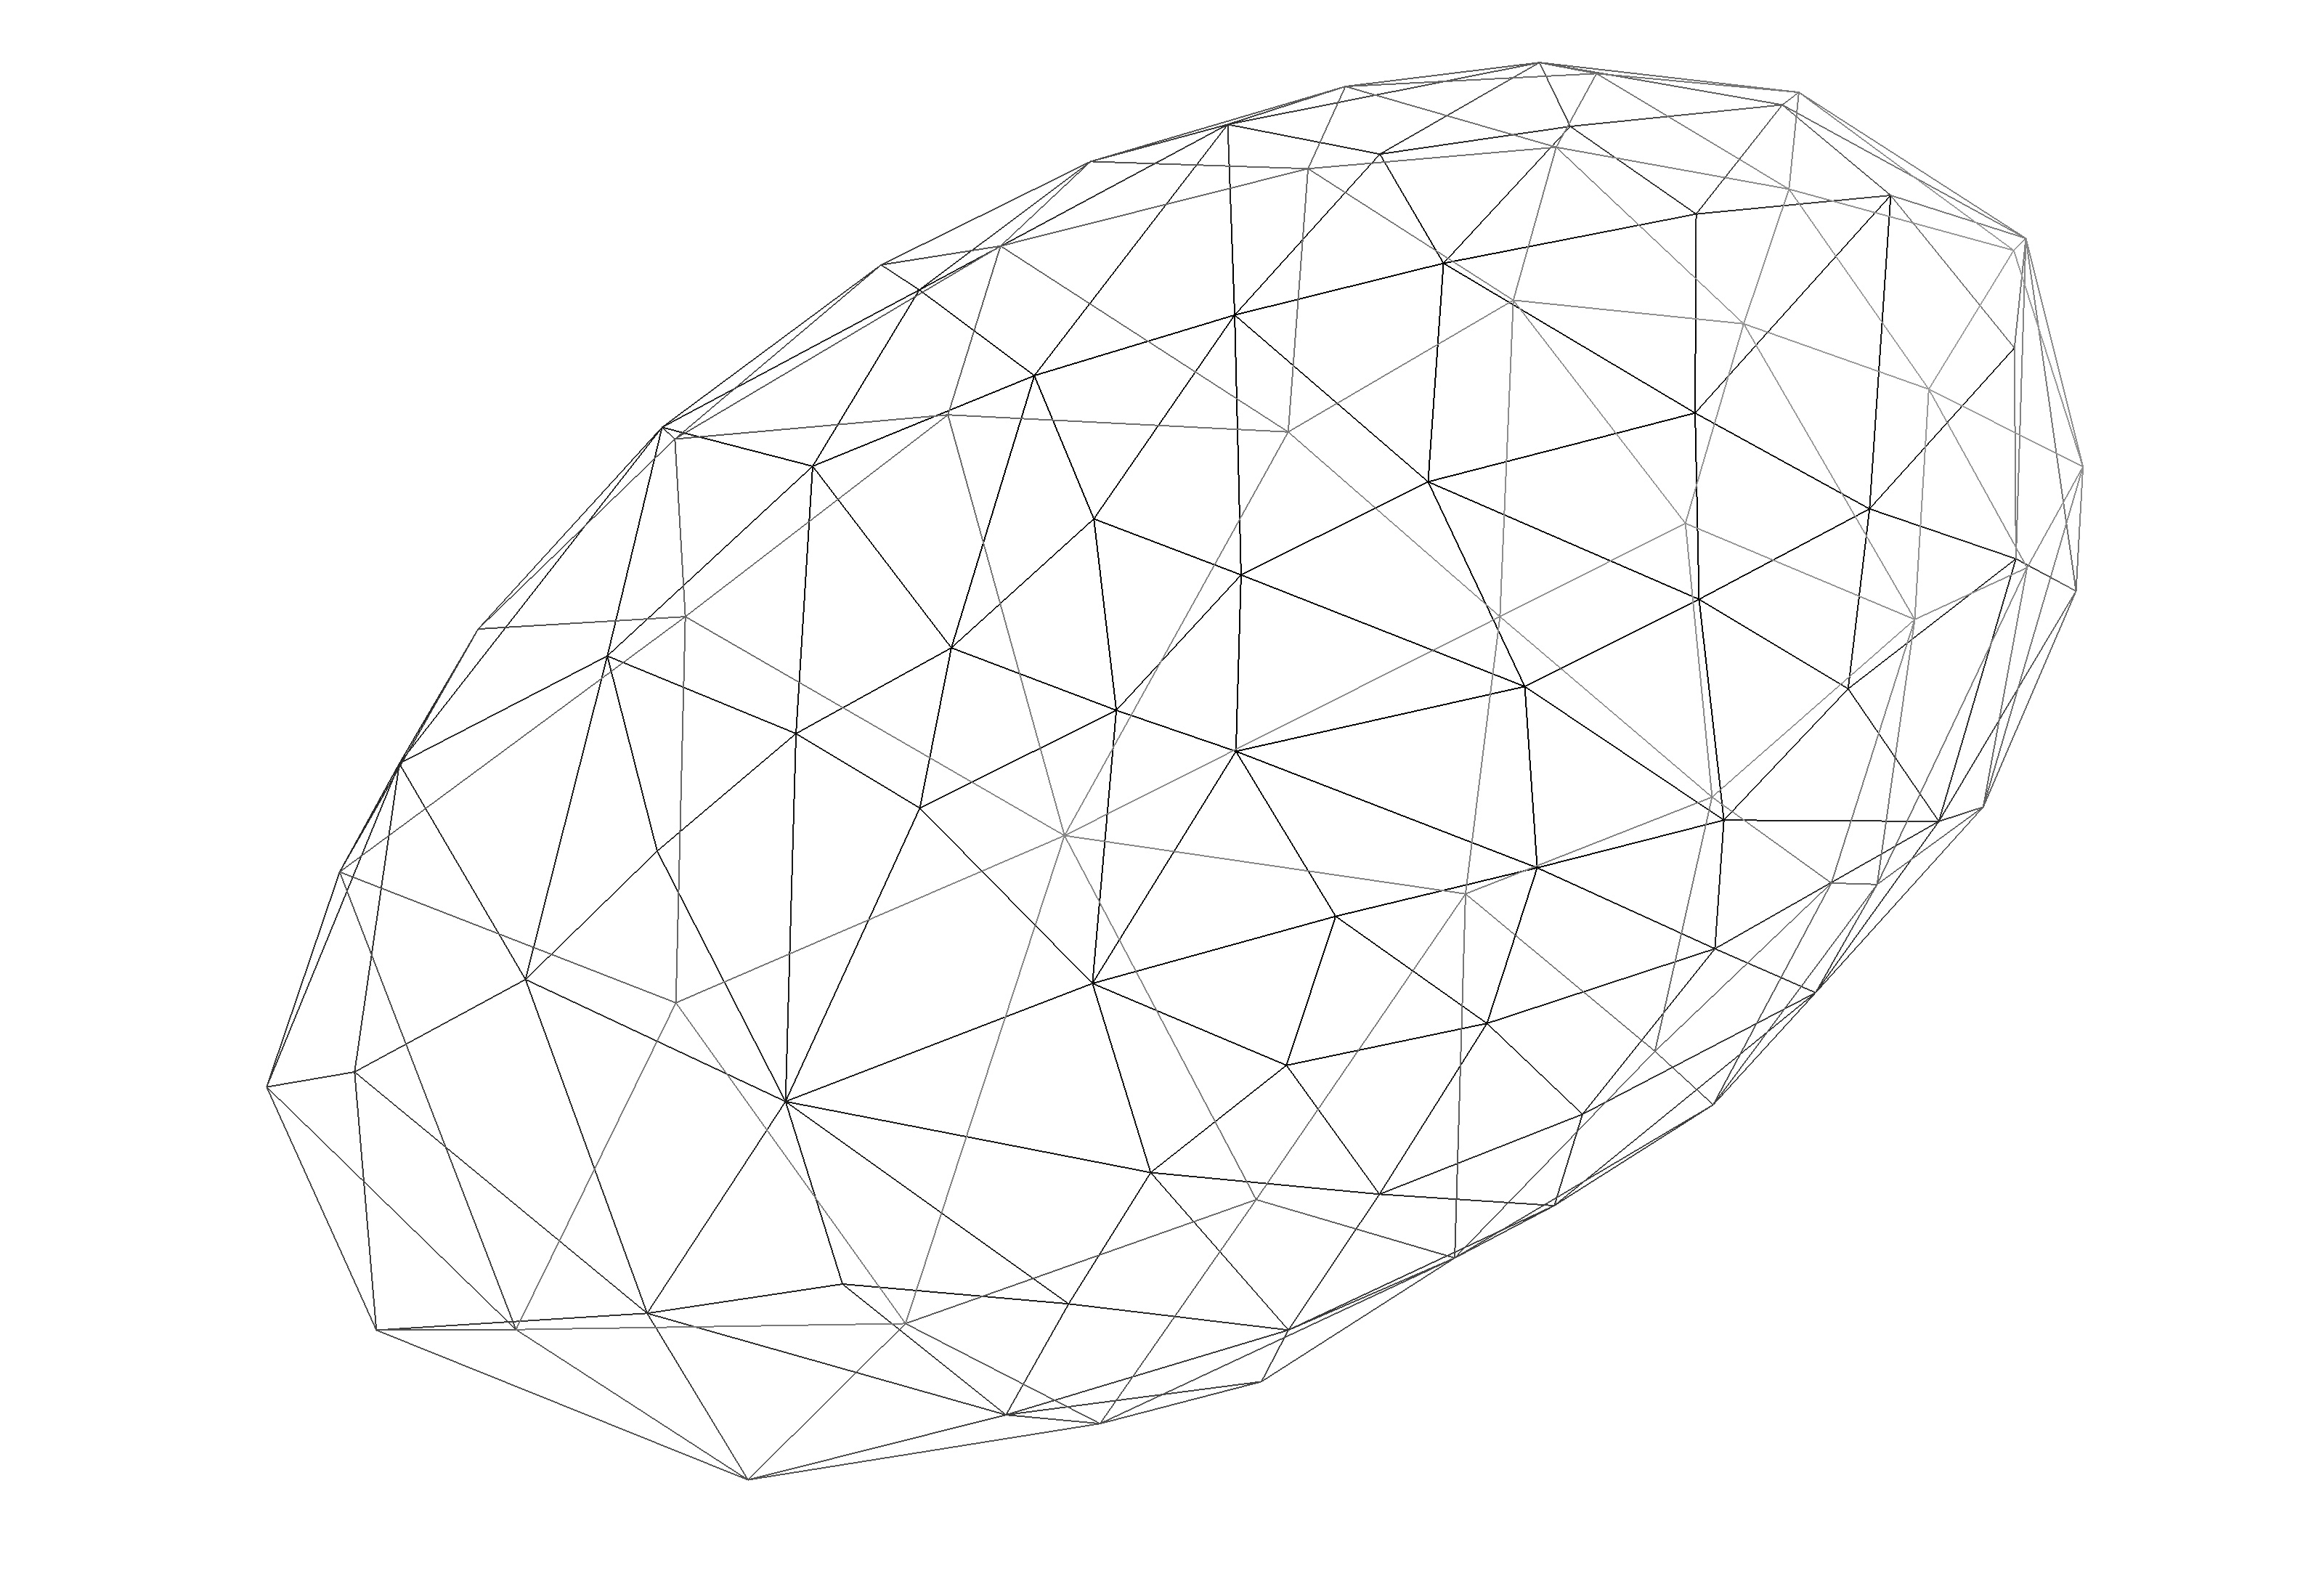
\includegraphics[trim={10cm 0 10cm 0}, clip,width=0.49\textwidth,keepaspectratio]{figures/computational_geometry/uniform_mesh_coarse.jpg}}
    \subcaptionbox{Fine Uniform Mesh\label{fig:fine_uniform_mesh}}{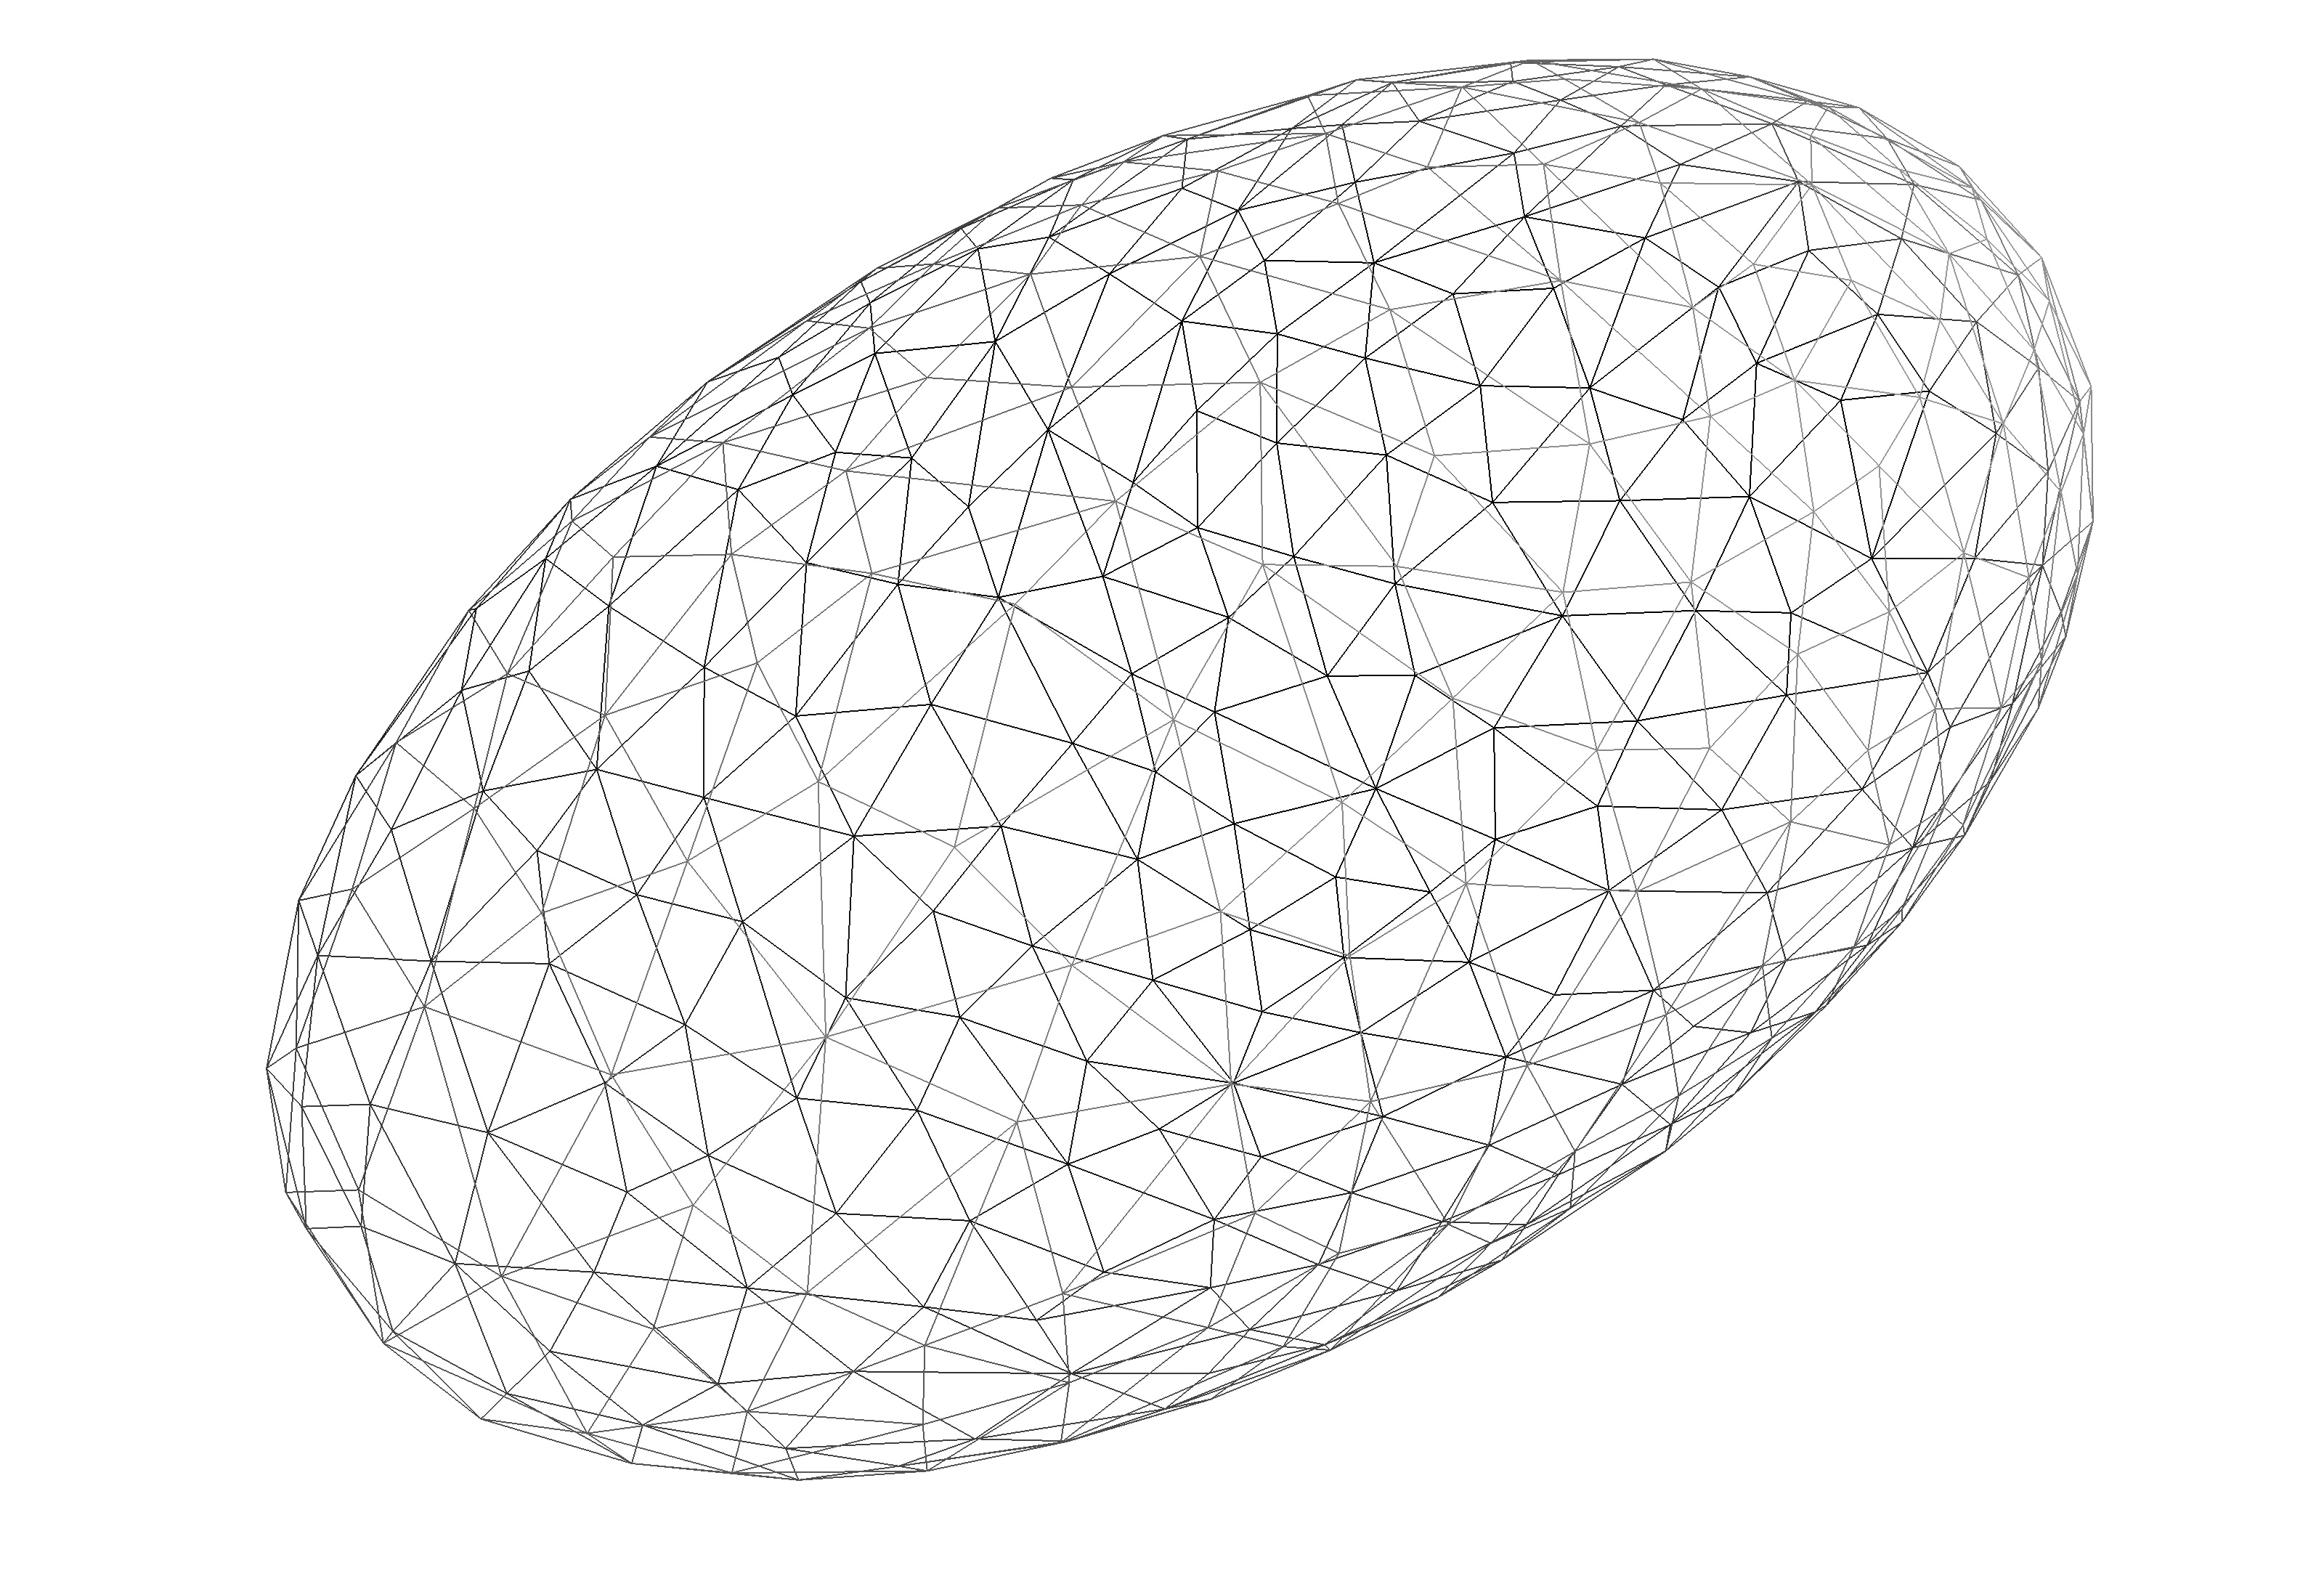
\includegraphics[trim={10cm 0 10cm 0}, clip,width=0.49\textwidth,keepaspectratio]{figures/computational_geometry/uniform_mesh_fine.jpg}}
    \caption{Examples of Resolution of Uniform Meshes of Triaxial Ellipsoid~\label{fig:uniform_mesh}}
\end{figure}

One of the first tasks for any spacecraft mission to a small body is to generate an estimate of the shape.
This shape model is used for a variety of purposes, such as the polyhedron potential model, like that presented in~\cref{sec:polyhedron_potential} or landing site section and guidance.
We assume that upon arrival at a target body, the spacecraft contains an initial estimate for the shape of the small body.
This shape can be a coarse estimate computed from ground measurements or it can be a triaxial ellipsoid based on the semimajor axes of the asteroid, such as that shown in~\cref{fig:uniform_mesh} which represents the maximum axes for asteroid Castalia.
Additionally, we assume that the shape estimate is closed and a triangular faceted surface mesh, emulating those used in practice to represent asteroids.
Furthermore, the number of vertices in the estimate can be scaled according to the desired final accuracy or computational capabilities.
For example,~\cref{fig:uniform_mesh} demonstrates two surface mesh representation for a triaxial ellipsoid at varying levels of detail. 
A wide variety of algorithms are available to generate a near uniformly spaced mesh for an arbitrary surface~\cite{persson2004,boissonnat2005}.

We assume the spacecraft contains a range sensor, such as \gls{lidar}, that allows for the accurate measurement of the relative distance between the spacecraft and asteroid~\cite{zuber1997,zuber2000}.
This type of sensor measures the round-trip time for a pulse of energy to leave the spacecraft, reflect off the surface, and return to a collector on board.
Given the time total time of flight, the distance can be accurately computed using \( d = \frac{\Delta TOF}{2 c} \) where \gls{sym:c} is the constant speed of light.
Assuming accurate knowledge of the pointing direction of the spacecraft, in the form of the rotation matrix \gls{sym:iatt}, we can compute a direction from the spacecraft to the measurement location on the surface.
The output of this sensor is a vector, \( \vc{d}_i \), defined in the spacecraft fixed frame which gives the direction to a measurement point on the surface. 
Using the state of the asteroid, we can transform this measurement to the asteroid fixed frame using the simple transformation
\begin{align*}
    \vc{p}_i = R_A^T R \vc{d}_i .
\end{align*}
Given many measurements, \( \vc{p}_i \in \R^3 \), of the asteroid surface we can efficiently update our initial shape estimate to that of the true surface.
\Cref{fig:lidar_example} shows asteroid 4769 Castalia and a representation of several LIDAR measurements. 
The spacecraft measures the range between itself and the asteroid surface to several points within the field of view of the sensor. 
These measurements provide a collection of points which lie on the surface of the asteroid, and by combining many points, a so called ``point cloud'', allows us to reconstruct the shape.
\begin{figure}
    \centering
    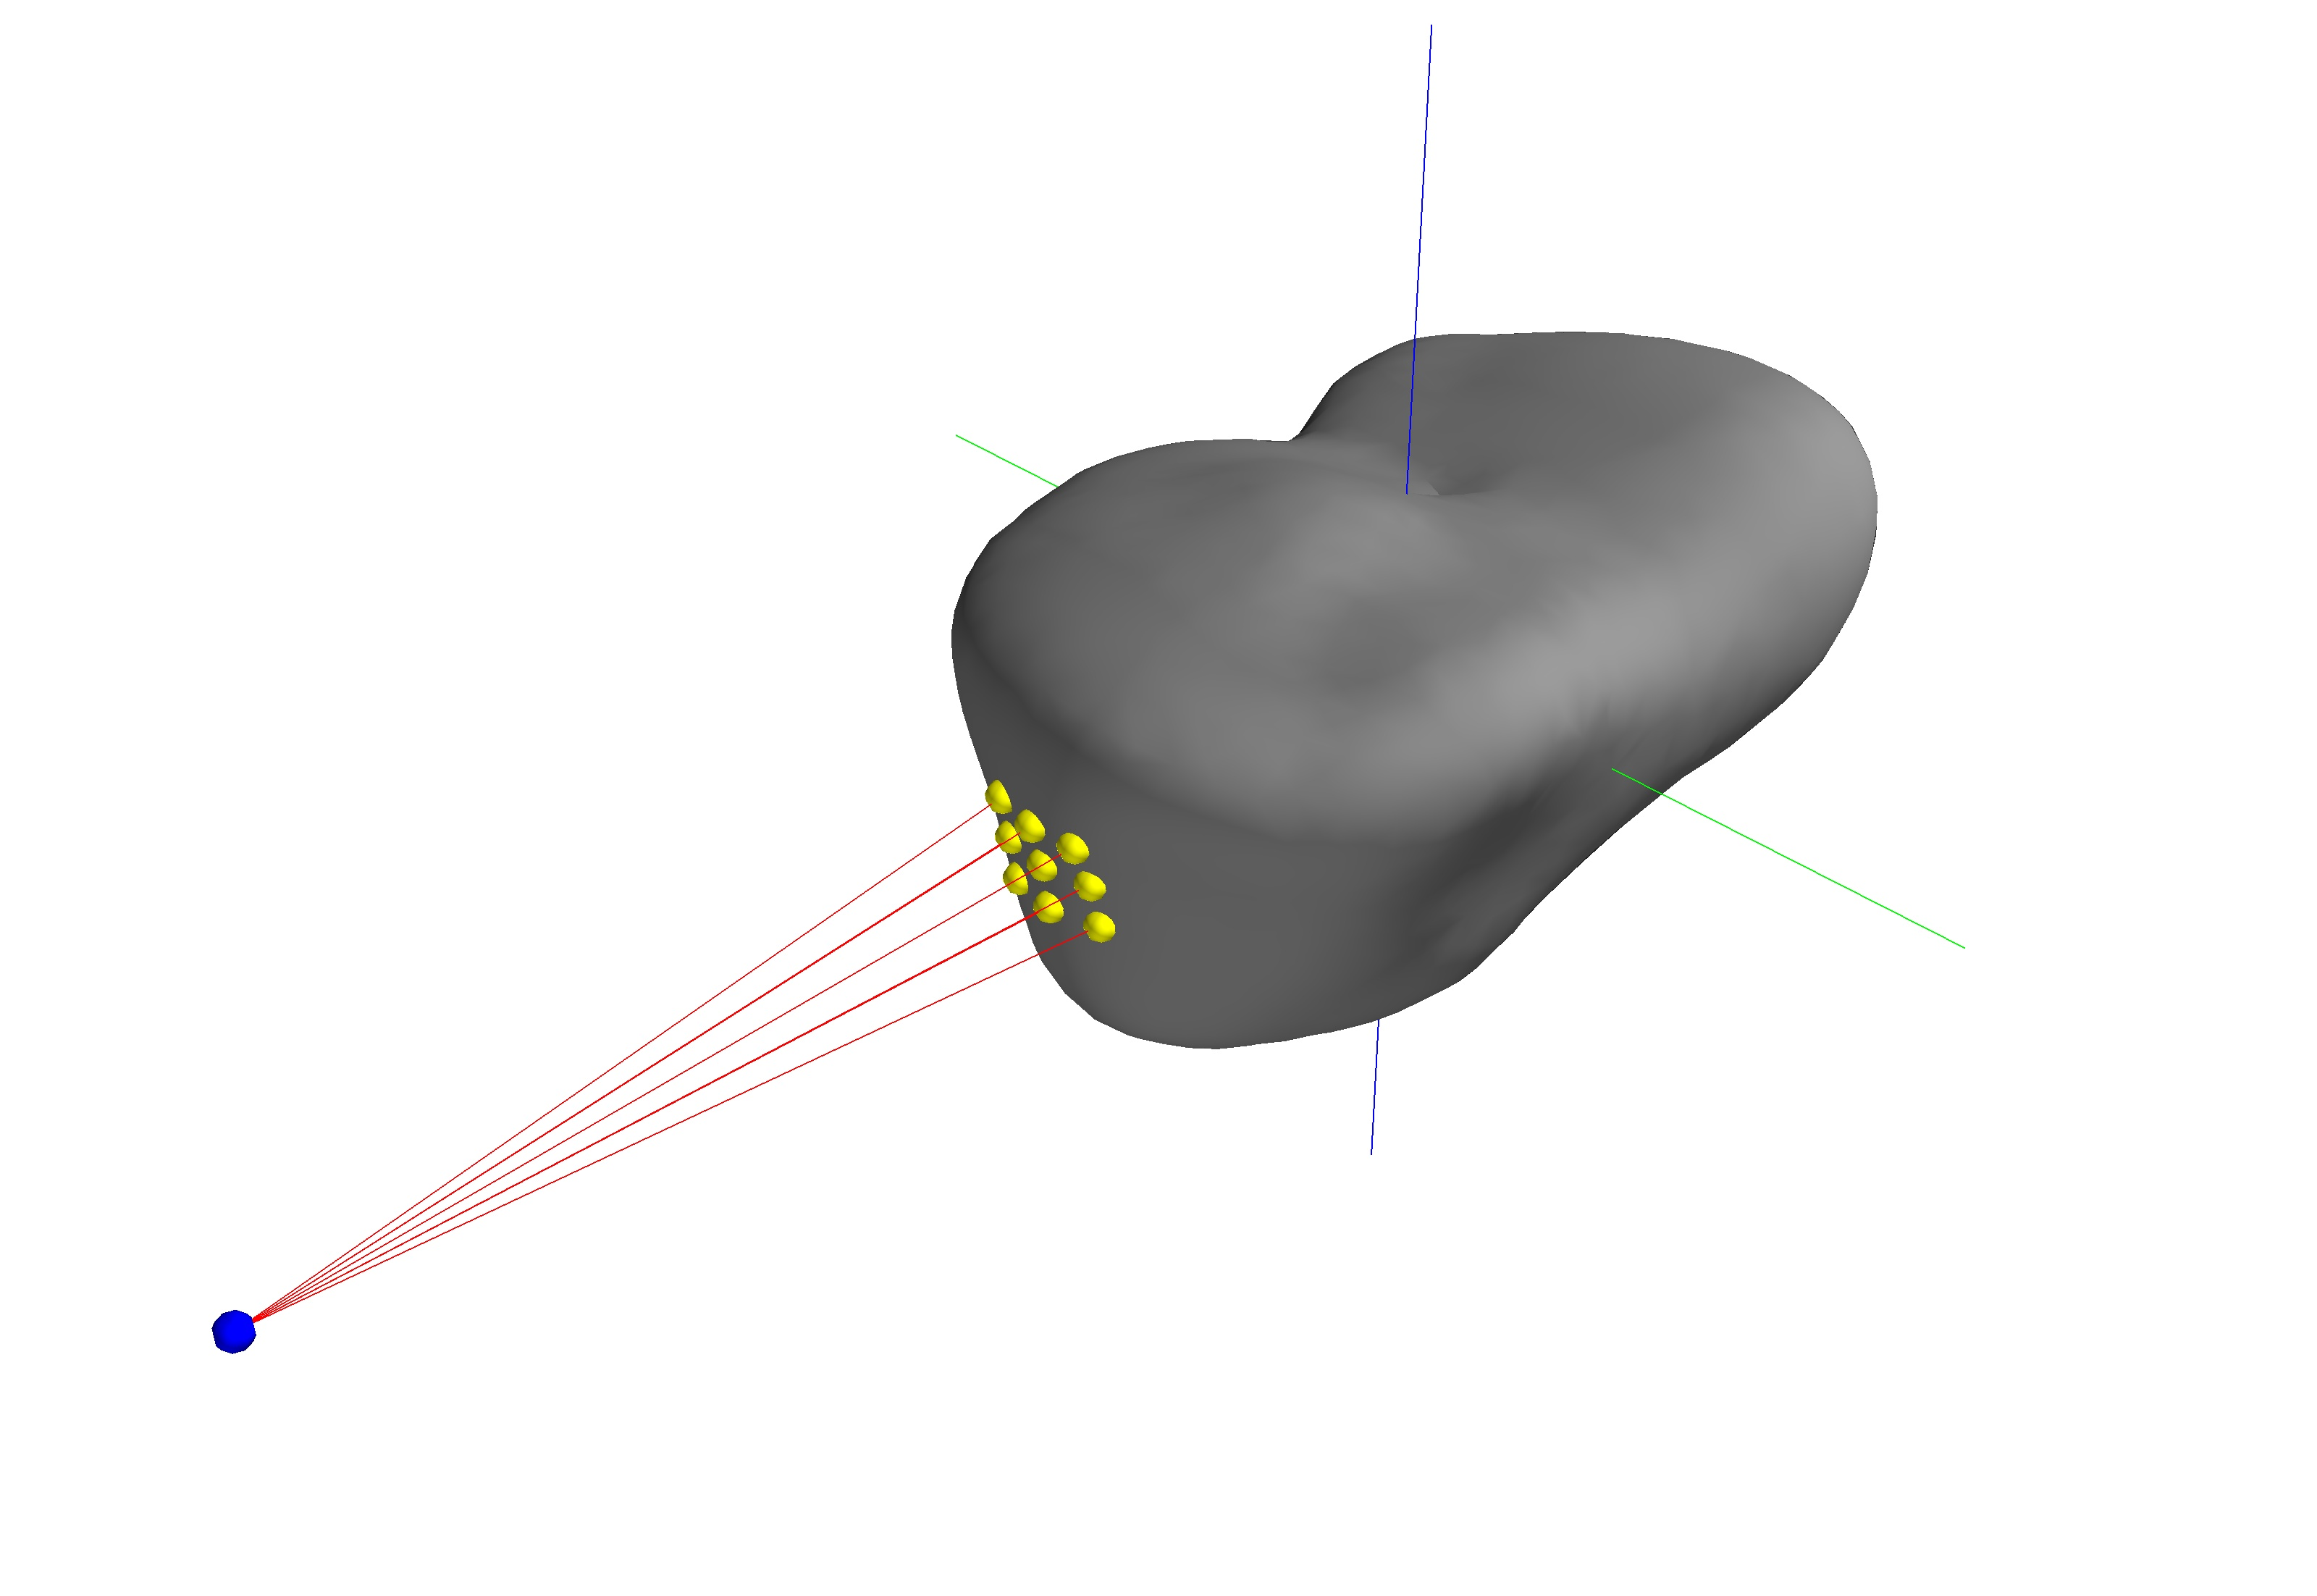
\includegraphics[width=0.75\textwidth]{figures/2018_SSPI/castalia_raycasting_plot.jpg}
    \caption{Simulated LIDAR measurements of asteroid Castalia~\label{fig:lidar_example}}
\end{figure}

\paragraph{Bayesian Shape Update}

Our algorithm applies a Bayesian framework to radially modify each vertex \( \vc{v}_i \in \R^3\) of the shape estimate based on measurement \( \vc{p}_i \in \R^3 \). 
This approach alleviates much of complexity of incorporating new vertices or surface triangulation common in surface reconstruction methods~\cite{berg2008}.
This assumption means that the total number of vertices of the shape model is fixed.
However, additional detail, in the form of additional vertices, is possible by using standard mesh subdivision algorithms~\cite{orourke1998}, which we later demonstrate in~\cref{sec:landing_refinement}.

The radial distance of each vertex, \( v_i = \norm{\vc{v}_i}\), is assumed to be distributed according to the Gaussian distribution
\begin{align*}
    v_i \sim \mathcal{N}(r_i, w_i^2)
\end{align*}
where \( r_i \) is the initial estimate of the radial distance of vertex \( \vc{v}_i\) and \( w_i \) is the initial variance, or confidence, in the radial distance.
The radial distance of each measurement, \( p_{j,i} = \norm{\vc{p}_j}\), is also assumed to be distributed according to the Gaussian distribution
\begin{align*}
    p_{j,i} \sim \mathcal{N}(r_{j,i}, w_{j,i}^2)
\end{align*}
where \( r_{j,i} = \norm{\vc{p}_{j,i}} \) defines the radial distance of the surface vector measurement and \( w_{j, i}\) defines the variance of the measurement with respect to vertex \( \vc{v}_i\).
Each measurement is defined by the index \( j \) while the associated vertex is defined by \( i \). 
As a result, the measurement \( p_{j, i} \) defines the distribution of measurement \( j \) with respect to vertex \( i \). 
Any given measurement may be used to update one or several vertices.

The variance for each measurement vector is assumed to be related to the ``distance'' from the measurement to vertex \( \vc{v}_i \).
Here, we use the \gls{geodesic} distance to parameterize the difference, and hence  uncertainty, of associating the measurement with a given vertex.
From spherical trigonometry~\cite{gade2010}, the central angle between measurement \( \vc{p}_i \) and vertex \( \vc{v}_i \) of the shape estimate is
\begin{align}\label{eq:geodesic_distance}
    \Delta \sigma_{j,i} = \arctan \parenth{\frac{\norm{\vc{p}_j \times \vc{v}_i}}{\vc{p}_j \cdot \vc{v}_i }}.
\end{align}
The variance of measurement \( \vc{p}_i \) with respect to vertex \( \vc{v}_i \) is then defined by the geodesic distance as
\begin{align}
    w_{j, i} = \norm{\vc{p}_j} \Delta \sigma_{j,i} .
\end{align}
This approach relates the uncertainty of the measurement \( \vc{p}_j \) with the geodesic distance to a given vertex, \( \vc{v}_i \).
As a result, measurements which are far from a vertex, i.e.\ \( \Delta \sigma \) is large, will tend to have a larger variance and hence uncertainty. 
This approach can be considered as a form of a correlation based sensor model~\cite{thrun2005}.
The main benefit of a correlation based approach, in contrast to feature extraction is the relative simplicity of implementation.
However, the resulting correlation values do not posses any physical significance and do not represent the noise or uncertainty characteristics of the sensor.

From Bayes' theorem, the posterior probability is defined as
\begin{align}
    p(v_i | p_{j, i}) = \frac{p(p_{j, i} | v_i) p(v_i)}{p( p_{j, i})} \propto p(p_{j,i} | v_i) p(v_i).
\end{align}
From the properties of a Gaussian, the posterior probability given a measurement is also distributed according to a Gaussian distribution~\cite{bishop2006} and given by
\begin{align}\label{eq:posterior_probability}
    \mathcal{N} \parenth{\frac{w_{j, i}^2 r_i + w_i^2 r_{j, i}}{w_i^2 + w_{j, i}^2} , \frac{w_i^2  w_{j, i}^2}{w_i^2 +  w_{j, i}^2}} .
\end{align}
From~\cref{eq:posterior_probability}, the posterior probability conditioned on the measurement is the weighted average of the prior knowledge and the measurement. 
Measurements that are far from the vertex will have a high uncertainty or variance and will have a reduced impact on the radial position of the vertex.
Additional measurements are incorporated using a weighted average of prior belief and the measurement uncertainty.

In order to improve the computational efficiency measurement updates are assumed to be local in nature.
Instead of applying a measurement to all vertices of the mesh, the measurement is only applied to the vertices which are within a specified region of the measurement. 
We define a region of interest, \( \Delta S \), about each measurement which defines the surface area over which the measurement will affect the mesh estimate.
We relate \( \Delta S \) to an equivalent angular constraint using
\begin{align}\label{eq:region_of_interest}
    \Delta \sigma_{max} = \sqrt \frac{\Delta S}{r_b^2}
\end{align}
% shankar: brillouin is correct. https://arc.aiaa.org/doi/10.2514/6.2014-4302
where \( r_b \) defines the Brillouin  sphere radius, or the radius of the circumscribing sphere of the asteroid.
Only vertices which satisfy \( \Delta \sigma_i \leq \Delta \sigma_{max} \) are considered in the Bayesian update shown in~\cref{eq:posterior_probability}.

The approach presented in this section allows one to update the shape of small body given a single range measurement of the surface.
A sequential process can be used to iteratively update the shape estimate given many measurements of the surface. 
For example,~\cref{sec:reconstruction_examples} shows the Bayesian update approach applied to several different asteroids.

\section{Optimal Guidance for Shape Reconstruction}\label{sec:explore_asteroid}

The mesh update algorithm presented in~\cref{sec:radius_update} does not offer a method to determine which portion of the surface needs to be updated. 
In this section, we present an optimal approach for the guidance of the vehicle in order to update the shape estimate.
Utilizing the nonlinear controllers developed in~\cref{sec:se3_control}, allows the spacecraft to maneuver to the best location that will update the shape estimate.
This guidance schemes enables autonomous operations around a small body.
% TODO talk about the basics of guidance/control for systems here and add tikz of block diagram

% \gls{gnc} refers to the design of systems to control the operations of vehicles, specifically automobiles, aircraft, or spacecraft.
% For spacecraft, many of these operations are computed ahead of time by operators and executed on board in an open loop fashion.
% Guidance refers to the determination of the desired future states, or trajectory, that the spacecraft should follow to achieve some goals.
% Navigation, or estimation, refers to the determination of the current state of the spacecraft given measurements.
% Control refers to the application of forces, \( u_m, u_f \), required by the spacecraft to follow the desired trajectory while maintaining stability and other criteria. 
% A block diagram representation of the entire \gls{gnc} system is shown in~\cref{fig:gnc}.
% The approach presented in this section addresses the guidance and control portions of \cref{fig:gnc} but does not address the navigation. 
% We assume that we have precise knowledge of the spacecraft state and small body rotation.

% \begin{figure}[htbp]
%     \centering
%     \includegraphics[width=\textwidth]{example-image-golden}
%     \caption{Block diagram of GNC system\label{fig:gnc}}
% \end{figure}

The ideal guidance approach involves solving a global optimal control problem which satisfies the system dynamics from~\cref{sec:dumbbell_model} while minimizing the shape uncertainty.
There are a wide variety of optimal control techniques which may be utilized to solve the problem, such as indirect methods based on the calculus of variations or direction methods based on solving a related nonlinear programming problem~\cite{kirk2012,bryson1975}.
The difficulty lies in implementing an algorithm that can operate in real time.
Since the \gls{lidar} will be operating at upwards of \SI{1}{\hertz} efficient processing of the measurement and computation of the guidance commands is critical.
Our approach solves this complexity by determining the vertex that should be measured to optimally update the shape estimate.

We define a cost associated with each vertex \( \vc{v}_i \) of the shape estimate
\begin{align}\label{eq:explore_cost}
    J_i (\ipos, \iatt, \aatt) = \alpha_w J_{w_i} + \alpha_d J_{d_i}(\rpos) + \alpha_c J_{c_i}(\rpos)
\end{align}
where the weighting factors \( \alpha_w, \alpha_d, \alpha_c \in \R^1 \) are chosen such that \( \alpha_w + \alpha_d + \alpha_c = 1 \).
The cost function is defined as a function of the current inertial position, \gls{sym:ipos}, and the attitude, \gls{sym:iatt} of the spacecraft.
Furthermore, knowledge of the small body rotation is required in order to determine the position of the spacecraft in the small body fixed frame, \( \gls{sym:rpos} = \gls{sym:aatt}[^T] \gls{sym:ipos}\).

The term \( J_{w_i} \in \R^1 \) represents the cost associated with the uncertainty of vertex \( i \) as
\begin{align}\label{eq:weight_cost}
    J_{w_i} &= - \frac{w_i}{w_m}
\end{align}
where \( w_i \) is the uncertainty of vertex \( i \) and \( w_m \) is a maximum uncertainty used to scale the values.
The term \( J_{d_i} \) represents the scaled geodesic distance between the current state of the spacecraft and vertex \( i \),
\begin{align}\label{eq:distance_cost}
    J_{d_i}(\rpos) &= \frac{1}{\pi} \arctan \parenth{ \frac{\norm{\rpos \times \vc{v}_i}}{\rpos \cdot \vc{v}_i}}.
\end{align}

Finally, a control component is included in the cost function which penalizes vertices that are difficult to reach.
Consider, the current position of the spacecraft in the small body fixed frame as \( \rpos\) and a desired vertex \( \vc{v}_i \) of the shape estimate.
We can define a normal vector to the plane spanned by \( \rpos, \vc{v}_i \) as
\begin{align}\label{eq:normal_to_plane}
    \vc{n}_i = \frac{\rpos \times \vc{v}_i}{\norm{\rpos} \norm{\vc{v}_i}}.
\end{align}
Then a trajectory \( x_d(\theta) \) as
\begin{align}\label{eq:spherical_waypoint}
    x_d(\theta) = r_d \exp{\parenth{\theta \hat{\vc{n}_i}} } \frac{\rpos}{\norm{\rpos}},
\end{align}
where \( \theta : \bracket{0, \frac{\rpos \cdot \vc{v}_i}{\norm{\rpos}\norm{\vc{v}_i}}} \to \R^1\) parameterizes the desired trajectory.
\Cref{eq:spherical_waypoint} simply describes a portion of a great circle trajectory between the current state, \( \rpos \), and the desired vertex \( \vc{v}_i \)~\cite{chen2016}.
The altitude of the spacecraft, \( r_d \in \R \), can be chosen based on sensor characteristics of safety concerns.
For example, \( r_d \) can be chosen as the distance of the Biroullin sphere with an additional safety margin to mitigate any surface collision~\cite{scheeres2012a}.
The translational controller presented in~\cref{eq:translational_control} is used to determine the control input to follow \( x_d\).
We assume that the tracking errors are small, such that \( e_x, e_v \) are negligible, therefore the control becomes
\begin{align}\label{eq:tracking_control_cost}
    u_f(\theta) = -F_{ext}(x_d(\theta)), 
\end{align}
where the external force is defined by the polyhedron potential model given in~\cref{eq:inertial_velocity_dynamics}.
The control cost is then defined as the integral over the desired trajectory~\cref{eq:spherical_waypoint} between the current state and the desired vertex as
\begin{align}\label{eq:control_cost}
    J_{c_i}(\rpos) = \frac{1}{u_m} \int_{\theta_0}^{\theta_f} u_f(\theta)^T R u_f(\theta) d\theta,
\end{align}
where \( u_m \) is used to normalize and scale \( J_{c_i} \).
\Cref{eq:control_cost} is numerically integrated over the trajectory \( x_d(t) \) and used to penalize vertices which have a larger cost.

The vertex which minimizes~\cref{eq:explore_cost} 
\begin{align*}
    \vc{v}_{min} = \min_{i} J_i(\ipos, \iatt, \aatt),
\end{align*}
is determined and used to determine the optimum vertex of the shape model to measure.
This vertex is then used to determine the required state of the spacecraft in order to collect a measurement.
We assume that the spacecraft will maneuver to a location directly above the selected vertex, \( \vc{v}_{min} \), and point in the nadir direction to collect a measurement.
The desired state is transformed into the inertial frame and chosen as a location above \( \vc{v}_{min} \) as
\begin{align}
    \ipos_d = r_d \aatt \vc{v}_{min}, 
\end{align}
where \( r_d \) is again chosen to ensure a safety margin above the surface.
The desired attitude command, \( R_d\), is chosen such that the spacecraft camera axis, \( \vc{b}_1 \), is directed along the nadir towards the small body.
It is sufficient to define two orthogonal vectors to uniquely determine the attitude of the spacecraft.
The \( \vc{b}_{3d} \) vector is chosen to lie in the plane spanned by \(\vc{b}_{1d} \) and \( \vc{e}_3 = \vc{f}_3 \).
The desired attitude command is defined as
\begin{align}
    \vc{b}_{1d} &= - \frac{\vc{x}}{\norm{\vc{x}}} , \\
    \vc{b}_{3d} &= \frac{\vc{f}_3 - \parenth{\vc{f}_3 \cdot \vc{b}_{1d}} \vc{b}_{1d}}{\norm{\vc{f}_3 - \parenth{\vc{f}_3 \cdot \vc{b}_{1d}} \vc{b}_{1d}}}, \\
    \vc{b}_{2d} &= \vc{b}_{3d} \times \vc{b}_{1d} , \\
    R_d &= \begin{bmatrix} \vc{b}_{1d} & \vc{b}_{2d} & \vc{b}_{3d} \end{bmatrix} .
\end{align}
This form of \( R_d \) will direct the \( \bvec{1} \) axis towards the small body, and can be modified for a different camera orientation.

\section{Multi-resolution Landing Area Refinement}\label{sec:landing_refinement}

The shape update approach presented in~\cref{sec:radius_update} is designed with autonomous operations in mind. 
It is based on an initial coarse shape estimate that is iteratively updated with range measurements of the surface.
Furthermore, the original mesh is uniformly distributed and as a result many small topological features such as rocks or small craters are not be captured by the shape model. 
However, these small features are critical for surface operations and safe landings.
In addition, it would be computationally prohibitive to have a uniformly high resolution mesh.
In this section, we extend the previous shape update approach to enable a much higher fidelity in a specific location.

Mixed resolution surface meshes are routinely used in finite element and geometric modeling applications~\cite{botsch2010}.
As shown in~\cite{mcmahon2017}, utilizing mixed resolution shape models for asteroid missions offers the potential of reduced computational demands.
The computational cost of the polyhedron potential model, given by~\cref{eq:potential}, is roughly proportional to the number of faces in the shape model.
As a result, a uniformly high resolution shape would quickly become intractable for real time operations.
However, utilizing a mixed resolution approach allows for a high fidelity in a smaller mission critical area, such as a landing site, with a limited impact on the computational cost.

The selection of a landing site will typically require a vast quantity of data and weigh a multitude of possible metrics, such as scientific value, hardware constraints, timing and communication limits, or safety considerations. 
In our analysis we consider the surface slope, the distance to the surface, and a fictitious science metric in order to determine the best landing site based on the complete shape estimate.
This approach allows for a spacecraft to autonomously select and land on small body.

The surface slope is computed according to the method developed in~\cite{scheeres1996}.
Due to the small size, and therefore low gravitational attraction, the force at each point on the surface is a combination of the gravitational attraction and the centripetal acceleration.
At the center of each face, \( f_i = \begin{bmatrix} f_x & f_y & f_z \end{bmatrix} \), we compute a modified surface acceleration as
\begin{align}\label{eq:surface_force}
    U_m = \omega^2 \begin{bmatrix} f_x \\ f_y \\ 0 \end{bmatrix} + \begin{bmatrix} U_x \\ U_y \\ U_z \end{bmatrix},
\end{align}
where \( \omega \in \R^1 \) is the angular velocity of the asteroid and \( U_i \) is computed from~\cref{eq:attraction}.
Then the surface slope can be computed from
\begin{align}\label{eq:surface_slope}
    \cos \parenth{ \pi - \phi } = \frac{\vc{n}_f \cdot U_m}{\norm{U_m}},
\end{align}
where \( \phi \in \R^1 \) is the surface slope defines the angle between the surface normal \( \vc{n}_f \in \R^3 \) and the force vector at the surface.
If \( \phi = \SI{0}{\degree} \) then the force vector and the surface normal are anti-parallel, while \( \phi > \SI{90}{\degree} \) means that a particle on the surface would be thrown off the body as the centripetal force is larger than the gravitational attraction.

Additionally, we compute the distance, using~\cref{eq:geodesic_distance}, between the spacecraft state and each face of the asteroid. 
Finally, we also assign a random science value to the surface in the form of two dimensional Gaussian.
Utilizing these metric, a landing site is chosen to minimize the surface cost given as
\begin{align}\label{eq:surface_cost}
    J_l =  J_{\text{distance}} - J_{\text{science}},
\end{align}
where the surface slope is considered a hard constraint such that any candidate landing site must satisfy \( \phi \leq \phi_m \).

\paragraph{Mesh Refinement}\label{sec:refinement}

Once a suitable landing site is selected, the surrounding area is isolated and refined by adding new vertices and faces in the specified area.
The goal of refinement, or more generally remeshing, is given a mesh ( or a portion of it), compute another mesh whose elements satisfy some quality metrics while suitably approximating the original mesh.
In this work, we utilize the isotropic remeshing algorithm implemented in \gls{cgal}.
This algorithm uses an iterative method which repeatedly splits long edges, collapses short edges, and relocates vertices until all edges are approximately the desired target edge length.
% TODO Think about adding PMP 6.12 image here

For example,~\cref{fig:cube_remesh} shows the isotropic remeshing result for the selected faces of a unit cube.
The original unit cube is composed of \num{8} vertices and \num{12} faces.
The two triangular faces of the visible side of the cube are selected for the isotropic remeshing operation as shown in~\cref{fig:cube_original_mesh}.
A target edge length of \num{0.1} is selected for these faces and used to generate~\cref{fig:cube_refine_mesh}.
The two large triangular faces are divided into a number of smaller triangular faces.
Furthermore, the additional faces are all approximately the same size and preserve the original surface of the cube.
After the isotropic remeshing operation the number of vertices has increased from \num{8} to \num{140}.
\begin{figure}[htbp]
    \centering
    \subcaptionbox{Original Cube\label{fig:cube_original_mesh}}{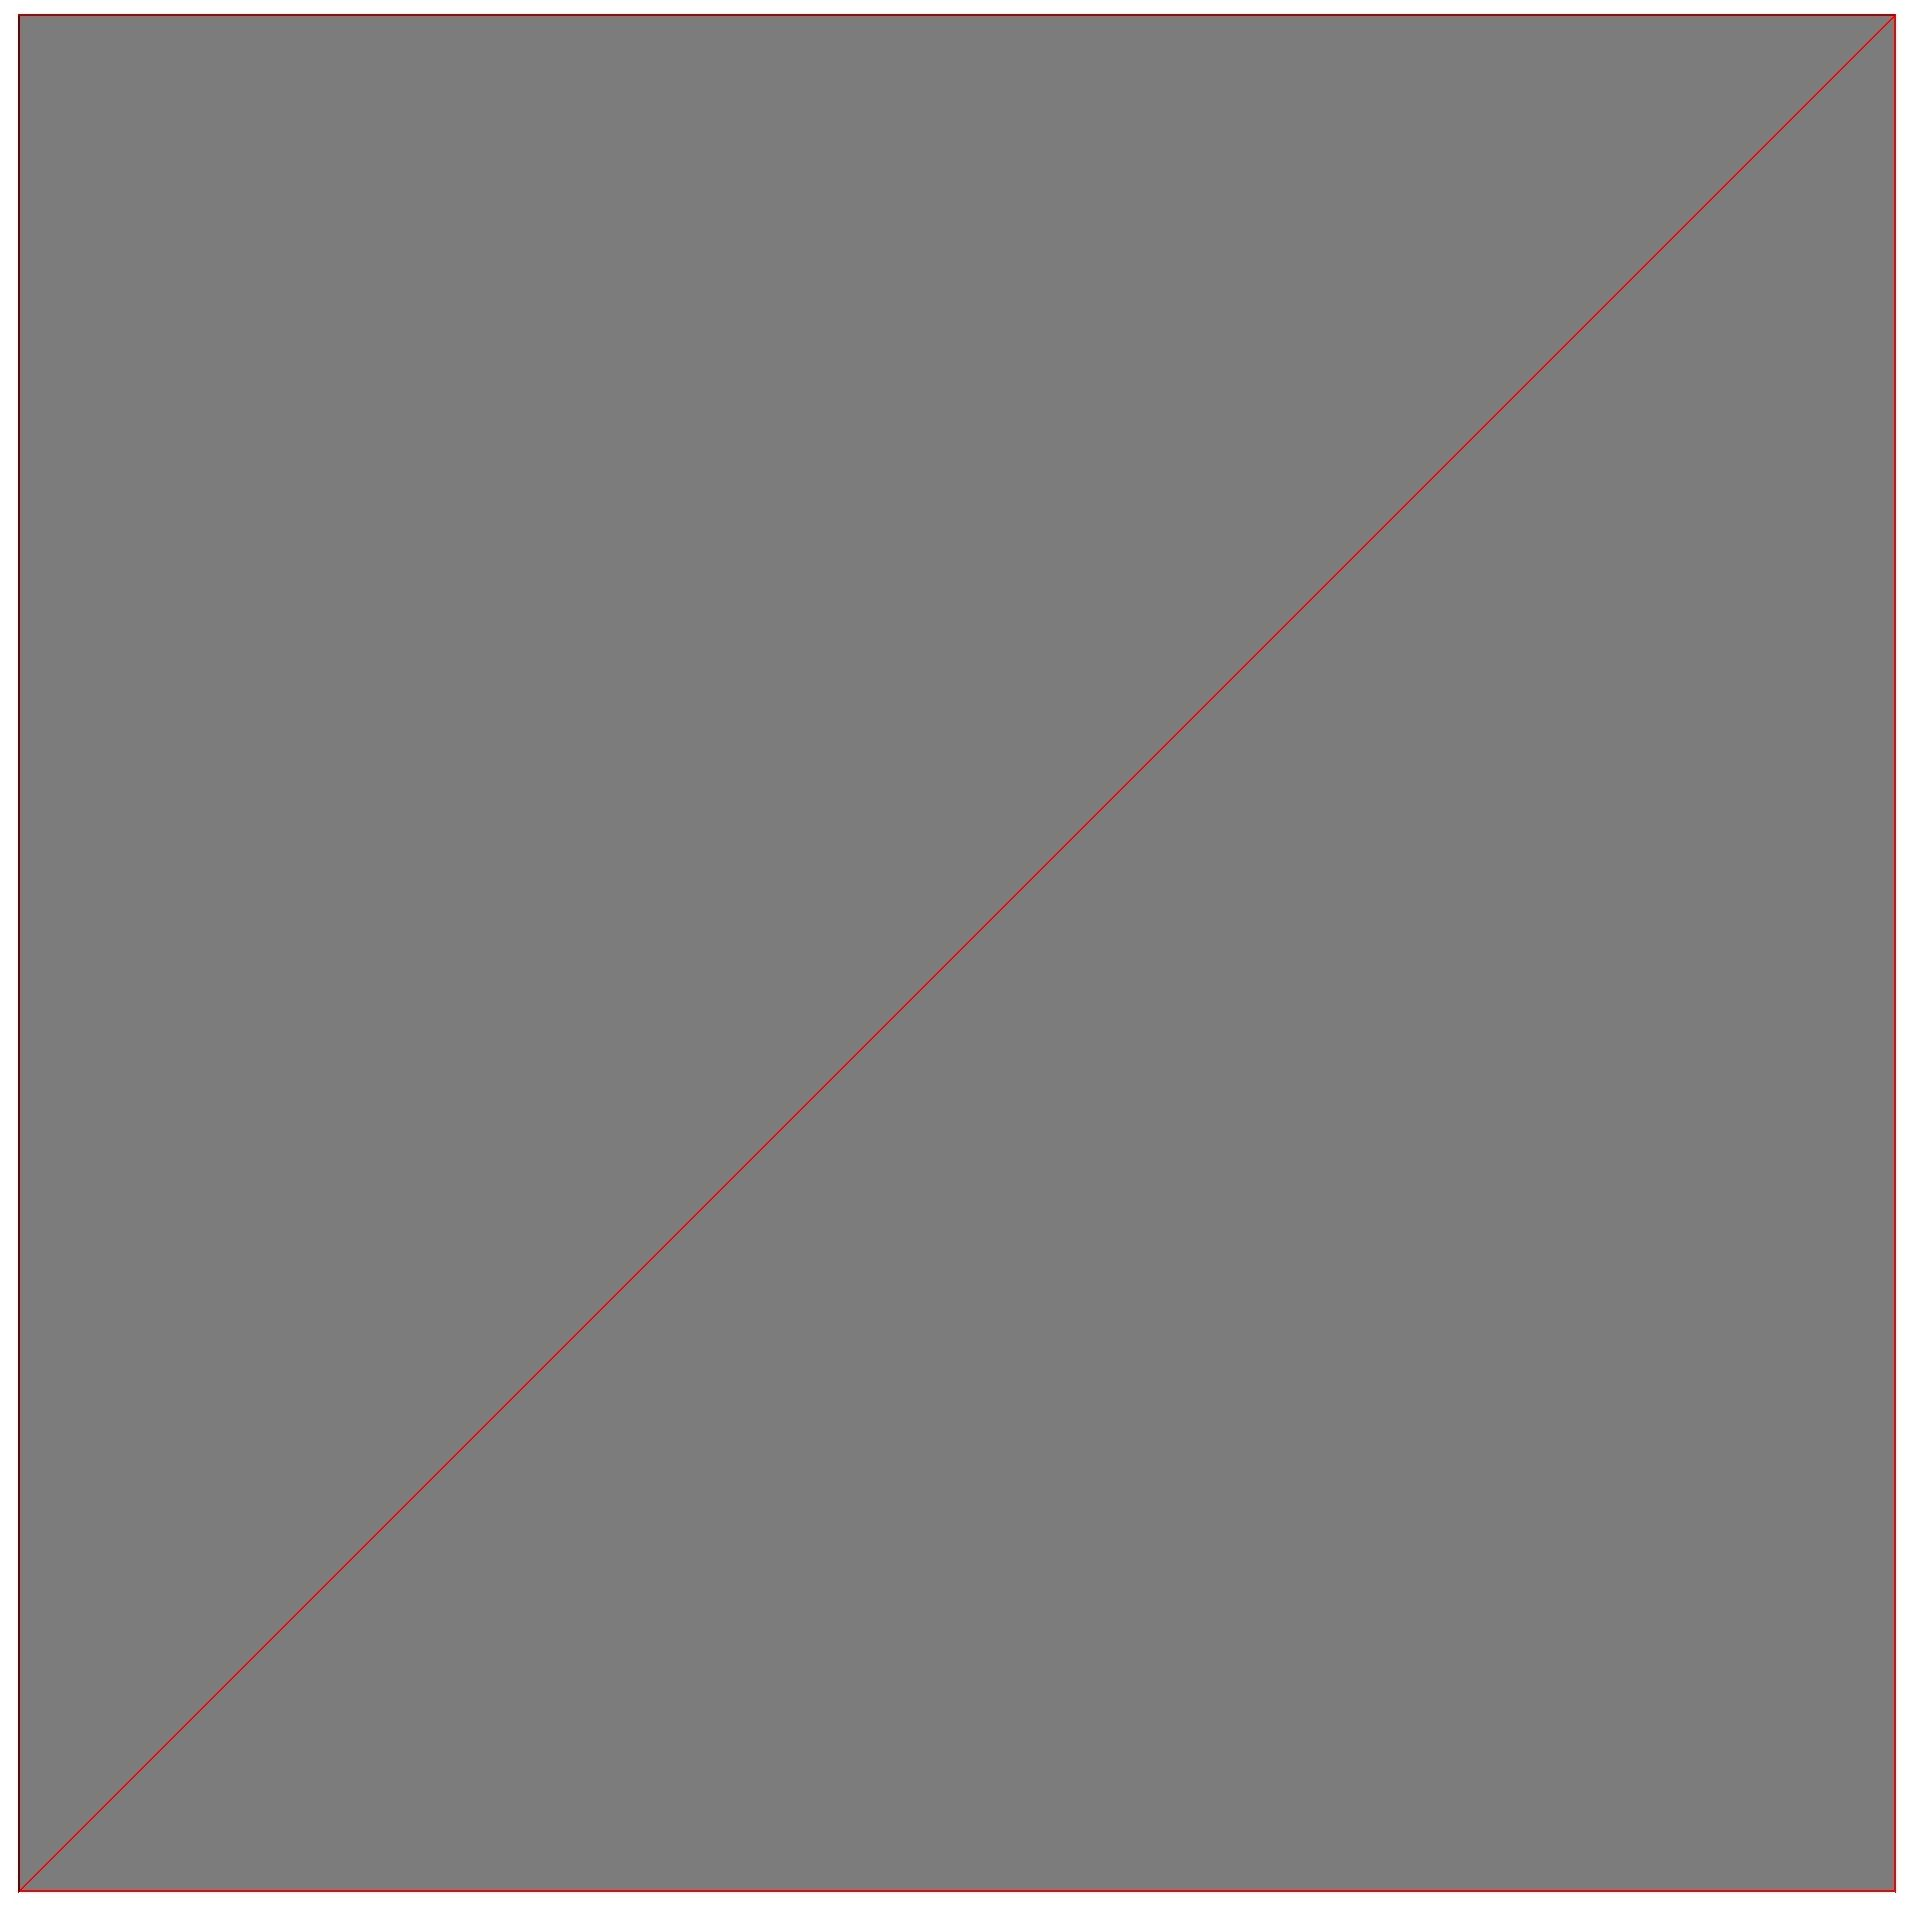
\includegraphics[width=0.49\textwidth]{figures/computational_geometry/isotropic/original_cube.jpg}}~
    \subcaptionbox{Remeshed Cube\label{fig:cube_refine_mesh}}{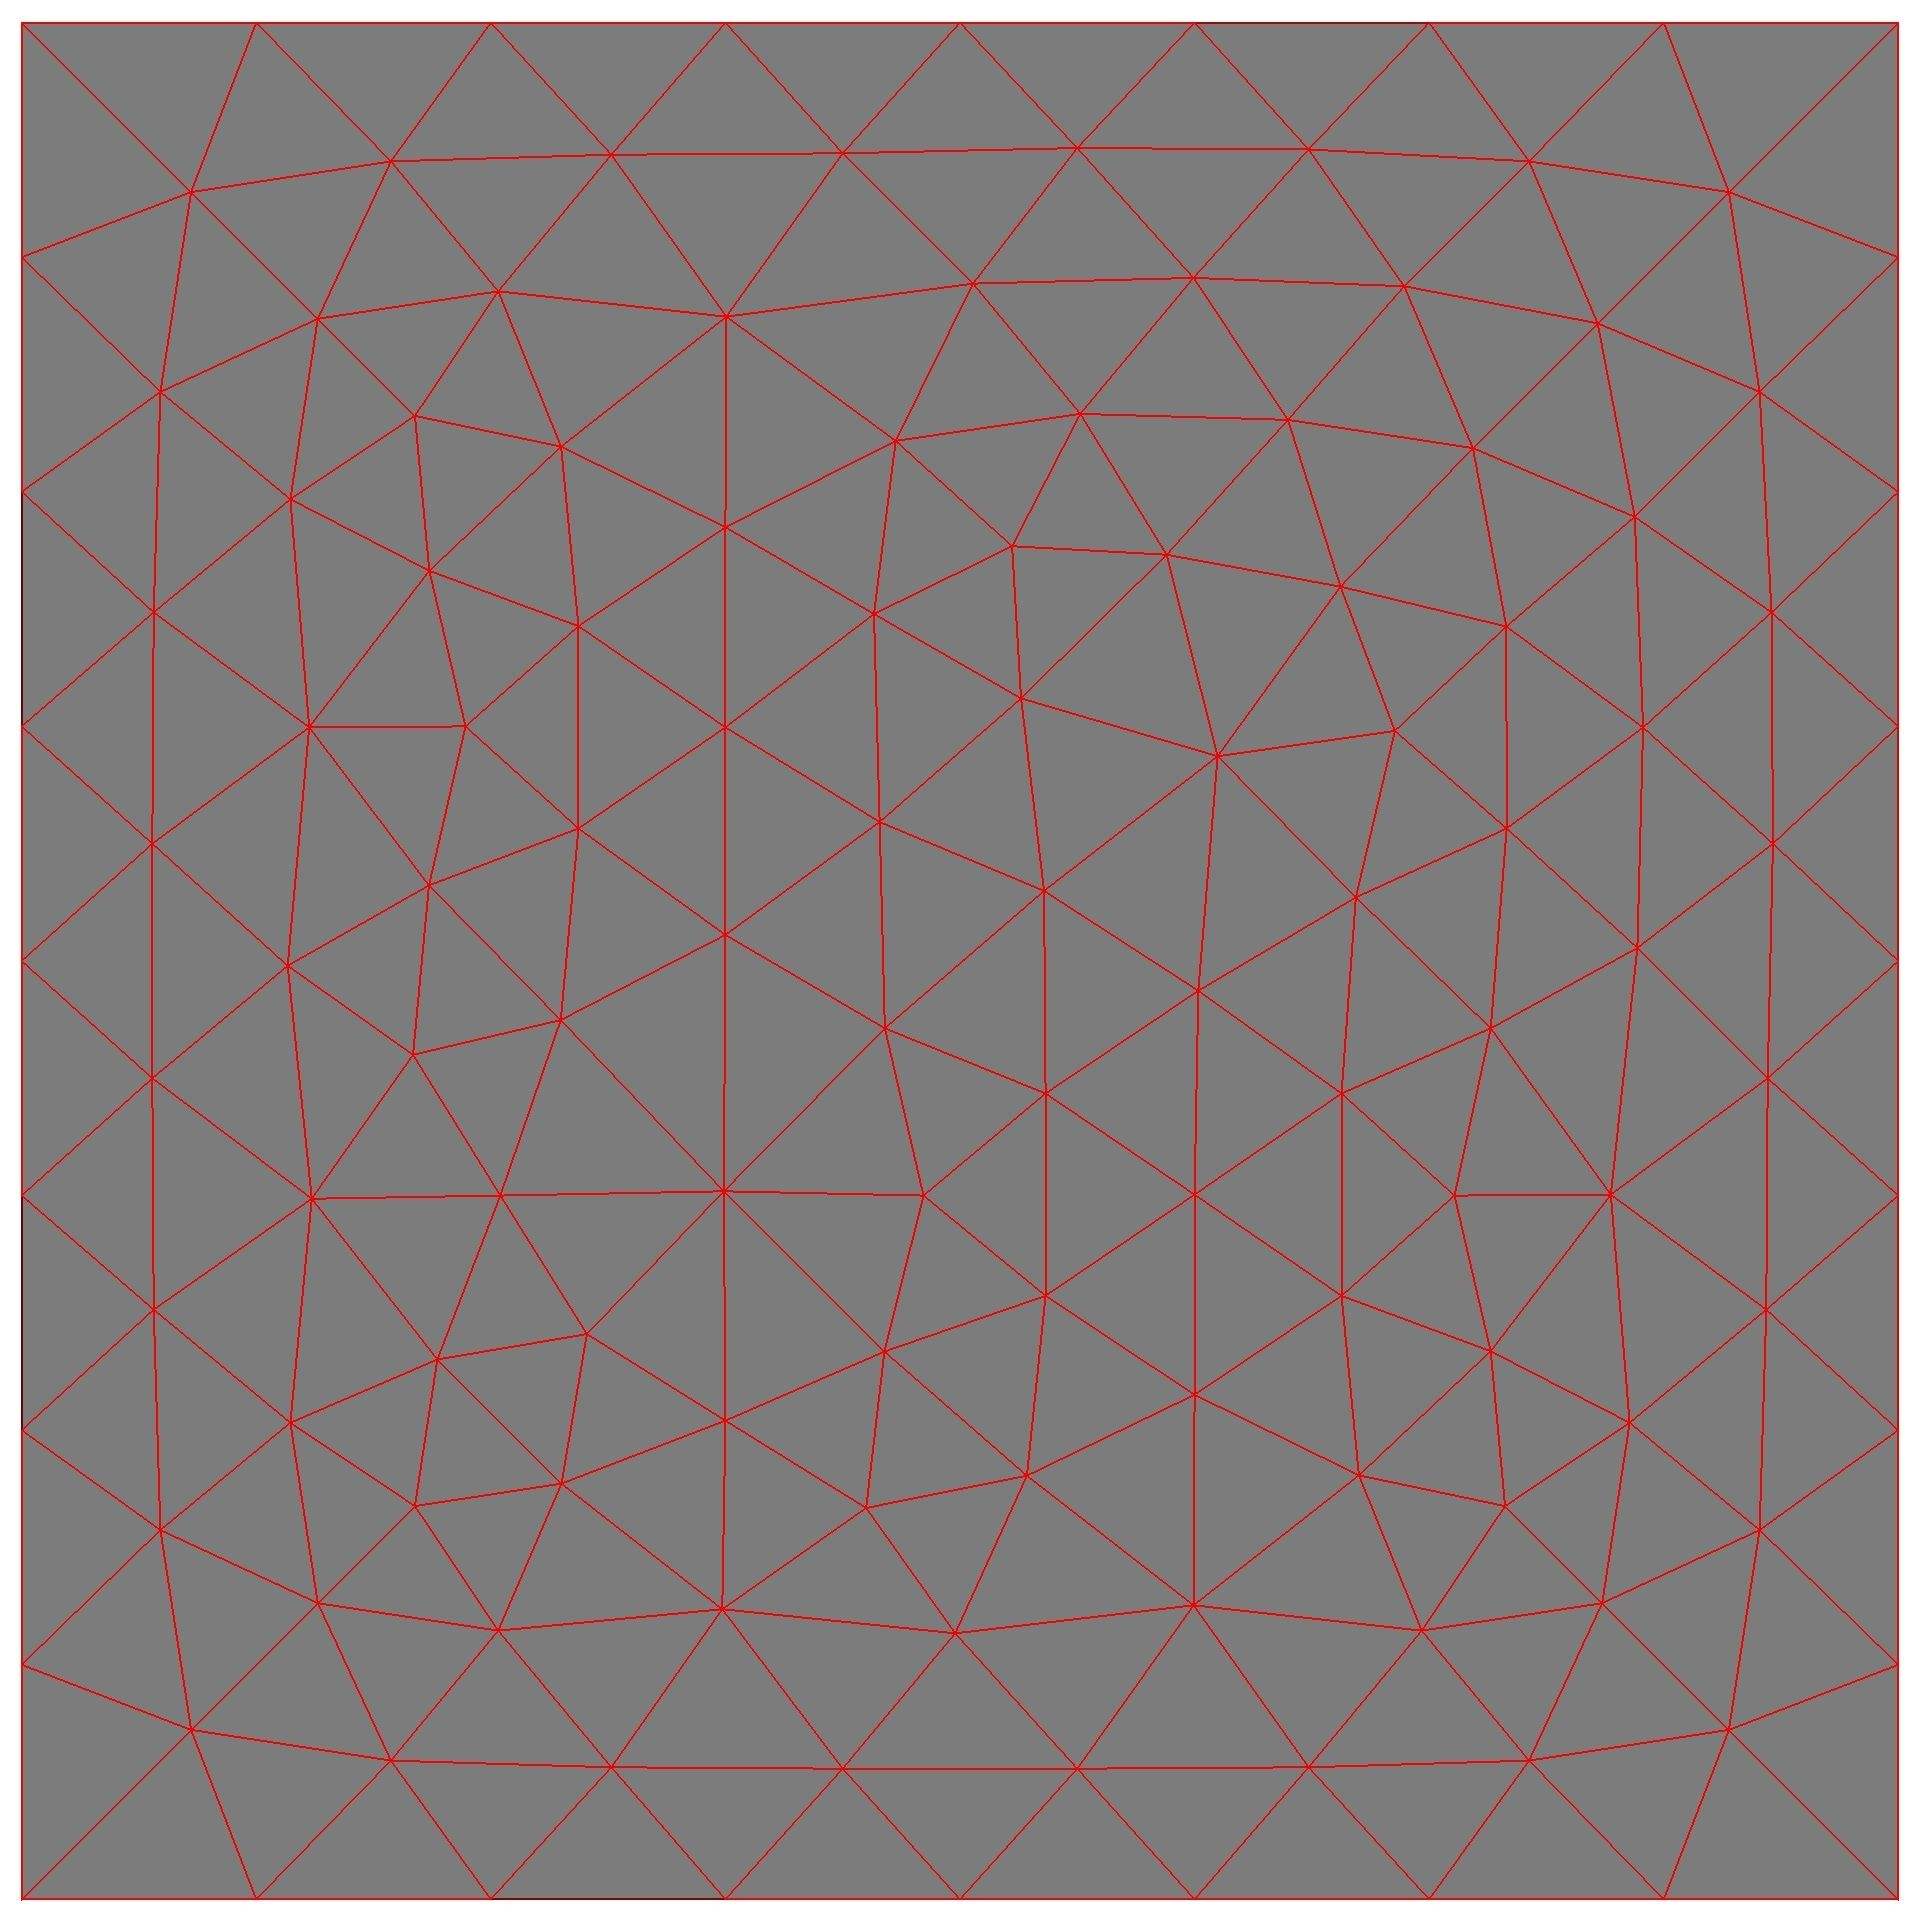
\includegraphics[width=0.49\textwidth]{figures/computational_geometry/isotropic/remesh_cube.jpg}}
    \caption{Example of isotropic remeshing of a face of a cube\label{fig:cube_remesh}}
\end{figure}

In order to demonstrate the multi resolution surface refinement we require a true shape model that contains small scale surface features.
In this dissertation, we utilize the true radar shape model of asteroid 4769 Castalia.
However, the shape model is not highly detailed as it does not contain small craters or surface features.
In order to apply the landing refinement process we augment a small portion of the mesh with some additional features and utilize the mesh update scheme in~\cref{sec:radius_update} to measure the surface.
The augmented model of Castalia is shown in~\cref{fig:castalia_refinement}.
\Cref{fig:castalia_refinement} shows that the increased resolution is required in order to reconstruct these small surface details.


\section{Numerical Examples}\label{sec:reconstruction_examples}

In this section, we demonstrate the use of the results presented in~\cref{sec:mathematical_background,sec:se3_control,sec:shape_reconstruction} with several numerical examples.
The incremental shape reconstruction approach from~\cref{sec:radius_update} is used to iteratively reconstruct the shape of several asteroid given \gls{lidar} measurements.
We utilize radar shape models of asteroids \num{4769} Castalia, (\num{52760}) \num{1998} \(\text{ML}_{14}\), \num{1620} Geographos, and 6489 Golevka~\cite{neese2004}.
The asteroids exhibit a wide range of shapes and demonstrate the effectiveness of the mesh update approach.
\Cref{sec:kinematic_exploration} focuses on the application of the incremental mesh update scheme of~\cref{sec:radius_update} for several different asteroids.
\Cref{sec:dynamic_exploration} incorporates the full dynamic model on \( \SE \) of a dumbbell spacecraft given in~\cref{sec:inertial_dumbbell_eoms}, the polyhedron potential model from~\cref{sec:polyhedron_potential}, and the mesh update and guidance scheme presented in~\cref{sec:radius_update}.

\subsection{Shape Reconstruction}\label{sec:kinematic_exploration}

The results in this section utilize a kinematics only model of the spacecraft and dynamics instead of the full dynamic simulation. 
We ignore the dynamics of the asteroid and spacecraft and instead focus solely on the shape reconstruction.
\Cref{tab:kinematic_asteroids} lists the true shape model parameters of asteroids Geographos and Golevka.
\begin{table}[htbp]
    \centering
    \begin{tabular}{lccc}
        \toprule
        Asteroid & Semi-major axes (\si{\kilo\meter}) & Vertices & Faces\\
        \midrule
        \num{1620} Geographos & \( 2.5 \times 1.0 \times 1.05 \) & \num{8192} & \num{16380}  \\
        \num{6489} Golevka & \( 0.53 \times 0.53 \times 0.53 \)  & \num{2048} & \num{4092} \\
        \bottomrule
    \end{tabular} 
    \caption{Asteroid properties for kinematic only exploration~\label{tab:kinematic_asteroids}}
\end{table}
The spacecraft is assumed to be able to arbitrarily move around the asteroid and collect measurements.
The simulations begin with an triaxial ellipsoid mesh that is sized to match the semi-major axes of each asteroid.
With this estimate, measurements are made of the surface and used to reconstruct the true shape following the process in~\cref{sec:radius_update}.
\Gls{lidar} measurements are generated until the total uncertainty
\begin{align*}
    \sum_i w_i,
\end{align*}
is sufficiently small.
In addition, we compute the volume of the estimate shape throughout the simulation using the algorithm presented in~\cref{sec:polyhedron_volume}.

\begin{figure}[htbp]
    \centering
    \subcaptionbox{Initial Shape Estimate\label{fig:geographos_partial_0}}{\includegraphics[trim={20cm 15cm 20cm 15cm}, clip,width=0.5\textwidth,keepaspectratio]{figures/computational_geometry/mesh_update/geographos/partial_0.jpg}}%
    \subcaptionbox{\SI{25}{\percent} of measurements added\label{fig:geographos_partial_25}}{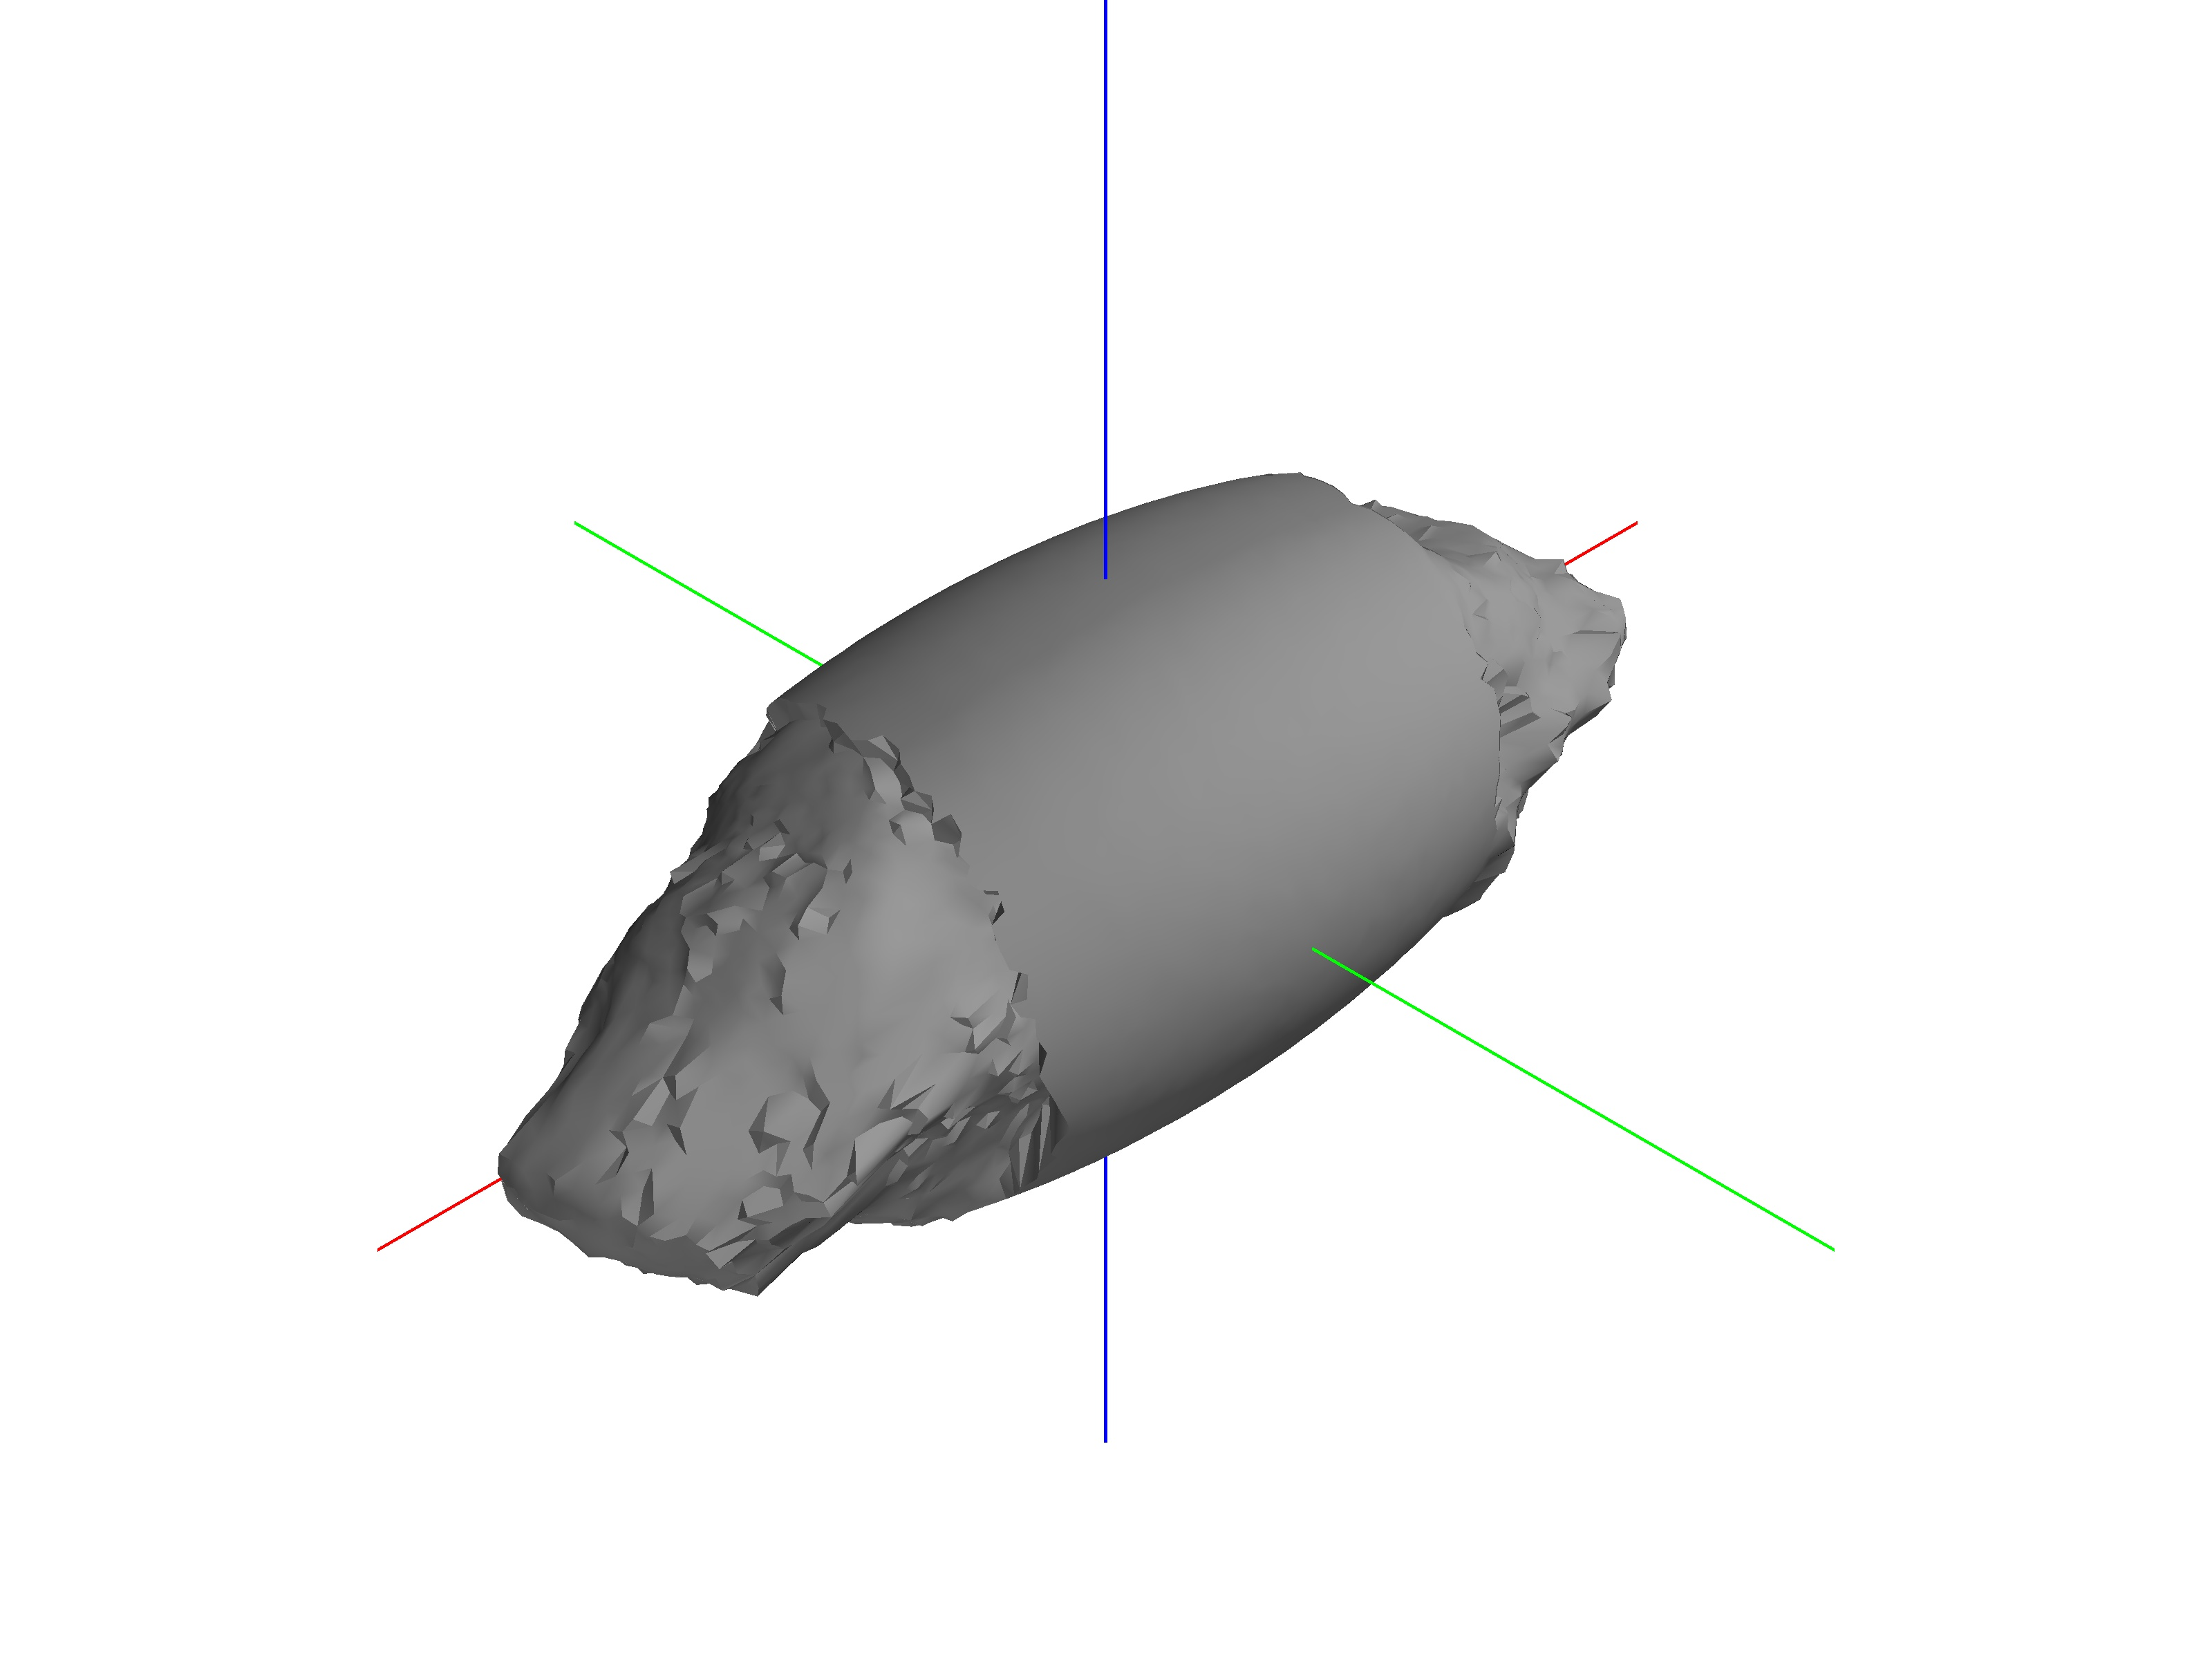
\includegraphics[trim={20cm 15cm 20cm 15cm},clip,keepaspectratio,width=0.5\textwidth]{figures/computational_geometry/mesh_update/geographos/partial_1872.jpg}}

    \subcaptionbox{\SI{50}{\percent} of measurements added\label{fig:geographos_partial_50}}{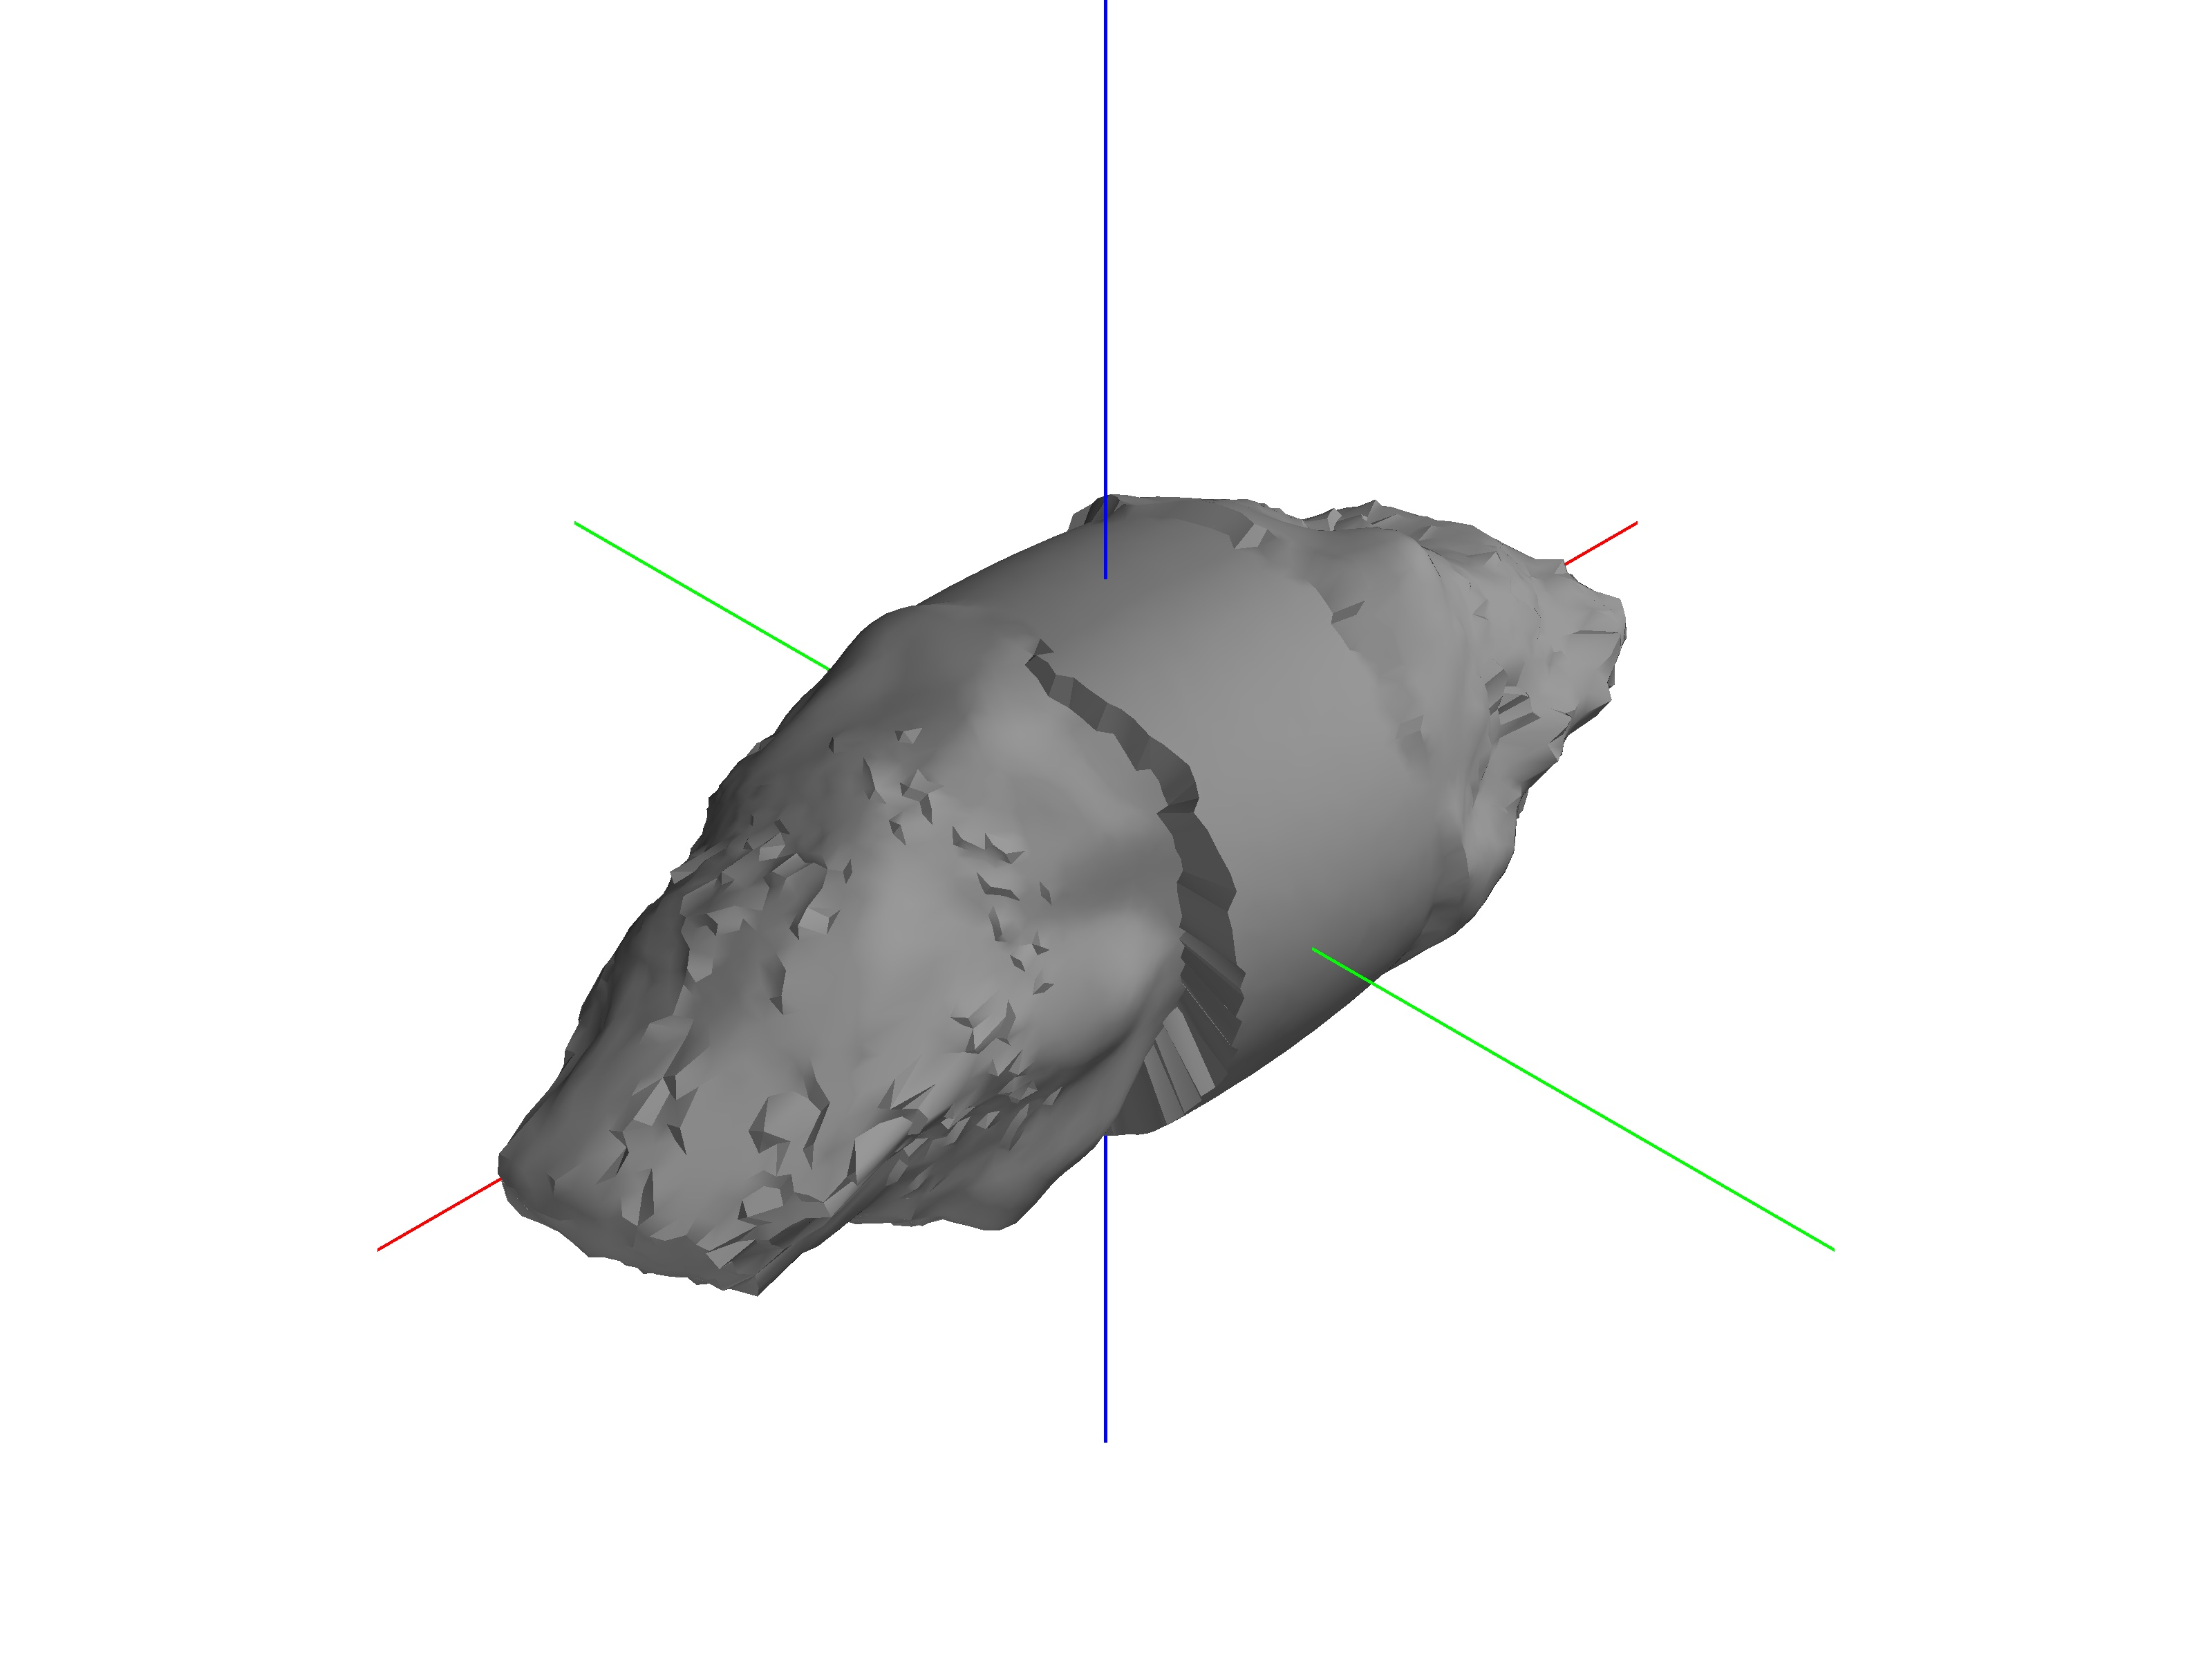
\includegraphics[trim={20cm 15cm 20cm 15cm},clip,keepaspectratio,width=0.5\textwidth]{figures/computational_geometry/mesh_update/geographos/partial_3745.jpg}}%
    \subcaptionbox{\SI{75}{\percent} of measurements added\label{fig:geographos_partial_75}}{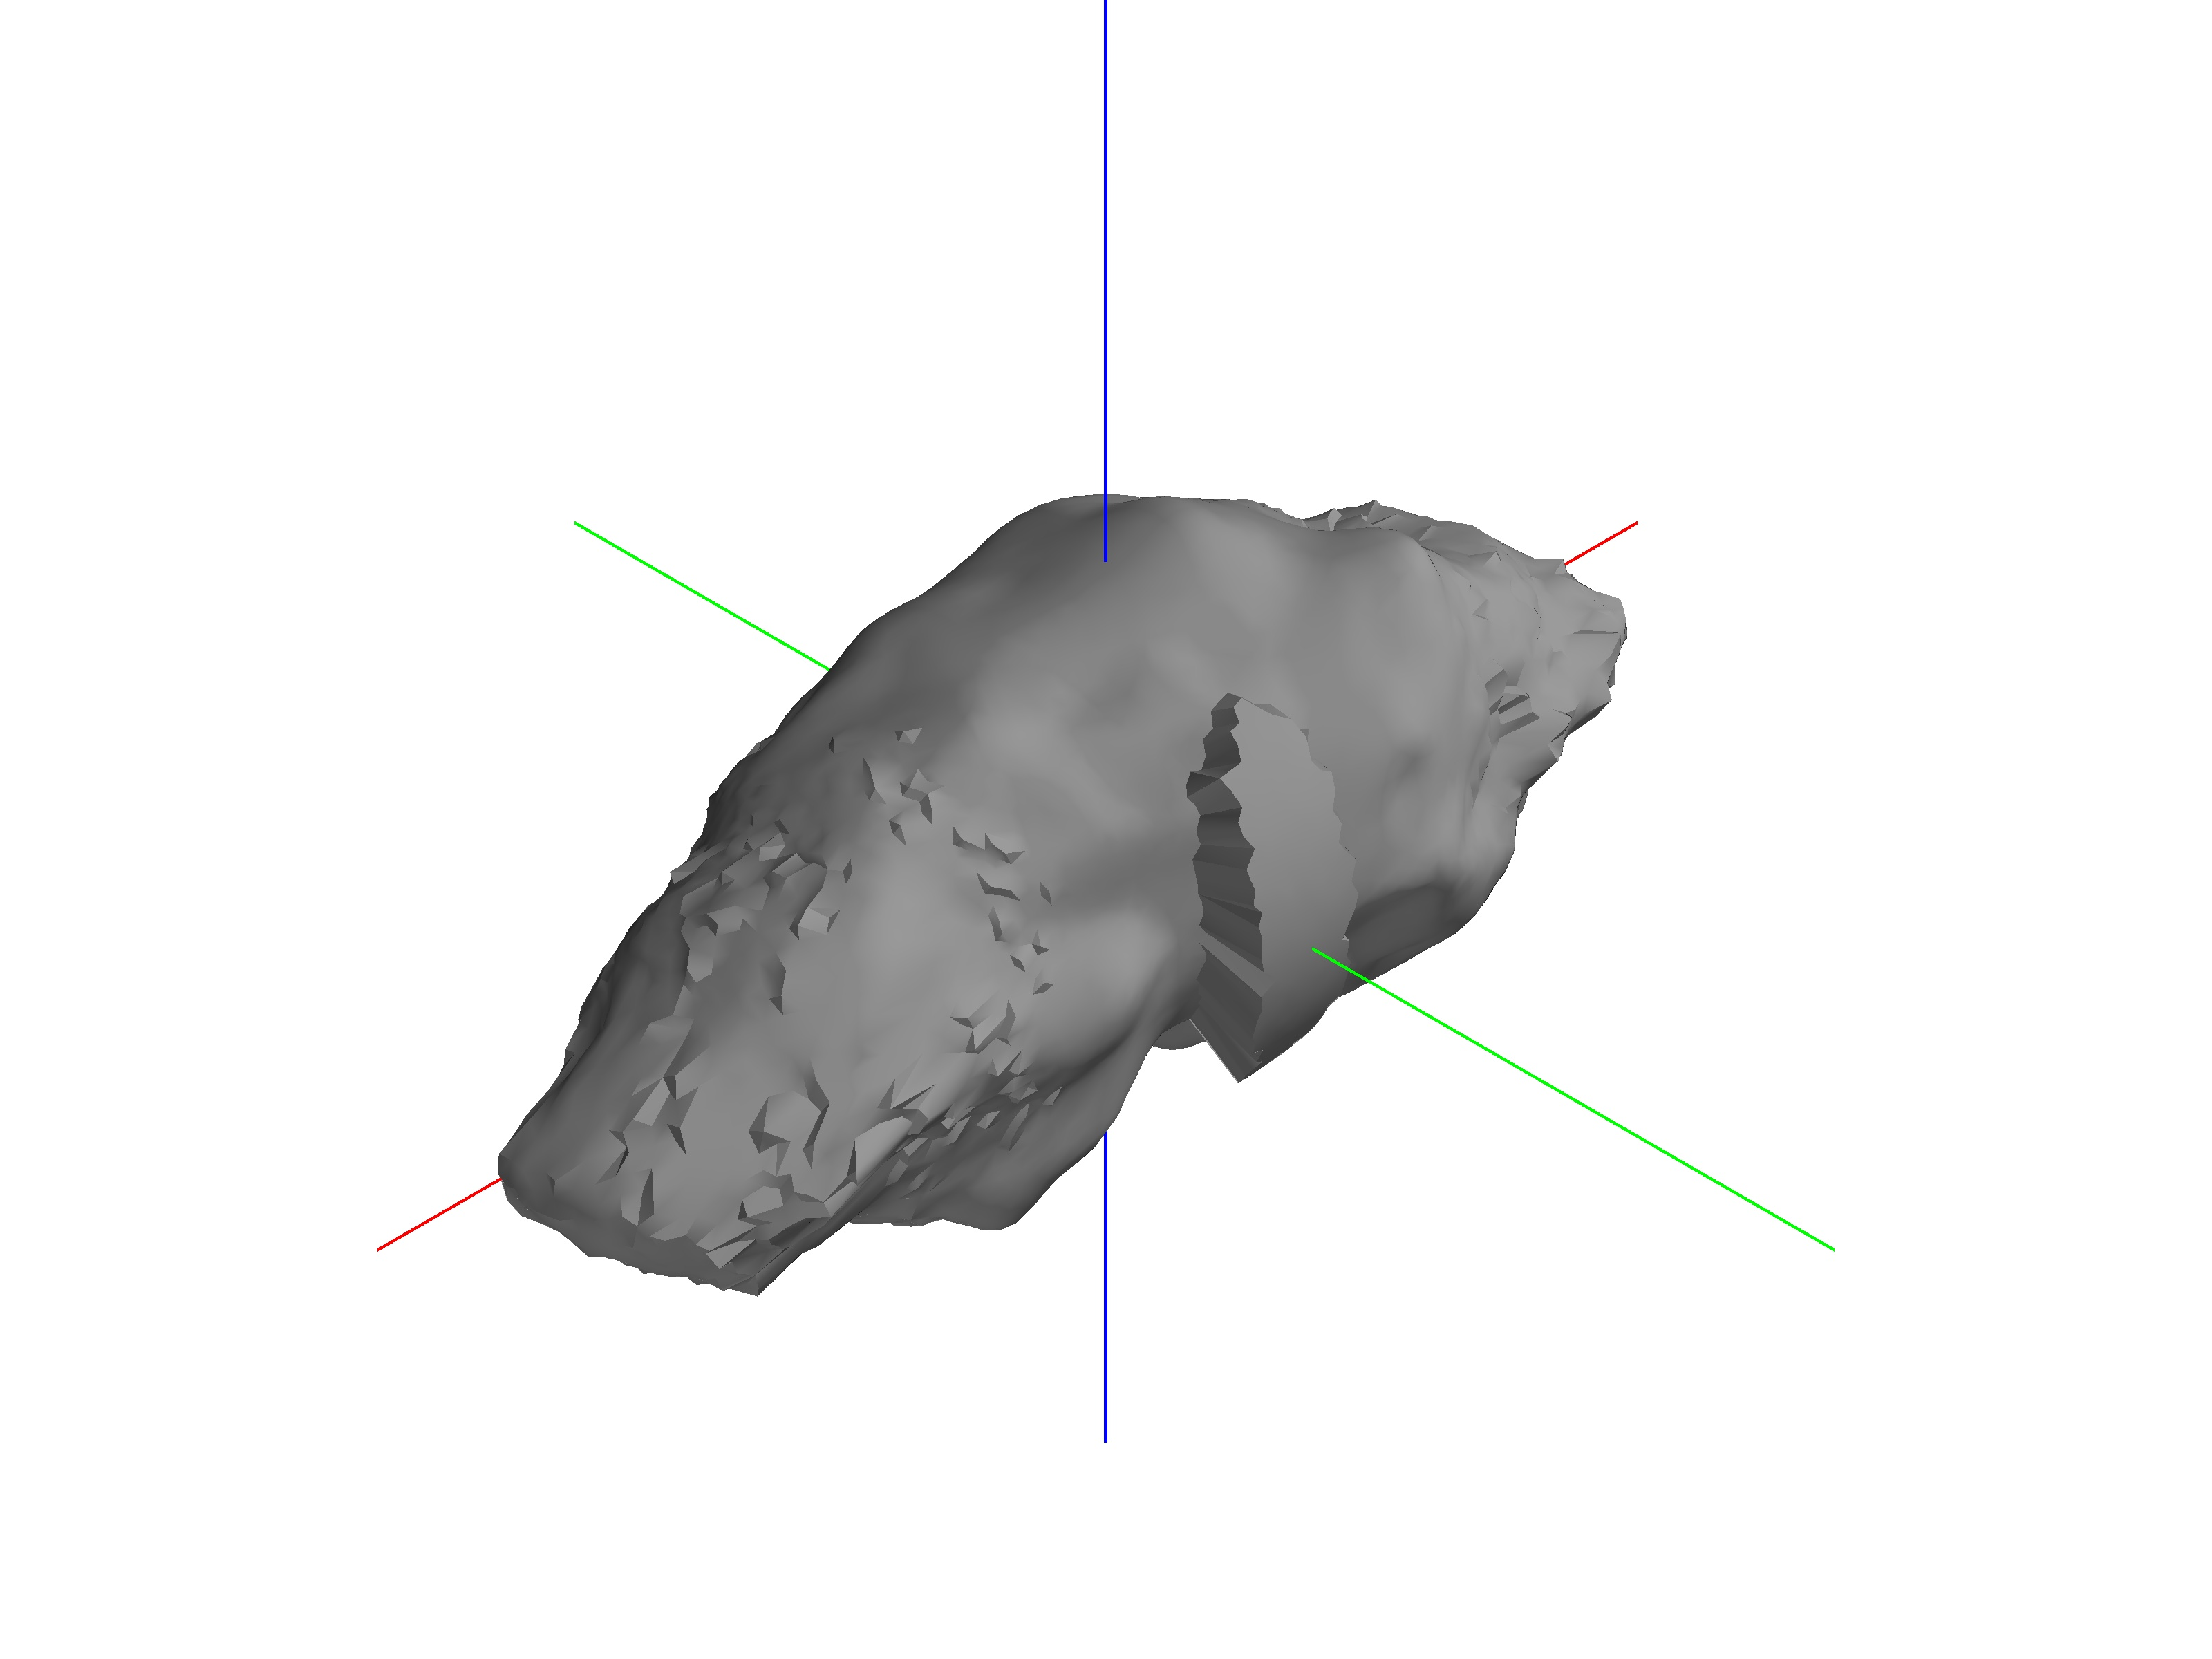
\includegraphics[trim={20cm 15cm 20cm 15cm},clip,keepaspectratio,width=0.5\textwidth]{figures/computational_geometry/mesh_update/geographos/partial_5617.jpg}}

    \subcaptionbox{\SI{100}{\percent} of measurements added\label{fig:geographos_partial_100}}{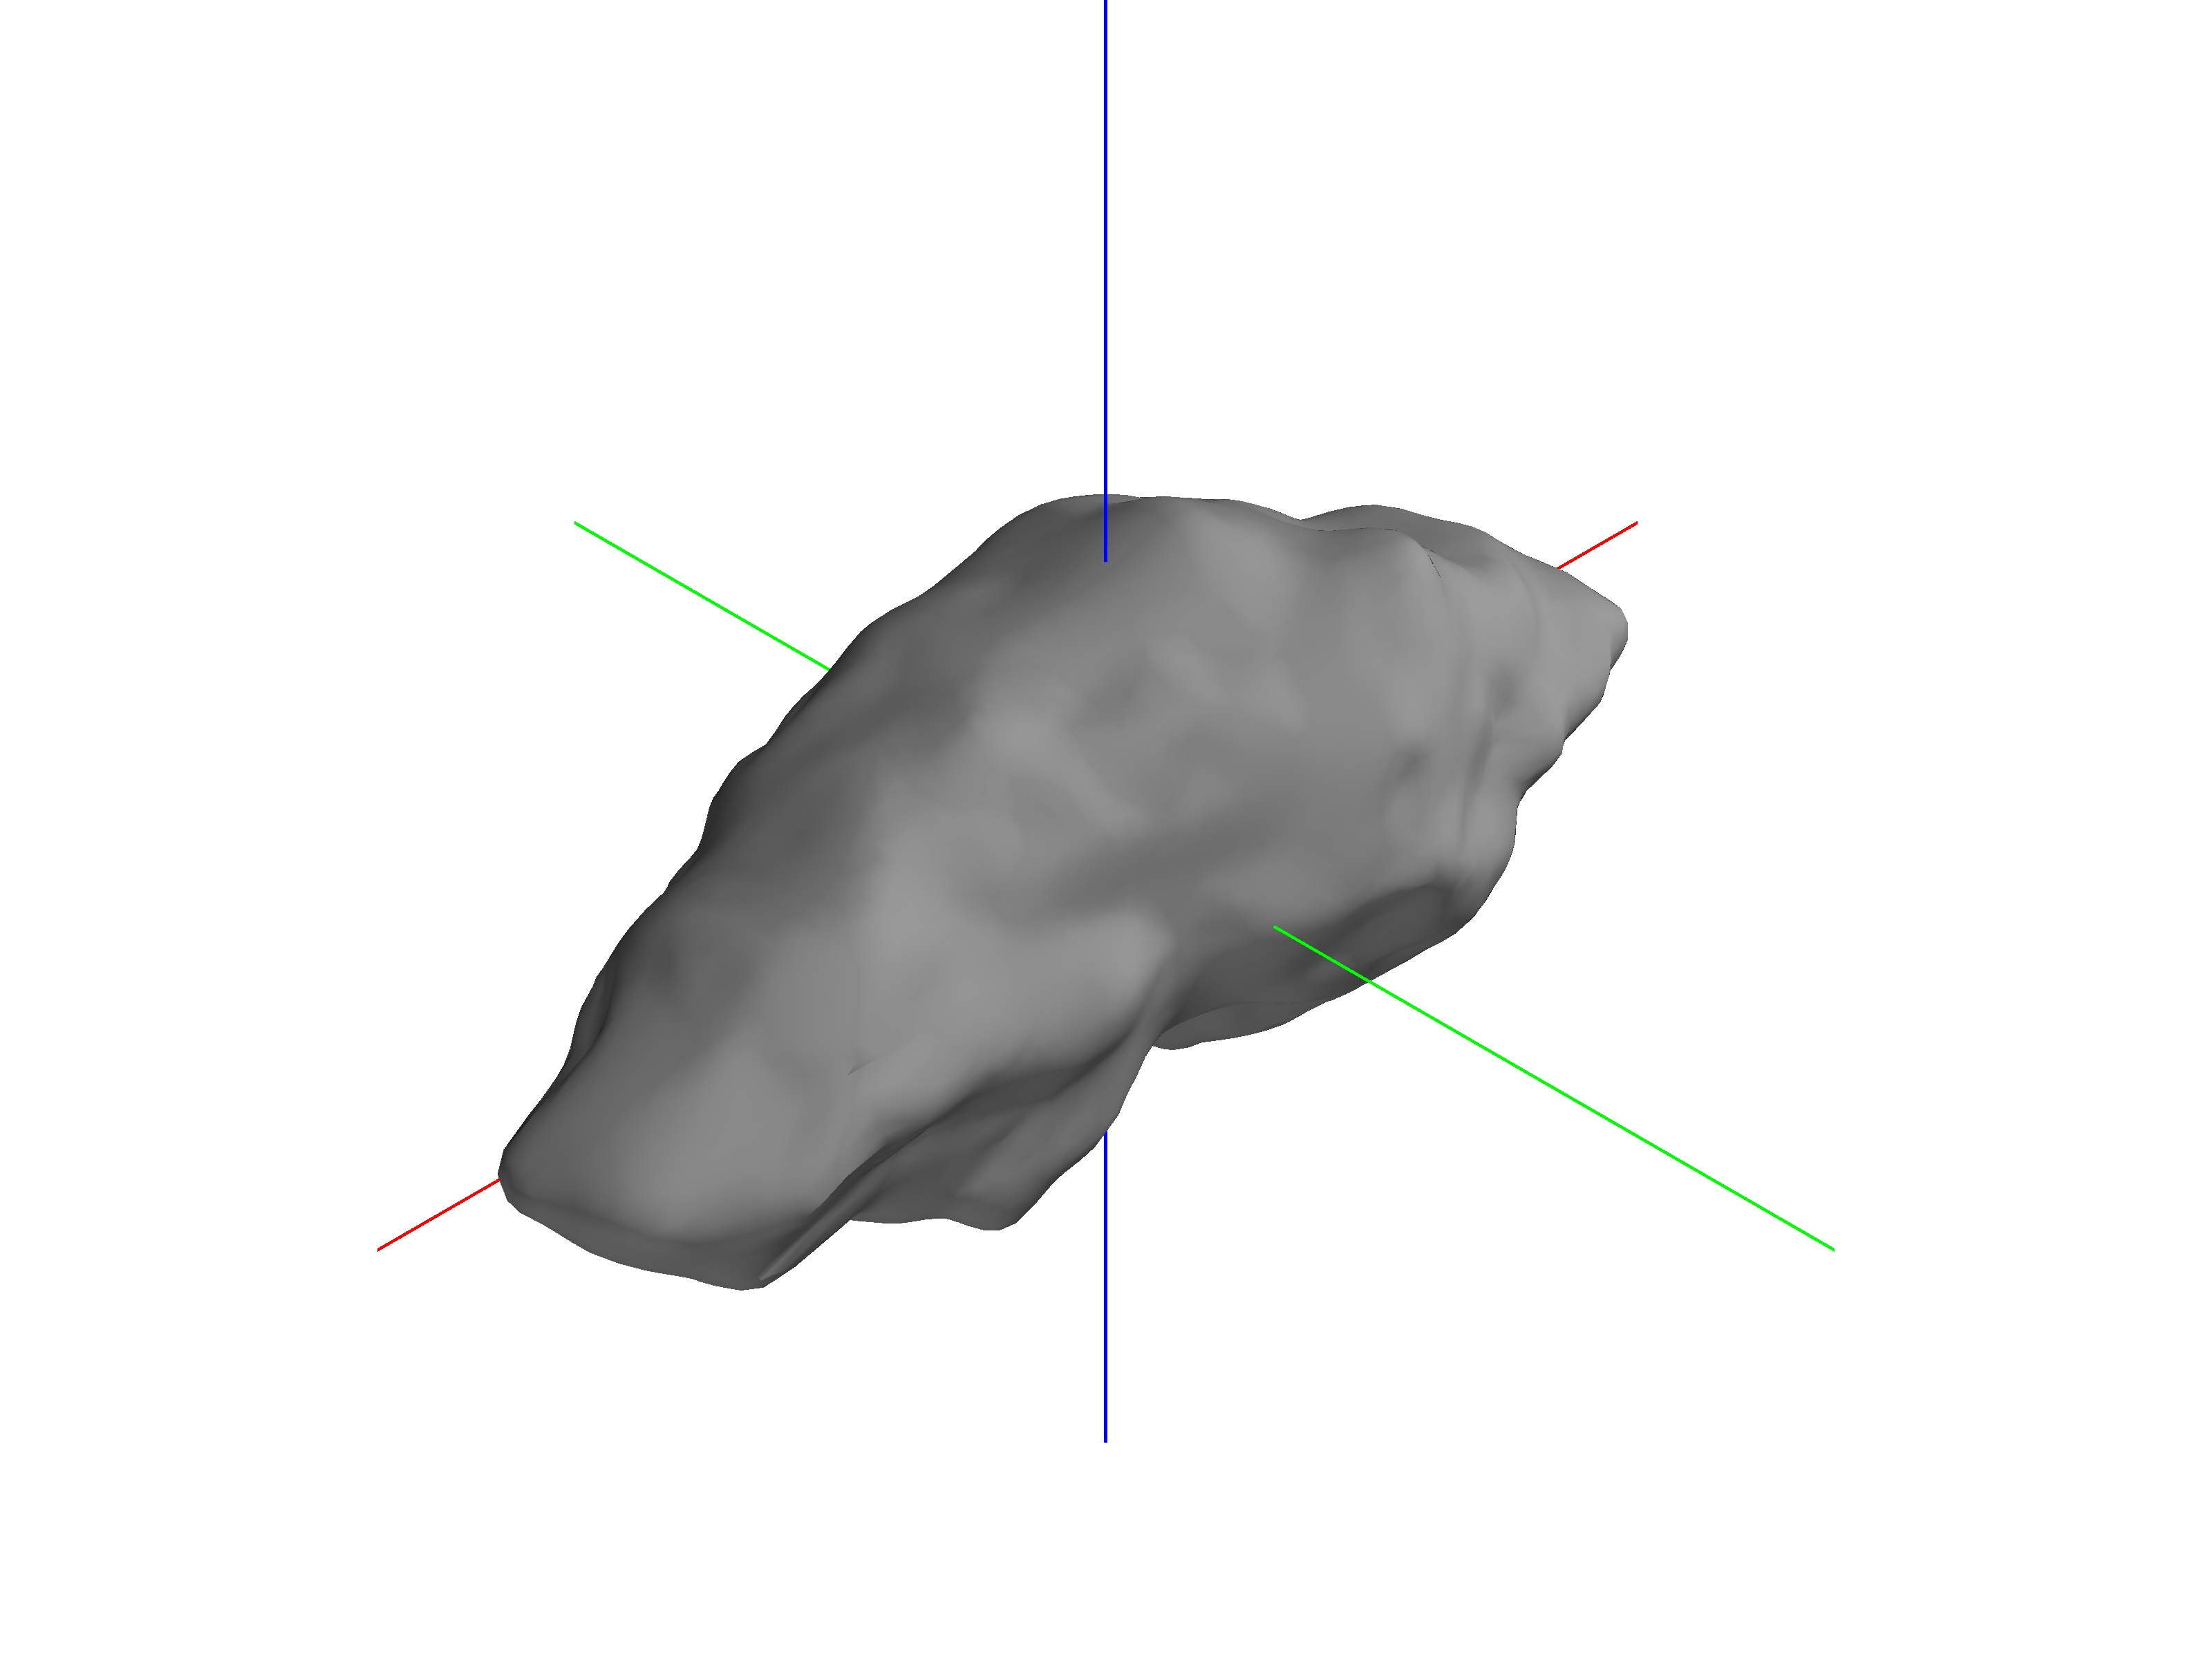
\includegraphics[trim={20cm 15cm 20cm 15cm},clip,keepaspectratio,width=0.5\textwidth]{figures/computational_geometry/mesh_update/geographos/partial_7489.jpg}}%
    \subcaptionbox{True Shape Model\label{fig:geographos_truth}}{\includegraphics[trim={20cm 15cm 20cm 15cm},clip,keepaspectratio,width=0.5\textwidth]{figures/computational_geometry/mesh_update/geographos/truth.jpg}}
    \caption[Asteroid Geographos incremental reconstruction]{Incremental reconstruction of asteroid Geographos~\label{fig:geographos_reconstruction}}
\end{figure}

\num{1620} Geographos is a highly elongated stony asteroid of the Apollo group.
Discovered in \num{1951}, Geographos is a potentially hazardous asteroid which passes sufficiently close to the Earth to present a hazard.
\Cref{fig:geographos_reconstruction} shows the shape reconstruction for asteroid Geographos at several distinct points during the process.
Comparing~\cref{fig:geographos_partial_100,fig:geographos_truth} shows that the final shape closely matches the true radar model.
In~\cref{fig:geographos_metrics} we display the vertex uncertainty and mesh volume as a function of time.
The plots show that the reconstruction achieves an accurate shape estimate with a total volume which closely matches the true volume.

\begin{figure}[htbp]
    \centering
    \tikzsetnextfilename{geographos_metrics}
\begin{tikzpicture}[baseline]
    \begin{groupplot}[
        group style={
            group name={geographos_metrics},
            group size=1 by 2,
            xlabels at=edge bottom,
            ylabels at=edge left,
            xticklabels at=edge bottom,
        },
        xlabel={Normalized Time},
        scale only axis,
        width=0.8\textwidth,
        height=0.1\textheight,
        ylabel style={align=center},
    ]
    \nextgroupplot[ylabel={Normalized\\Uncertainty}]
    \addplot [ultra thick, color=blue, mark=none] table [x=NORMALIZED_TIME, y=NORMALIZED_UNCERTAINTY, col sep=comma] {figures/mesh_update/geographos/uncertainty.csv};
    \addplot [ultra thick,red, mark=none, dashed] coordinates {
        (0.0, 0.0) (1.0, 0.0) 
    };

    \nextgroupplot[ylabel={Volume Percent\\Error}]
    \addplot [ultra thick, blue, mark=none] table [x=NORMALIZED_TIME, y=VOLUME_PERCENT_ERROR, col sep=comma] {figures/mesh_update/geographos/volume.csv};
        \addplot [ultra thick,red, mark=none, dashed] coordinates {
            (0.0, 0.0) (1.0, 0.0) 
        };
\end{groupplot}
\end{tikzpicture}


    \caption{Normalized uncertainty and volume percent error for Geographos\label{fig:geographos_metrics}}
\end{figure}

\num{6489} Golevka is a small angular shaped asteroid of the Apollo group.
Discovered in \num{1995}, Golevka is a potentially hazardous asteroid which passes sufficiently close to the Earth to present a hazard.
\Cref{fig:golevka_reconstruction} shows the shape reconstruction for asteroid Golevka at several distinct points during the process.
Comparing~\cref{fig:golevka_partial_100,fig:golevka_truth} shows that the final shape closely matches the true radar model.
In~\cref{fig:golevka_metrics} we display the vertex uncertainty and mesh volume as a function of time.

\begin{figure}[htbp]
    \centering
    \tikzsetnextfilename{golevka_metrics}
\begin{tikzpicture}[baseline]
    \begin{groupplot}[
        group style={
            group name={golevka_metrics},
            group size=1 by 2,
            xlabels at=edge bottom,
            ylabels at=edge left,
            xticklabels at=edge bottom,
        },
        xlabel={Normalized Time},
        scale only axis,
        width=0.8\textwidth,
        height=0.1\textheight,
        ylabel style={align=center},
    ]
    \nextgroupplot[ylabel={Normalized\\Uncertainty}]
    \addplot [ultra thick, color=blue, mark=none] table [x=NORMALIZED_TIME, y=NORMALIZED_UNCERTAINTY, col sep=comma] {figures/mesh_update/golevka/uncertainty.csv};
    \addplot [ultra thick,red, mark=none, dashed] coordinates {
        (0.0, 0.0) (1.0, 0.0) 
    };

    \nextgroupplot[ylabel={Volume Percent\\Error}]
    \addplot [ultra thick, blue, mark=none] table [x=NORMALIZED_TIME, y=VOLUME_PERCENT_ERROR, col sep=comma] {figures/mesh_update/golevka/volume.csv};
        \addplot [ultra thick,red, mark=none, dashed] coordinates {
            (0.0, 0.0) (1.0, 0.0) 
        };
\end{groupplot}
\end{tikzpicture}


    \caption{Normalized uncertainty and volume percent error for Golevka\label{fig:golevka_metrics}}
\end{figure}

The plots show that the reconstruction achieves an accurate shape estimate with a total volume which closely matches the true volume.
It is interesting to note that the reconstruction of Golevka achieves an accurate shape reconstruction in a much smaller amount of time as compared to Geographos.
This is primarily due to the smaller size of Golevka and the relatively spherical shape of the body in contrast to the highly elliptical shape of Geographos.

\begin{figure}[htbp]
    \centering
    \subcaptionbox{Initial Shape Estimate\label{fig:golevka_partial_0}}{\includegraphics[trim={20cm 5cm 20cm 5cm},clip,keepaspectratio,height=0.25\textheight]{figures/computational_geometry/mesh_update/golevka/partial_0.jpg}}%
    \subcaptionbox{\SI{25}{\percent} of measurements added\label{fig:golevka_partial_25}}{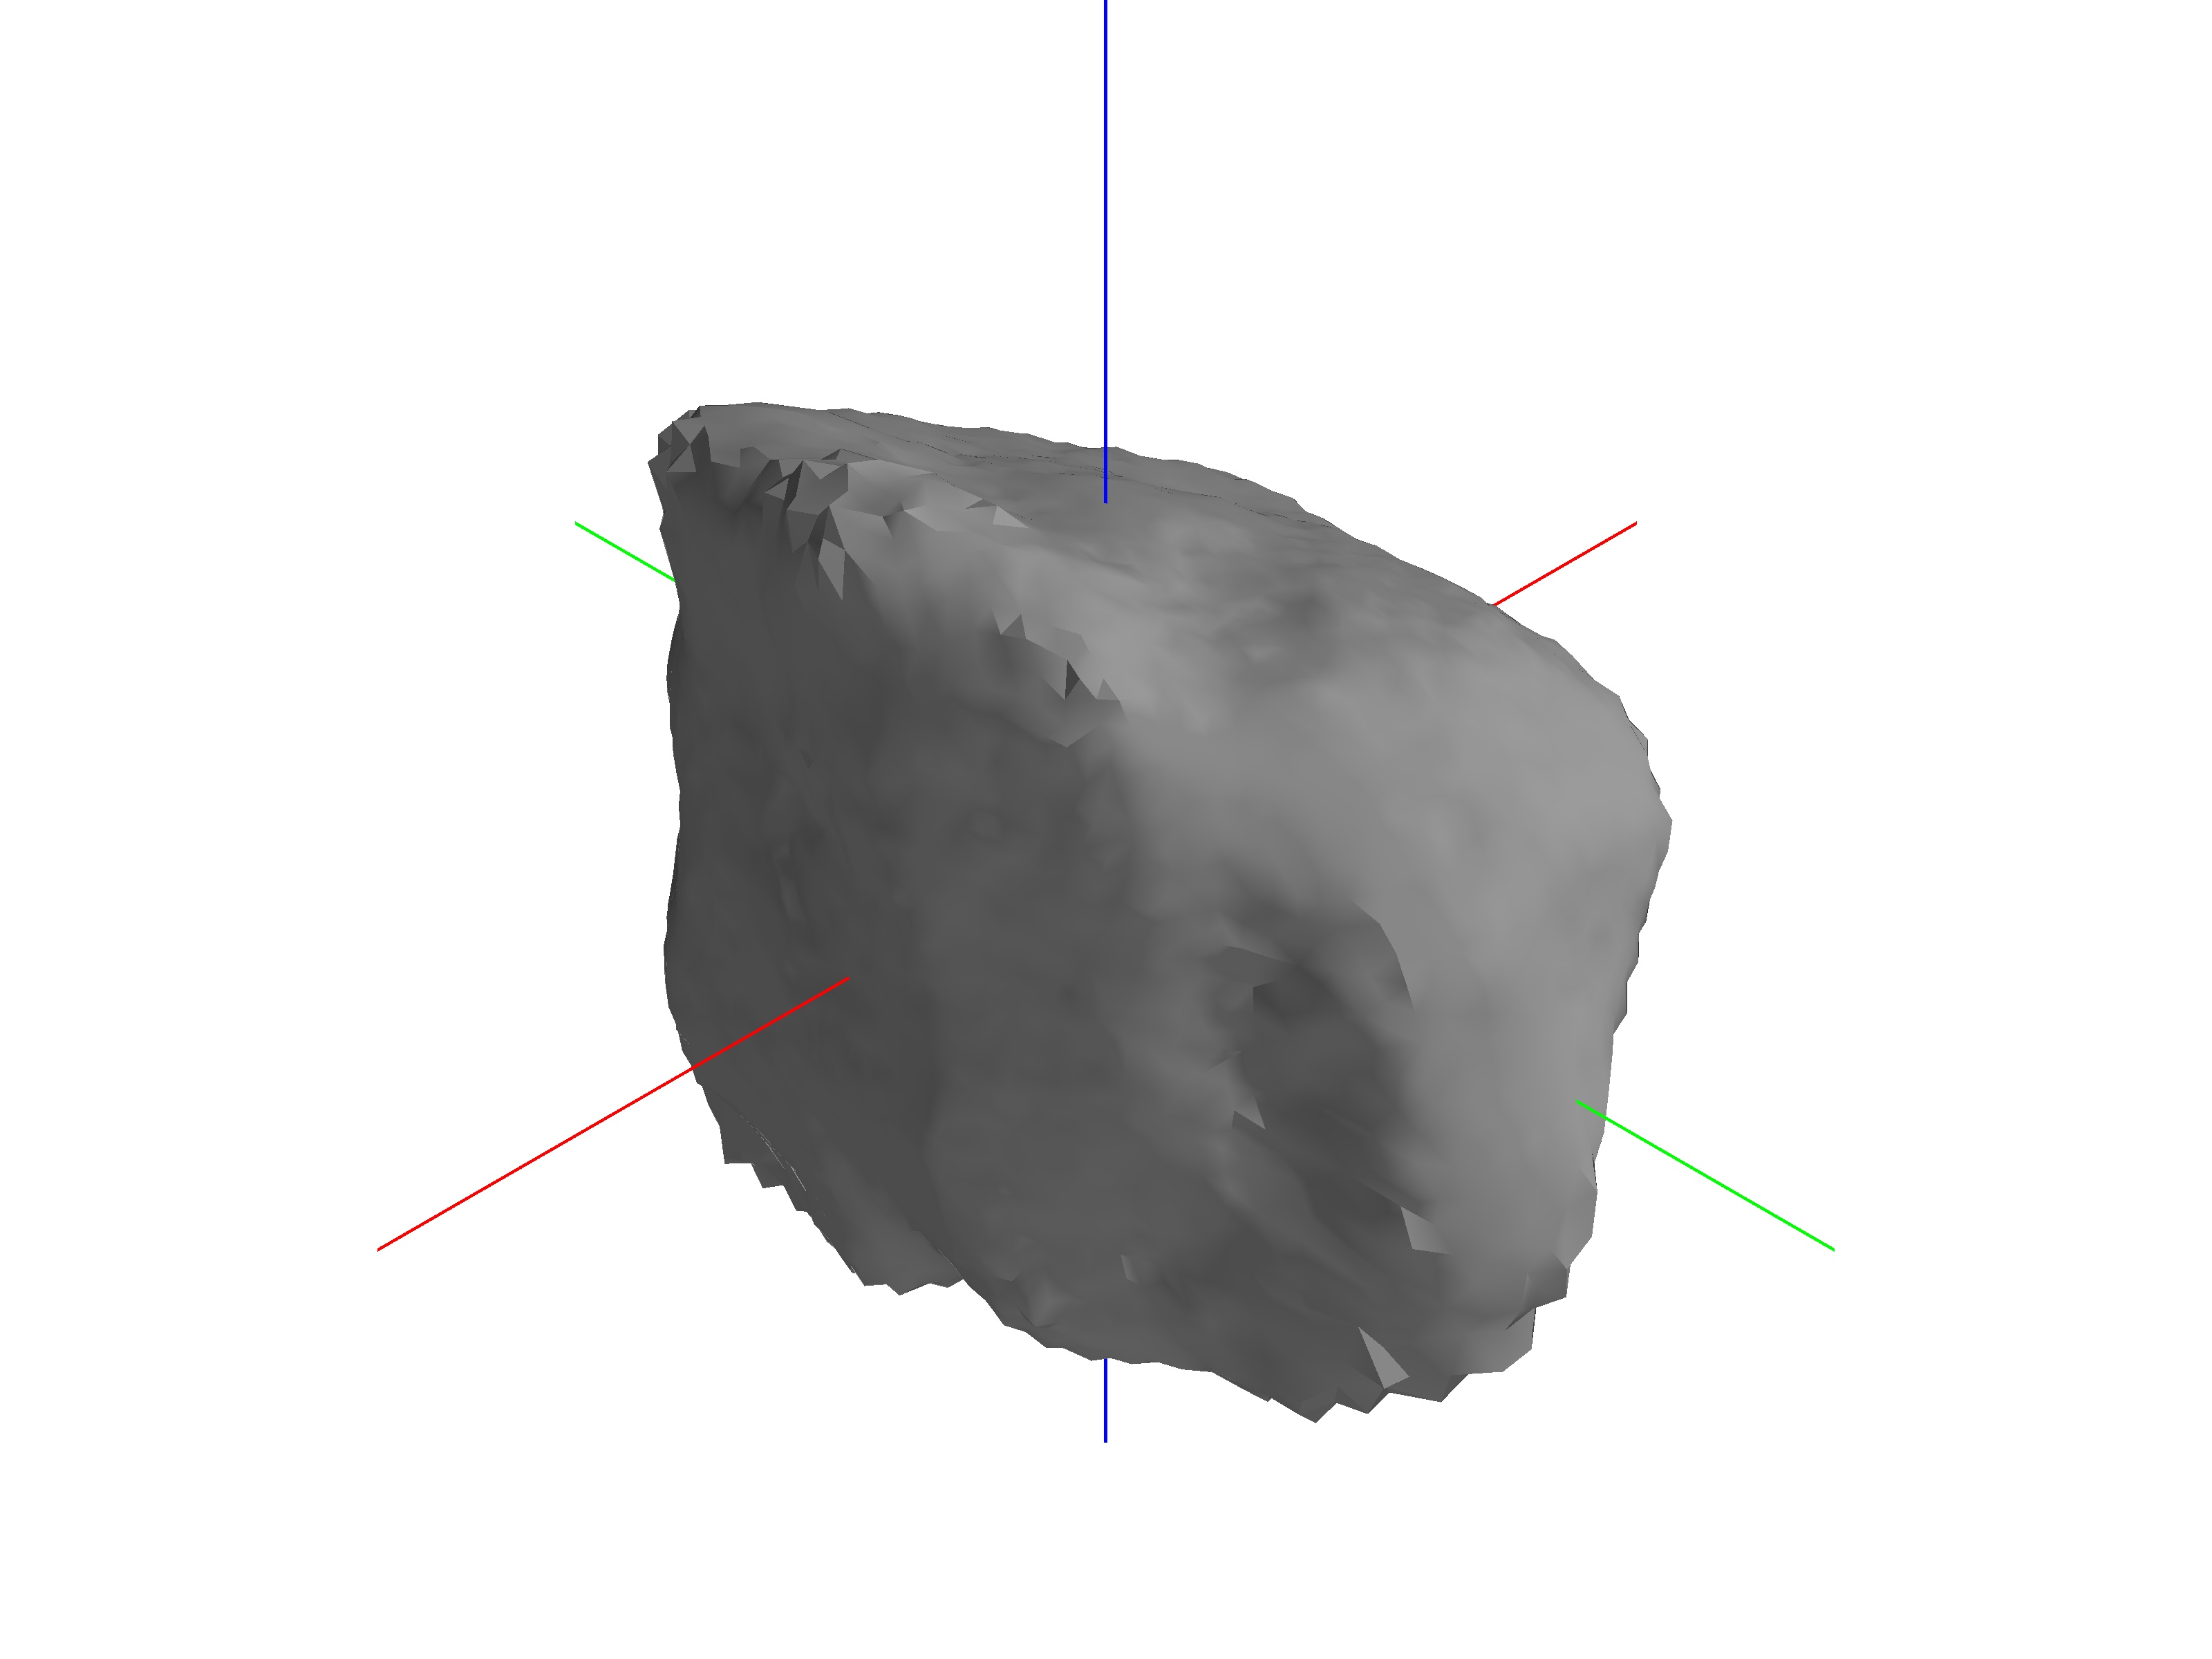
\includegraphics[trim={20cm 10cm 20cm 10cm},clip,keepaspectratio,height=0.25\textheight]{figures/computational_geometry/mesh_update/golevka/partial_1321.jpg}}\\%

    \subcaptionbox{\SI{50}{\percent} of measurements added\label{fig:golevka_partial_50}}{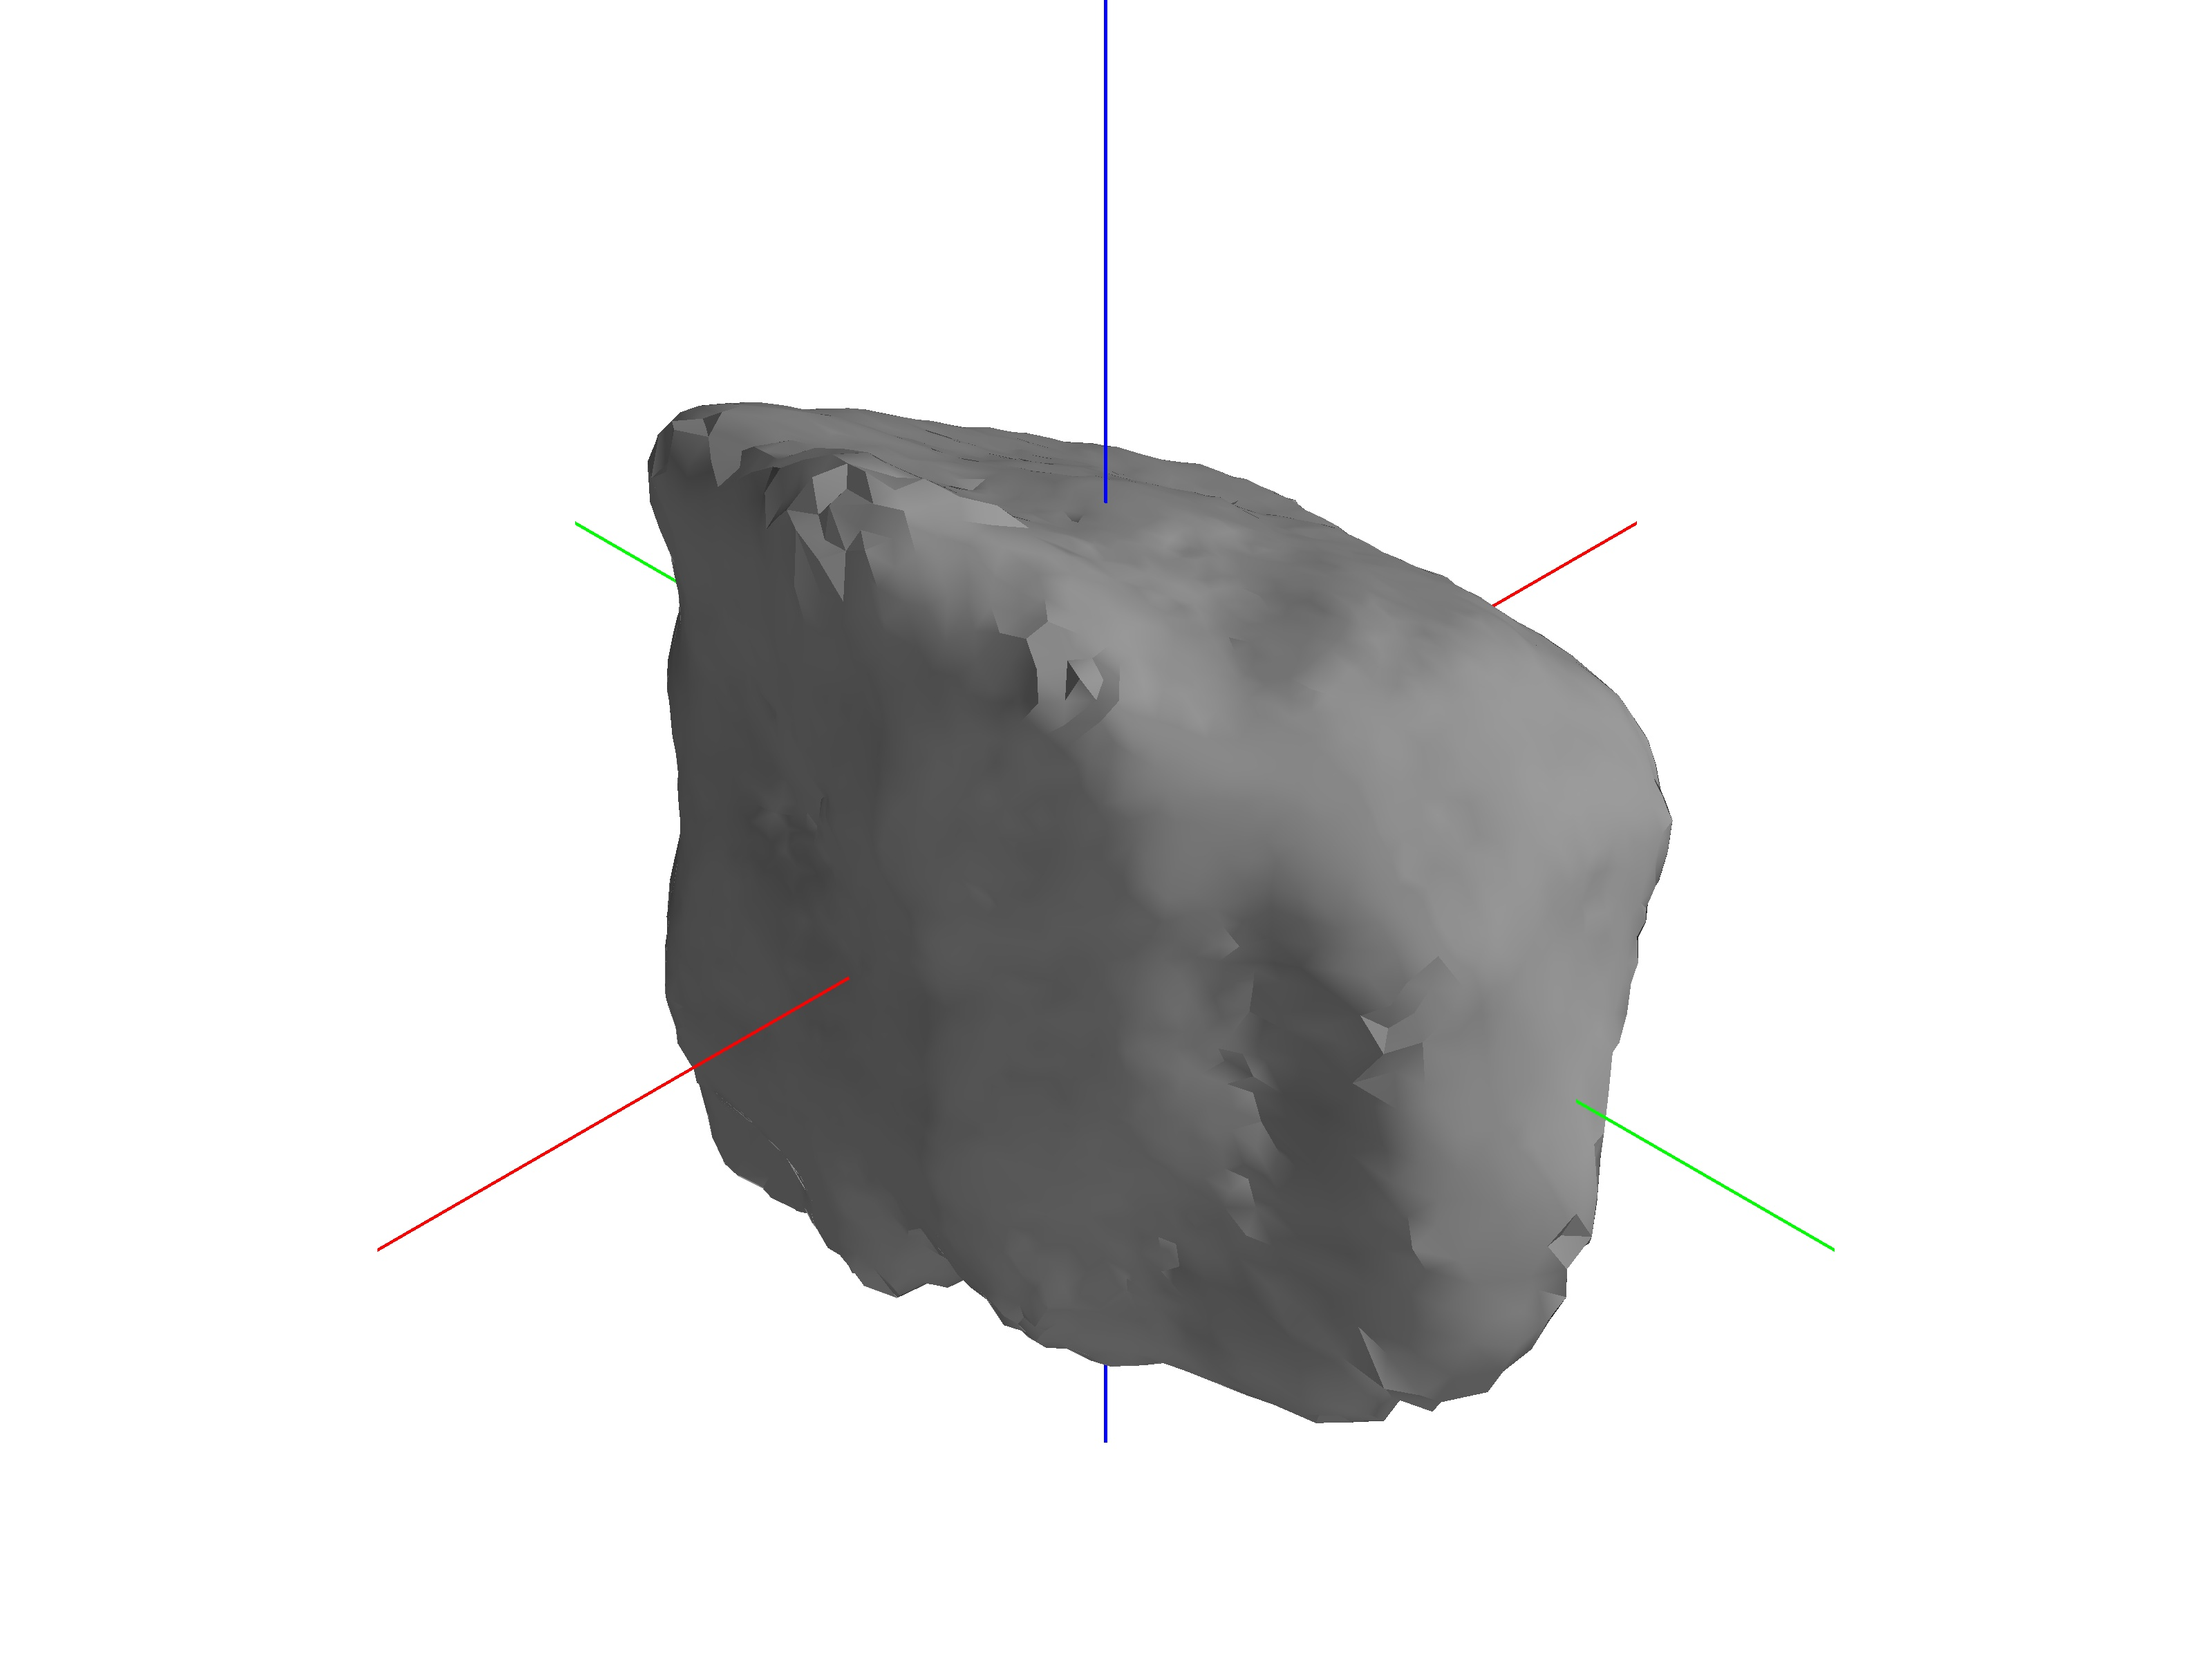
\includegraphics[trim={20cm 10cm 20cm 10cm},clip,keepaspectratio,height=0.25\textheight]{figures/computational_geometry/mesh_update/golevka/partial_2643.jpg}}%
    \subcaptionbox{\SI{75}{\percent} of measurements added\label{fig:golevka_partial_75}}{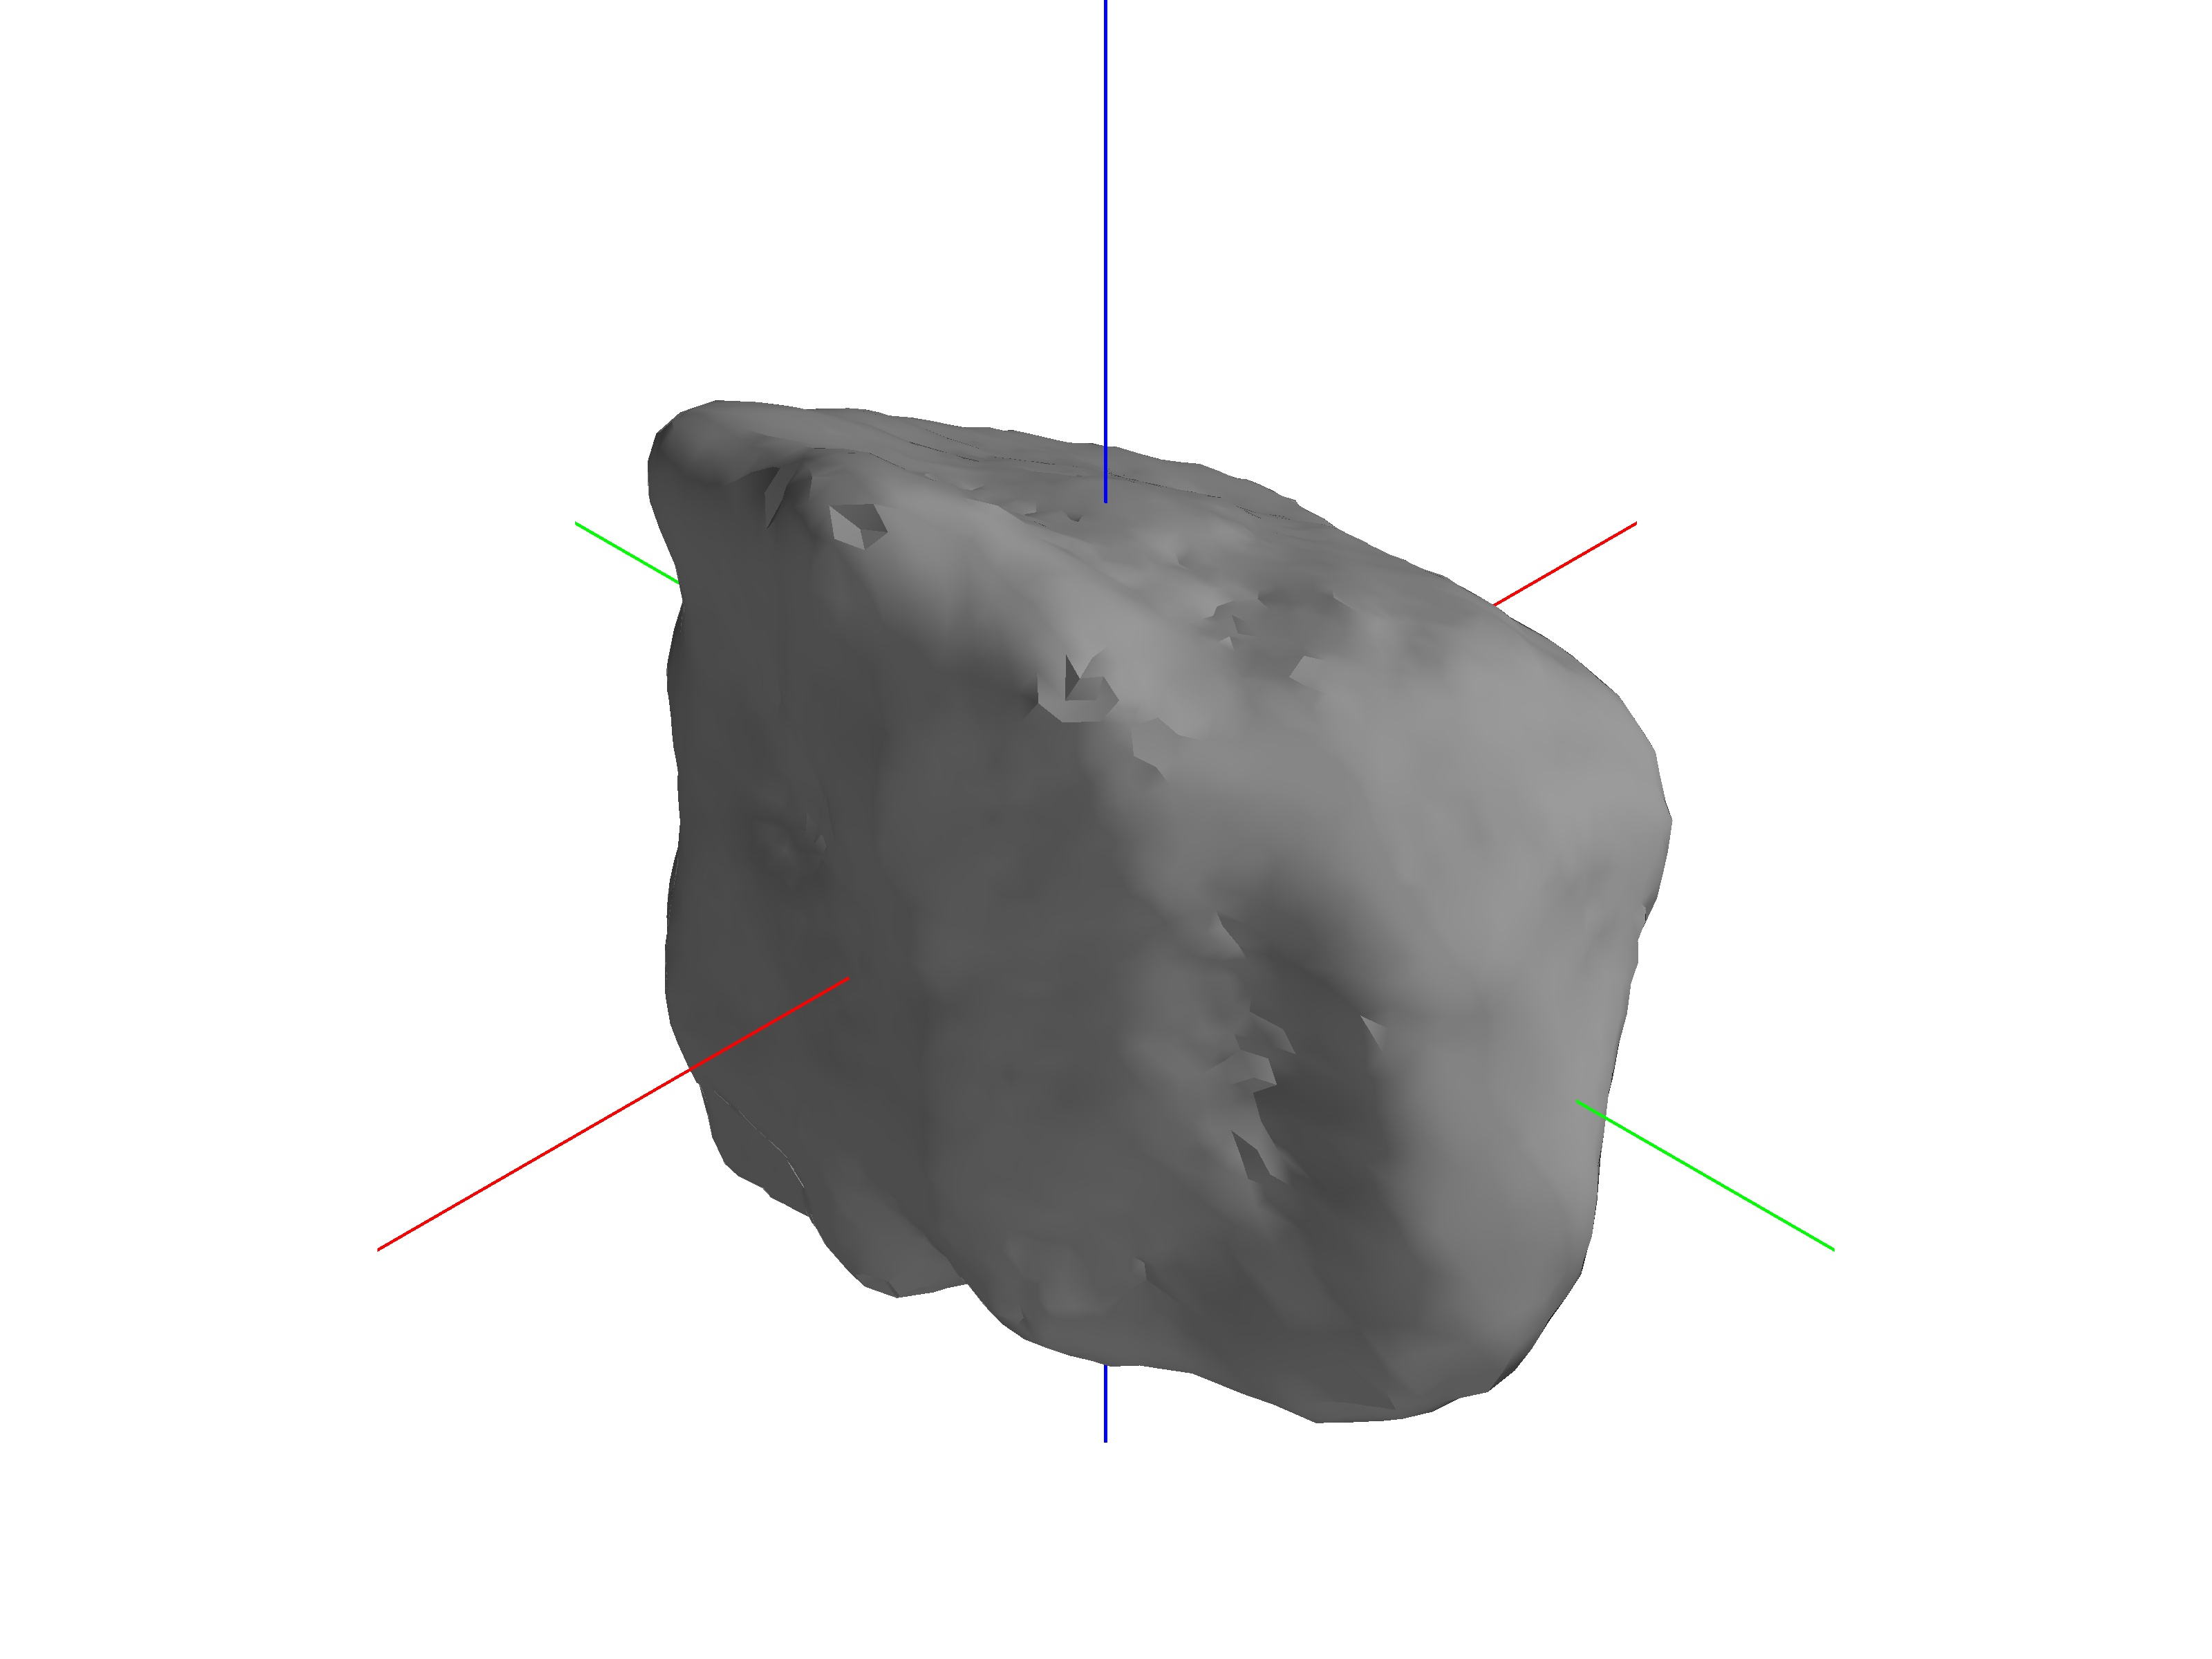
\includegraphics[trim={20cm 10cm 20cm 10cm},clip,keepaspectratio,height=0.25\textheight]{figures/computational_geometry/mesh_update/golevka/partial_3964.jpg}}\\%

    \subcaptionbox{\SI{100}{\percent} of measurements added\label{fig:golevka_partial_100}}{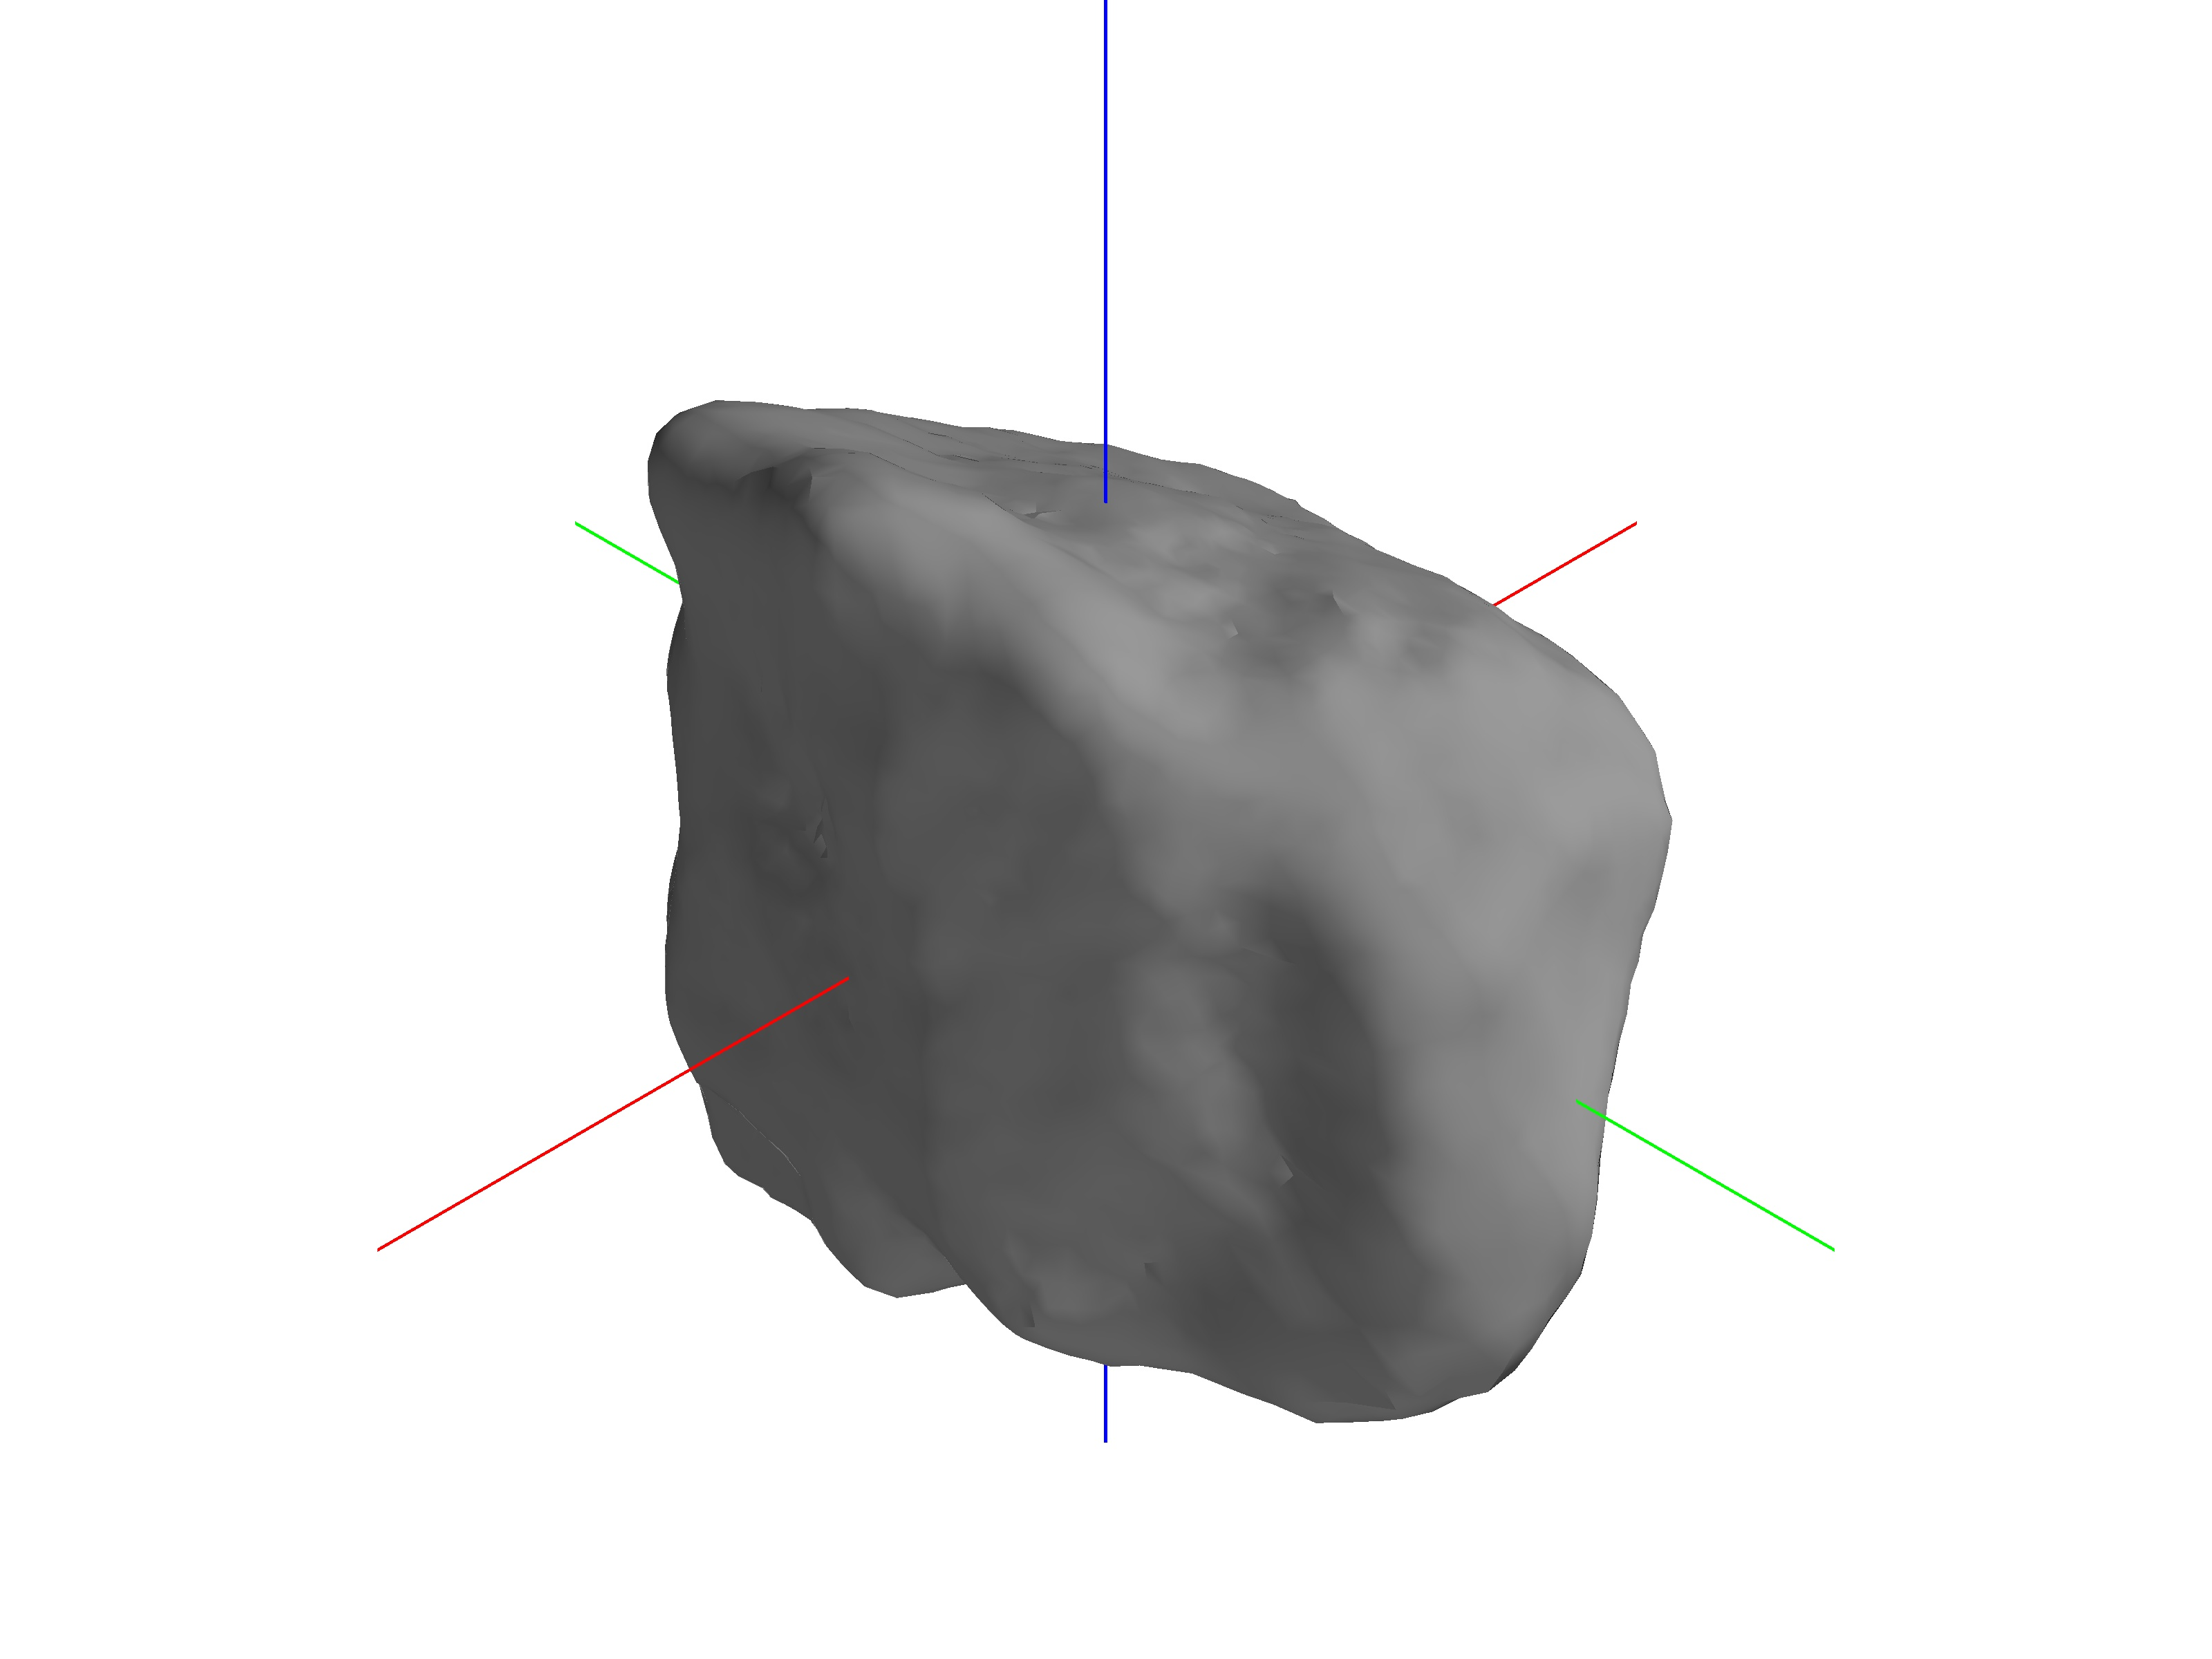
\includegraphics[trim={20cm 10cm 20cm 10cm},clip,keepaspectratio,height=0.25\textheight]{figures/computational_geometry/mesh_update/golevka/partial_5285.jpg}}%
    \subcaptionbox{True Shape Model\label{fig:golevka_truth}}{\includegraphics[trim={20cm 10cm 20cm 10cm},clip,keepaspectratio,height=0.25\textheight]{figures/computational_geometry/mesh_update/golevka/truth.jpg}}
    \caption[Asteroid Golevka incremental reconstruction]{Incremental reconstruction of asteroid Golevka~\label{fig:golevka_reconstruction}}
\end{figure}

\subsection{Full Dynamic Model }\label{sec:dynamic_exploration}

In this section, we simulate a dumbbell spacecraft in motion around asteroid \num{52760} and asteroid Castalia.
The dynamic simulation utilizes the inertial equations of motion from~\cref{sec:inertial_dumbbell_eoms} and are given as
\begin{align*}
    \dot{\ipos} &= \ivel, \\
    \parenth{m_1 + m_2} \dot{\ivel} &= - \sum_{i=0}^2 m_i \aatt \deriv{U}{\apos_i} + u_f, \\
    \dot{\iatt} &= \iatt \iangvel, \\
    J \dot{\iangvel} + \hat{\iangvel} J \iangvel &= \sum_{i=0}^2 m_i \hat{\spos}_i \iatt^T \aatt \deriv{U}{\apos_i} + u_m. 
\end{align*}
The nonlinear controllers described in~\cref{sec:se3_control} are used to control both the translational and rotational states of the vehicle.
The control inputs are duplicated from~\cref{sec:se3_control} as
\begin{align*}
    \vc{u}_f &= -k_x e_x - k_v e_v - F_{ext} + m \ddot{x}_d . \\
    \vc{u}_m &= -k_R e_R - k_\Omega e_\Omega + \Omega \times J \Omega - M_{ext}.
\end{align*}
Throughout the simulation the control inputs are computed using the current shape estimate of the asteroid. 
As measurements are collected, the spacecraft autonomously updates its shape estimate and uses this estimate to compute the control inputs and desired future states using the details provided in~\cref{sec:radius_update,sec:explore_asteroid}.
These simulations demonstrate the ability of a spacecraft to autonomously explore and maneuver around an unknown small body.

We consider two simulations about asteroids \num{52760} and Castalia.
The asteroids are assumed to constantly rotate about the \( \vc{f}_3 = \vc{e}_3\) axis according to the parameters given in~\cref{tab:dynamic_asteroids}.
Furthermore, the state of the asteroid, namely the rotation matrix \( \aatt \), is assumed to be known based on ground measurements or previous data.
\begin{table}[htbp]
    \centering
    \begin{tabular}{lcc}
        \toprule
        Property & \num{4769} Castalia & (\num{52760}) \num{1998} \(\text{ML}_{14}\) \\
        \midrule
        Semi-major axes(\si{\kilo\meter}) & \( 0.8065 \times 0.4905 \times 0.413 \) & \( 1.1 \times 1.1 \times 1.1 \) \\
        Rotational Period (\si{\hour}) & \num{4.095} & \num{14.98} \\
        Density (\si{\gram\per\centi\meter^3}) & \num{2.1} & \num{2.1} \\
        Vertices & \num{2048}  & \num{8192} \\
        Faces & \num{4092} & \num{16320} \\
        \bottomrule
    \end{tabular}
    \caption{Asteroid properties for dynamic exploration~\label{tab:dynamic_asteroids}}
\end{table}
At the beginning of the simulation the spacecraft is assumed to lie on the inertial \( e_1 \) axis, i.e.\ \( \ipos(0) = \begin{bmatrix} x_0 & 0 & 0 \end{bmatrix} \si{\kilo\meter} \).
In addition, at the initial state the spacecraft is orientated such that the \( b_1 \) axis is aligned with the inertial \( e_2 \) axis.
In other words the initial orientation is given by \( \iatt(0) = \exp(\frac{\pi}{2} \hat{e}_3)\).
The shape reconstruction phase of the simulation is performed over \SI{15000}{\second}, over which time the spacecraft will take \gls{lidar} measurements of the surface at \SI{1}{\hertz}.
Once the total uncertainty has been reduced sufficiently the spacecraft maneuvers to a ``home'' position aligned with the \( f_1 \) axis of the asteroid.

\paragraph{Asteroid 52760 Reconstruction}

Asteroid (\num{52760}) \num{1998} \(\text{ML}_{14}\) was discovered in \num{1998} and is near Earth asteroid of the Apollo group and classified as a potentially hazardous body.
The asteroid is roughly spherical with a mean radius of approximately \SI{1}{\kilo\meter}.
The initial shape estimate is assumed to be spherical with approximately the same number of vertices as the truth model.
\Cref{fig:52760_reconstruction,fig:52760_weights_reconstruction} show the shape reconstruction at several discrete points during the simulation.
Due to the roughly spherical shape of the asteroid large portions of the surface are quickly modified to match the measurements.
In addition~\cref{fig:52760_weights_reconstruction} displays the vertex uncertainty \( w_i \) as a colormap on the surface. 
Areas of high uncertainty are denoted in yellow while areas of low uncertainty are in purple/blue.

\begin{figure}[htbp]
    \centering
    \subcaptionbox{Initial Shape Estimate\label{fig:52760_partial_0}}{\includegraphics[trim={10cm 0cm 10cm 0cm},clip,height=0.25\textheight,width=0.5\textwidth,keepaspectratio]{figures/computational_geometry/dynamic_exploration/52760/partial_1.jpg}}%
    \subcaptionbox{\SI{25}{\percent} of measurements added\label{fig:52760_partial_25}}{\includegraphics[trim={10cm 0cm 10cm 0cm},clip,keepaspectratio,height=0.25\textheight]{figures/computational_geometry/dynamic_exploration/52760/partial_3749.jpg}}

    \subcaptionbox{\SI{50}{\percent} of measurements added\label{fig:52760_partial_50}}{\includegraphics[trim={10cm 0cm 10cm 0cm},clip,keepaspectratio,height=0.25\textheight]{figures/computational_geometry/dynamic_exploration/52760/partial_7499.jpg}}%
    \subcaptionbox{\SI{75}{\percent} of measurements added\label{fig:52760_partial_75}}{\includegraphics[trim={10cm 0cm 10cm 0cm},clip,keepaspectratio,height=0.25\textheight]{figures/computational_geometry/dynamic_exploration/52760/partial_11249.jpg}}

    \subcaptionbox{\SI{100}{\percent} of measurements added\label{fig:52760_partial_100}}{\includegraphics[trim={10cm 0cm 10cm 0cm},clip,keepaspectratio,height=0.25\textheight]{figures/computational_geometry/dynamic_exploration/52760/partial_14998.jpg}}%
    \subcaptionbox{True Shape Model\label{fig:52760_truth}}{\includegraphics[trim={10cm 0cm 10cm 0cm},clip,keepaspectratio,height=0.25\textheight]{figures/computational_geometry/mesh_update/52760/truth.jpg}}
    \caption[Asteroid 52760 incremental reconstruction]{Incremental reconstruction of asteroid 52760~\label{fig:52760_reconstruction}}
\end{figure}

\begin{figure}[htbp]
    \centering
    \subcaptionbox{Initial Shape Estimate\label{fig:52760_partial_weights_0}}{\includegraphics[trim={30cm 15cm 30cm 15cm},clip,height=0.25\textheight,width=0.5\textwidth,keepaspectratio]{figures/computational_geometry/dynamic_exploration/52760/partial_weights_1.jpg}}%
    \subcaptionbox{\SI{25}{\percent} of measurements added\label{fig:52760_partial_weights_25}}{\includegraphics[trim={30cm 15cm 30cm 15cm},clip,height=0.25\textheight,width=0.5\textwidth,keepaspectratio]{figures/computational_geometry/dynamic_exploration/52760/partial_weights_3749.jpg}}

    \subcaptionbox{\SI{50}{\percent} of measurements added\label{fig:52760_partial_weights_50}}{\includegraphics[trim={30cm 15cm 30cm 15cm},clip,height=0.25\textheight,width=0.5\textwidth,keepaspectratio]{figures/computational_geometry/dynamic_exploration/52760/partial_weights_7499.jpg}}%
    \subcaptionbox{\SI{75}{\percent} of measurements added\label{fig:52760_partial_weights_75}}{\includegraphics[trim={30cm 15cm 30cm 15cm},clip,height=0.25\textheight,width=0.5\textwidth,keepaspectratio]{figures/computational_geometry/dynamic_exploration/52760/partial_weights_11249.jpg}}

    \subcaptionbox{\SI{100}{\percent} of measurements added\label{fig:52760_partial_weights_100}}{\includegraphics[trim={30cm 15cm 30cm 15cm},clip,height=0.25\textheight,width=0.5\textwidth,keepaspectratio]{figures/computational_geometry/dynamic_exploration/52760/partial_weights_14998.jpg}}%
    % \subcaptionbox{True Shape Model\label{fig:52760_weights_truth}}{\includegraphics[trim={15cm 0cm 15cm 5cm},clip,height=0.18\textheight,width=0.5\textwidth,keepaspectratio]{figures/computational_geometry/mesh_update/52760/truth.jpg}}
    \caption[Asteroid 52760 shape reconstruction with uncertainty]{Incremental reconstruction of asteroid 52760. The images colored according to the shape uncertainty. Areas of high uncertainty are in yellow while ares of low uncertainty are in purple.~\label{fig:52760_weights_reconstruction}}
\end{figure}
\Cref{fig:52760_metrics} shows the total normalized uncertainty and percent error for the volume estimate. 
The plots show that the reconstruction  converges to an accurate shape estimate after approximately \SI{8000}{\second}.

\begin{figure}[htbp]
    \centering
    \tikzsetnextfilename{52760_metrics}
\begin{tikzpicture}[baseline]
    \begin{groupplot}[
        group style={
            group name={52760_metrics},
            group size=1 by 2,
            xlabels at=edge bottom,
            ylabels at=edge left,
            xticklabels at=edge bottom,
        },
        xlabel={Normalized Time},
        scale only axis,
        width=0.8\textwidth,
        height=0.1\textheight,
        ylabel style={align=center},
    ]
    \nextgroupplot[ylabel={Normalized\\Uncertainty}]
    \addplot [ultra thick, color=blue, mark=none] table [x=NORMALIZED_TIME, y=NORMALIZED_UNCERTAINTY, col sep=comma] {figures/dynamic_exploration/52760/uncertainty.csv};
    \addplot [ultra thick,red, mark=none, dashed] coordinates {
        (0.0, 0.0) (1.0, 0.0) 
    };

    \nextgroupplot[ylabel={Volume Percent\\Error}]
    \addplot [ultra thick, blue, mark=none] table [x=NORMALIZED_TIME, y=VOLUME_PERCENT_ERROR, col sep=comma] {figures/dynamic_exploration/52760/volume.csv};
        \addplot [ultra thick,red, mark=none, dashed] coordinates {
            (0.0, 0.0) (1.0, 0.0) 
        };
\end{groupplot}
\end{tikzpicture}


    \caption{Normalized uncertainty and volume percent error for 52760\label{fig:52760_metrics}}
\end{figure}

\begin{figure}[htbp]
    \centering
    \subcaptionbox{3D visualization of the trajectory\label{fig:52760_explore_trajectory}}{\includegraphics[trim={0 0 0 0},clip,keepaspectratio,width=0.99\textwidth]{figures/computational_geometry/dynamic_exploration/52760/state/asteroid_trajectory.jpg}
}\\%
    \subcaptionbox{Components of position\label{fig:52760_explore_components}}{\tikzsetnextfilename{52760_ast_comp}
\begin{tikzpicture}[baseline]
    \begin{groupplot}[
        group style={
            group name={52760_ast_comp},
            group size=1 by 3,
            xlabels at=edge bottom,
            ylabels at=edge left,
            xticklabels at=edge bottom,
            vertical sep=0pt,
        },
        xlabel={Normalized Time},
        scale only axis,
        width=0.8\textwidth,
        height=0.1\textheight,
    ]
    \nextgroupplot[ylabel={$ x$}]
    \addplot [ultra thick,blue, mark=none] table [x=NORMALIZED_TIME, y=ASTEROID_X, col sep=comma] {figures/dynamic_exploration/52760/state/state_trajectory.csv};

    \nextgroupplot[ylabel={$ y  $}]
    \addplot [ultra thick,blue, mark=none] table [x=NORMALIZED_TIME, y=ASTEROID_Y, col sep=comma] {figures/dynamic_exploration/52760/state/state_trajectory.csv};

    \nextgroupplot[ylabel={$ z  $}]
    \addplot [ultra thick,blue, mark=non] table [x=NORMALIZED_TIME, y=ASTEROID_Z, col sep=comma] {figures/dynamic_exploration/52760/state/state_trajectory.csv};

\end{groupplot}
\end{tikzpicture}
}
    \caption{Spacecraft trajectory in the rotating asteroid frame for the exploration of 52760~\label{fig:52760_trajectory}}
\end{figure}

\paragraph{Asteroid 4769 Castalia Reconstruction}

Asteroid 4769 Castalia is a small near Earth asteroid of the Apollo group.
In addition, it is classified as a potentially hazardous object with a closed approach distance of less than \SI{0.05}{\astronomicalunit}.
Castalia was discovered in \num{1989} and is the first asteroid to be modeled using radar imagery~\cite{hudson1994}.
Castalia is composed of two distinct lobes suggesting that it is a contact binary of two smaller objects held together by their mutual gravity.
\Cref{fig:castalia_reconstruction,fig:castalia_weights_reconstruction} show the shape reconstruction at several discrete points during the simulation.
In addition~\cref{fig:castalia_weights_reconstruction} displays the vertex uncertainty \( w_i \) as a colormap on the surface. 
Areas of high uncertainty are denoted in yellow while areas of low uncertainty are in purple/blue.
Within \SI{50}{\percent} of the simulation span the spacecraft is able to achieve an accurate estimate of the true shape of Castalia.

\begin{figure}[htbp]
    \centering
    \subcaptionbox{Initial Shape Estimate\label{fig:castalia_partial_0}}{\includegraphics[trim={15cm 10cm 15cm 10cm},clip,height=0.5\textheight,width=0.5\textwidth,keepaspectratio]{figures/computational_geometry/dynamic_exploration/castalia/partial_1.jpg}}%
    \subcaptionbox{\SI{25}{\percent} of measurements added\label{fig:castalia_partial_25}}{\includegraphics[trim={15cm 10cm 15cm 10cm},clip,height=0.5\textheight,width=0.5\textwidth,keepaspectratio]{figures/computational_geometry/dynamic_exploration/castalia/partial_3749.jpg}}

    \subcaptionbox{\SI{50}{\percent} of measurements added\label{fig:castalia_partial_50}}{\includegraphics[trim={15cm 10cm 15cm 10cm},clip,height=0.5\textheight,width=0.5\textwidth,keepaspectratio]{figures/computational_geometry/dynamic_exploration/castalia/partial_7499.jpg}}%
    \subcaptionbox{\SI{75}{\percent} of measurements added\label{fig:castalia_partial_75}}{\includegraphics[trim={15cm 10cm 15cm 10cm},clip,height=0.5\textheight,width=0.5\textwidth,keepaspectratio]{figures/computational_geometry/dynamic_exploration/castalia/partial_11249.jpg}}

    \subcaptionbox{\SI{100}{\percent} of measurements added\label{fig:castalia_partial_100}}{\includegraphics[trim={15cm 10cm 15cm 10cm},clip,height=0.5\textheight,width=0.5\textwidth,keepaspectratio]{figures/computational_geometry/dynamic_exploration/castalia/partial_14998.jpg}}%
    \subcaptionbox{True Shape Model\label{fig:castalia_truth}}{\includegraphics[trim={15cm 10cm 15cm 10cm},clip,height=0.5\textheight,width=0.5\textwidth,keepaspectratio]{figures/computational_geometry/mesh_update/castalia/truth.jpg}}
    \caption[Asteroid Castalia incremental reconstruction]{Incremental reconstruction of asteroid Castalia~\label{fig:castalia_reconstruction}}
\end{figure}

\begin{figure}[htbp]
    \centering
    \subcaptionbox{Initial Shape Estimate\label{fig:castalia_partial_weights_0}}{\includegraphics[trim={15cm 10cm 15cm 10cm},clip,height=0.5\textheight,width=0.5\textwidth,keepaspectratio]{figures/computational_geometry/dynamic_exploration/castalia/partial_weights_1.jpg}}%
    \subcaptionbox{\SI{25}{\percent} of measurements added\label{fig:castalia_partial_weights_25}}{\includegraphics[trim={15cm 10cm 15cm 10cm},clip,height=0.5\textheight,width=0.5\textwidth,keepaspectratio]{figures/computational_geometry/dynamic_exploration/castalia/partial_weights_3749.jpg}}

    \subcaptionbox{\SI{50}{\percent} of measurements added\label{fig:castalia_partial_weights_50}}{\includegraphics[trim={15cm 10cm 15cm 10cm},clip,height=0.5\textheight,width=0.5\textwidth,keepaspectratio]{figures/computational_geometry/dynamic_exploration/castalia/partial_weights_7499.jpg}}%
    \subcaptionbox{\SI{75}{\percent} of measurements added\label{fig:castalia_partial_weights_75}}{\includegraphics[trim={15cm 10cm 15cm 10cm},clip,height=0.5\textheight,width=0.5\textwidth,keepaspectratio]{figures/computational_geometry/dynamic_exploration/castalia/partial_weights_11249.jpg}}

    \subcaptionbox{\SI{100}{\percent} of measurements added\label{fig:castalia_partial_weights_100}}{\includegraphics[trim={15cm 10cm 15cm 10cm},clip,height=0.5\textheight,width=0.5\textwidth,keepaspectratio]{figures/computational_geometry/dynamic_exploration/castalia/partial_weights_14998.jpg}}%
    \subcaptionbox{True Shape Model\label{fig:castalia_weights_truth}}{\includegraphics[trim={15cm 10cm 15cm 10cm},clip,height=0.5\textheight,width=0.5\textwidth,keepaspectratio]{figures/computational_geometry/mesh_update/castalia/truth.jpg}}
    \caption[Asteroid Castalia shape reconstruction with uncertainty]{Incremental reconstruction of asteroid Castalia. The images colored according to the shape uncertainty. Areas of high uncertainty are in yellow while ares of low uncertainty are in purple.~\label{fig:castalia_weights_reconstruction}}
\end{figure}

\Cref{fig:castalia_metrics} shows the total normalized uncertainty and percent error for the volume estimate. 
The plots show that the reconstruction converges to an accurate shape estimate after approximately \SI{8000}{\second}.
In addition, the volume estimate is initially a much larger value but quickly converges to the true value.
\begin{figure}[htbp]
    \centering
    \tikzsetnextfilename{castalia_metrics}
\begin{tikzpicture}[baseline]
    \begin{groupplot}[
        group style={
            group name={castalia_metrics},
            group size=1 by 2,
            xlabels at=edge bottom,
            ylabels at=edge left,
            xticklabels at=edge bottom,
        },
        xlabel={Normalized Time},
        scale only axis,
        width=0.8\textwidth,
        height=0.1\textheight,
        ylabel style={align=center},
    ]
    \nextgroupplot[ylabel={Normalized\\Uncertainty}]
    \addplot [ultra thick, color=blue, mark=none] table [x=NORMALIZED_TIME, y=NORMALIZED_UNCERTAINTY, col sep=comma] {figures/dynamic_exploration/castalia/uncertainty.csv};
    \addplot [ultra thick,red, mark=none, dashed] coordinates {
        (0.0, 0.0) (1.0, 0.0) 
    };

    \nextgroupplot[ylabel={Volume Percent\\Error}]
    \addplot [ultra thick, blue, mark=none] table [x=NORMALIZED_TIME, y=VOLUME_PERCENT_ERROR, col sep=comma] {figures/dynamic_exploration/castalia/volume.csv};
        \addplot [ultra thick,red, mark=none, dashed] coordinates {
            (0.0, 0.0) (1.0, 0.0) 
        };
\end{groupplot}
\end{tikzpicture}


    \caption{Normalized uncertainty and volume percent error for Castalia\label{fig:castalia_metrics}}
\end{figure}

The spacecraft autonomously navigates around asteroid Castalia to best minimize the cost function in~\cref{eq:control_cost}.
The state trajectory is visualized in the asteroid frame in~\cref{fig:castalia_explore_trajectory}.
The component plots of the trajectory are shown in~\cref{fig:castalia_explore_components}.
\begin{figure}[htbp]
    \centering
    \subcaptionbox{3D visualization of the trajectory\label{fig:castalia_explore_trajectory}}{\includegraphics[trim={15cm 0cm 15cm 0cm},clip,keepaspectratio,width=\textwidth,height=0.5\textheight]{figures/computational_geometry/dynamic_exploration/castalia/state/asteroid_trajectory.jpg}}\\%
    \subcaptionbox{Components of position\label{fig:castalia_explore_components}}{\tikzsetnextfilename{castalia_ast_comp}
\begin{tikzpicture}[baseline]
    \begin{groupplot}[
        group style={
            group name={castalia_ast_comp},
            group size=1 by 3,
            xlabels at=edge bottom,
            ylabels at=edge left,
            xticklabels at=edge bottom,
            vertical sep=0pt,
        },
        xlabel={Normalized Time},
        scale only axis,
        width=0.8\textwidth,
        height=0.1\textheight,
    ]
    \nextgroupplot[ylabel={$ x$}]
    \addplot [ultra thick,blue, mark=none] table [x=NORMALIZED_TIME, y=ASTEROID_X, col sep=comma] {figures/dynamic_exploration/castalia/state/state_trajectory.csv};

    \nextgroupplot[ylabel={$ y  $}]
    \addplot [ultra thick,blue, mark=none] table [x=NORMALIZED_TIME, y=ASTEROID_Y, col sep=comma] {figures/dynamic_exploration/castalia/state/state_trajectory.csv};

    \nextgroupplot[ylabel={$ z  $}]
    \addplot [ultra thick,blue, mark=non] table [x=NORMALIZED_TIME, y=ASTEROID_Z, col sep=comma] {figures/dynamic_exploration/castalia/state/state_trajectory.csv};

\end{groupplot}
\end{tikzpicture}
}
    \caption{Spacecraft trajectory in the rotating asteroid frame for the exploration of Castalia~\label{fig:castalia_trajectory}}
\end{figure}

\paragraph{Castalia Landing Site Selection}

With an appropriate shape estimate, the spacecraft can autonomously transition from a shape reconstruction to a landing mode.
Based on the shape estimate we seek to determine the best location to land. 
In reality, any landing site selection would be based on a wide variety of factors and constraints, however we highlight a few which can be determined autonomously and from the shape estimate.
The first metric is related to the surface slope which is computed using the completed shape estimate and~\cref{eq:surface_slope}.
Areas which violate the slope constraint of \( \phi < \SI{5}{\degree} \) are excluded from further consideration.
\begin{figure}[htbp]
    \centering
    \subcaptionbox{Surface slope of Castalia\label{fig:surface_slope_castalia}}{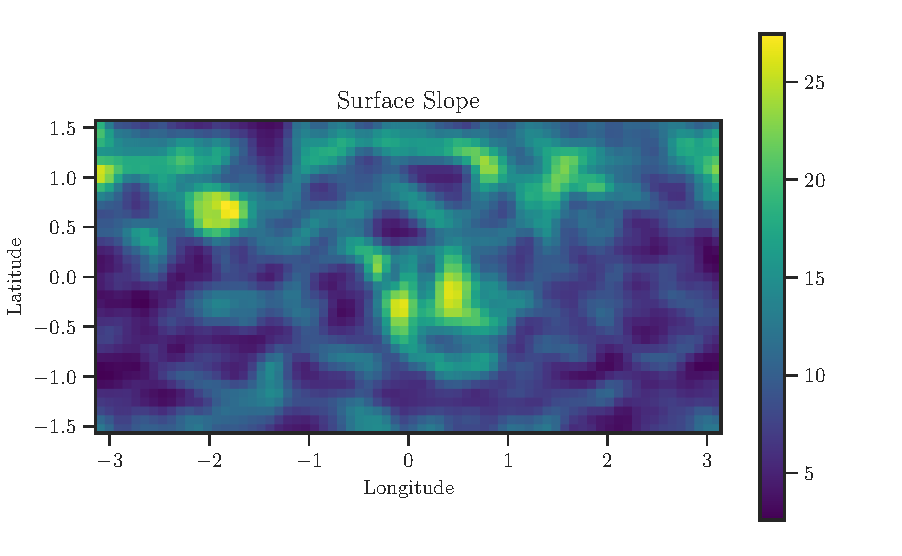
\includegraphics[width=\textwidth]{figures/computational_geometry/dynamic_exploration/castalia/refine/slope.pdf}}\\%
    \subcaptionbox{Masked surface slope with areas \( \phi > \SI{5}{\degree}\) excluded\label{fig:surface_slope_castalia_masked}}{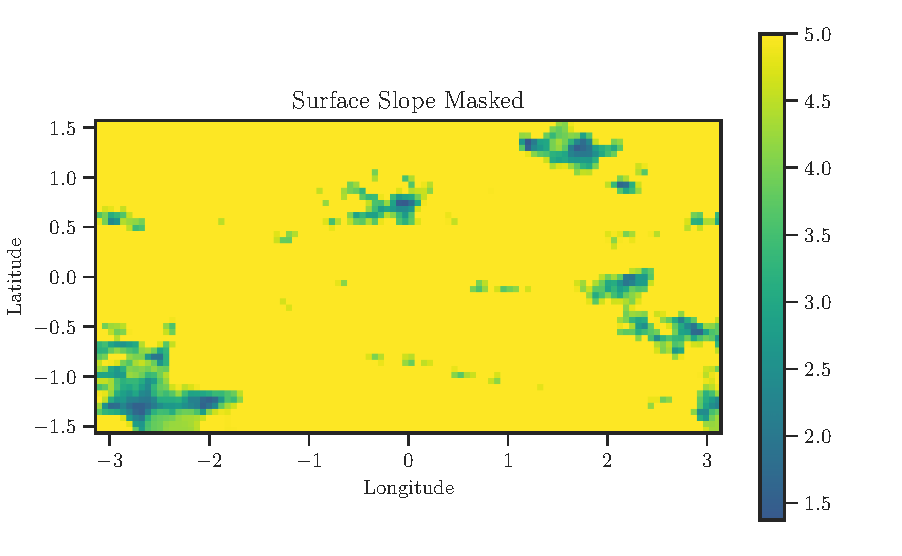
\includegraphics[width=\textwidth,keepaspectratio]{figures/computational_geometry/dynamic_exploration/castalia/refine/slope_masked.pdf}}
    \caption{Surface slope of asteroid Castalia\label{fig:surface_slope_castalia_both}}
\end{figure}

The next metric is related to the distance from the current spacecraft position to all candidate landing sites on the surface.
We utilize~\cref{eq:geodesic_distance} to compute a distance metric to the surface.
Landing sites which are closer will be considered preferentially over those at a larger distance.
\Cref{fig:distance_castalia_both} shows a surface plot of the distance to the surface. 
The area immediately beneath the spacecraft has a small cost while those on the opposite side of the asteroid have a much larger cost.
\begin{figure}[htbp]
    \centering
    \subcaptionbox{Surface Distance to surface of Castalia\label{fig:surface_distance_castalia}}{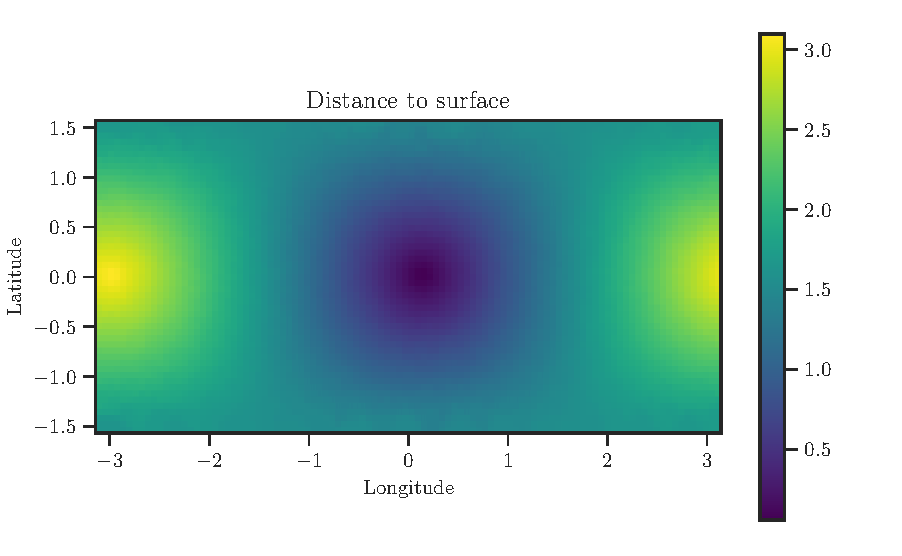
\includegraphics[width=\textwidth]{figures/computational_geometry/dynamic_exploration/castalia/refine/dist.pdf}}\\%
    \subcaptionbox{Masked distance to surface with areas \( \phi > \SI{5}{\degree}\) excluded\label{fig:surface_distance_castalia_masked}}{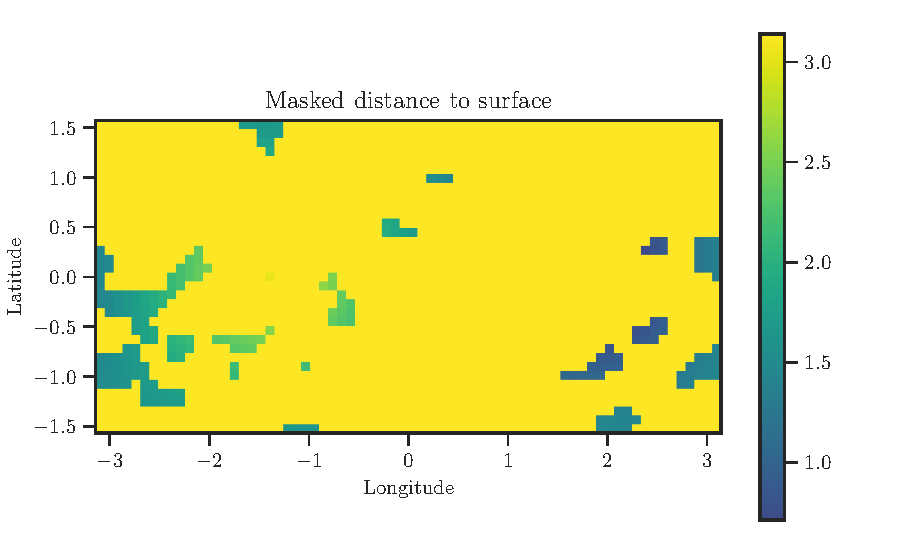
\includegraphics[width=\textwidth,keepaspectratio]{figures/computational_geometry/dynamic_exploration/castalia/refine/dist_masked.pdf}}
    \caption{Distance to surface of asteroid Castalia\label{fig:distance_castalia_both}}
\end{figure}
We can combine~\cref{fig:distance_castalia_both,fig:surface_slope_castalia_both} to determine the best landing site. 
The combination of the two is shown in~\cref{fig:landing_site_cost} with the desired landing site shown by the blue marker.
\begin{figure}[htbp]
    \centering
    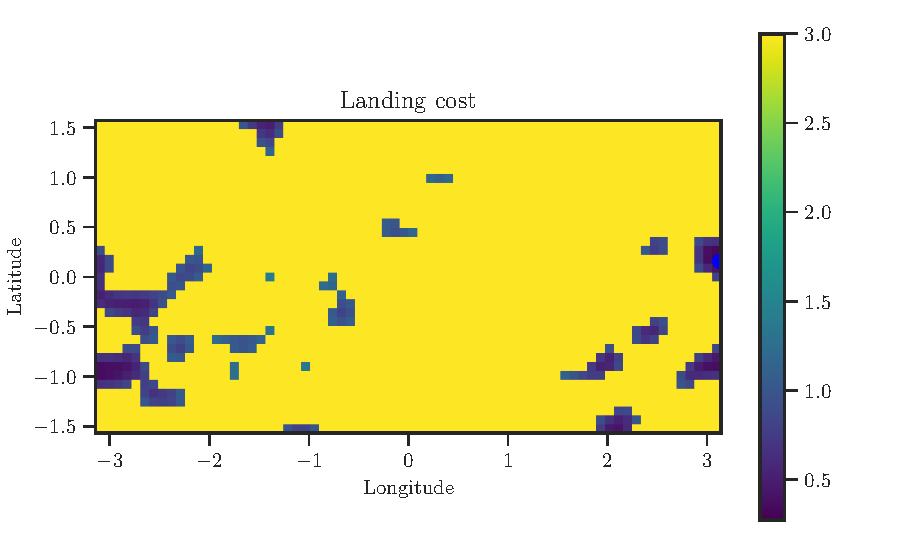
\includegraphics[width=\textwidth,keepaspectratio]{figures/computational_geometry/dynamic_exploration/castalia/refine/cost.pdf}
    \caption{Total cost for surface landing based on surface slope and distance\label{fig:landing_site_cost}}
\end{figure}
After selecting the appropriate landing site we then prepare for landing by collecting more measurements in the region around the landing area.

\paragraph{Castalia Landing Site Refinement}
One key benefit of an in-situ spacecraft is the ability to measure surface features at a much higher resolution than is possible from the ground. 
This detail provides a much higher fidelity data source than ground based measurements. 
In order to emulate this in the simulation we augment the shape model of Castalia with several small craters and outcroppings as shown in~\cref{fig:castalia_refinement}.
However, these small features would be difficult to capture with the current low resolution shape model of approximately \num{4000} faces.
The lower number of faces is useful for the evaluation of the polyhedron potential model, it is not ideal for the capture of minute surface features. 
As a result, we utilize the isotropic remeshing operation described previously to selectively increase the fidelity in the region about the desired landing site.
\Cref{fig:castalia_refine_density} shows that the vertex density increases by approximately an order of magnitude in region immediately surround the landing site.
\begin{figure}[htbp]
    \centering
    \subcaptionbox{Original vertex density of the initial shape estimate\label{fig:intial_vertex_density}}{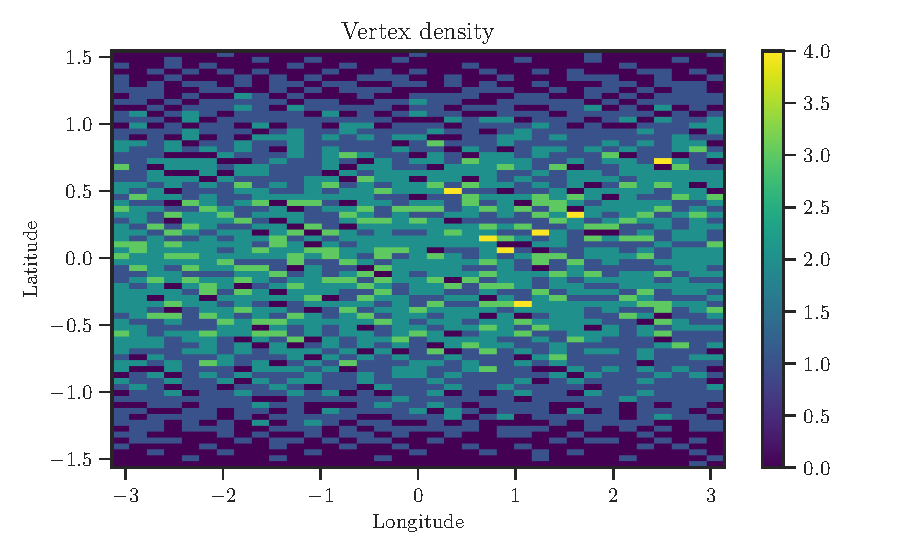
\includegraphics[width=1.0\textwidth]{figures/computational_geometry/dynamic_exploration/castalia/refine/density.pdf}}

    \subcaptionbox{Vertex density after refinement  around landing site\label{fig:refine_vertex_density}}{\includegraphics[width=1.0\textwidth]{figures/computational_geometry/dynamic_exploration/castalia/land/density.pdf}}
    \caption{Vertex density before and after refinement at asteroid Castalia\label{fig:castalia_refine_density}}
\end{figure}

The increased number of faces and vertices in the landing area allows for the capture of the small surface features.
\Cref{fig:castalia_refinement} shows that given \gls{lidar} measurements alone and the algorithm presented in~\cref{sec:radius_update} the small craters and features are effectively estimated.
\begin{figure}[htbp]
    \centering
    \subcaptionbox{Augmented shape of Castalia with surface features\label{fig:orig_castalia}}{\includegraphics[trim={15cm 0 15cm 0},clip,keepaspectratio,width=0.49\textwidth]{figures/computational_geometry/dynamic_exploration/castalia_bump_true.jpg}}~
    \subcaptionbox{Estimated shape model after measuring the surface\label{fig:bump_castalia}}{\includegraphics[trim={15cm 0 15cm 0},clip,keepaspectratio,width=0.49\textwidth]{figures/computational_geometry/dynamic_exploration/castalia_bump_est.jpg}}
    \caption{Asteroid Castalia with augmented with additional surface features~\label{fig:castalia_refinement}}
\end{figure}

\paragraph{Castalia Vertical Descent}

The final phase of the simulation is to utilize the mixed resolution model and vertically descend to the desired landing site. 
This is accomplished using the closed loop control of~\cref{sec:se3_control} and a trajectory which transitions from the home position to the surface over \SI{3600}{\second}.
The landing trajectory, using the estimated shape, is visualized in the asteroid frame in~\cref{fig:castalia_landing}.
During the vertical descent the vehicle is able to accurately track the desired trajectory using the estimated shape to compute the gravitational potential.
\begin{figure}[htbp]
    \centering
    \includegraphics[width=\textwidth]{figures/computational_geometry/dynamic_exploration/castalia/land/asteroid_trajectory.jpg}
    \caption{Vertical descent onto 4769 Castalia~\label{fig:castalia_landing}}
\end{figure}

\section{Summary}

The developments of this chapter, when combined with the details of~\cref{sec:mathematical_background,sec:lowthrust_transfers,sec:se3_control}, provide a complete approach for the operation of a spacecraft around a small body.
This chapter developed a Bayesian update scheme to reconstruct the shape of a small body from range measurements. 
The approach allows for a local update operation that is able to reconstruct the shape in real time. 
This is in contrast to standard shape reconstruction algorithms which operate over the entire surface and require signification computational resources.
Next, an optimal guidance scheme is derived which determines the desired state to best update the shape estimate. 
This allows for a spacecraft to autonomously maneuver and reconstruct the shape of a small body without operator intervention.
Finally, a mixed resolution shape representation is presented to allow for an increased fidelity in a specific region of the asteroid.
This allows for a much greater shape accuracy in a local area while avoiding the computational costs associated with a uniformly high resolution mesh.
Several numerical examples were presented which demonstrates the approach on a number of real asteroids.

\bibliographystyle{AAS_publication} 
\bibliography{library}

\end{document}
